%%%%%%%%%%%%%%%%%%%%%%% file template.tex %%%%%%%%%%%%%%%%%%%%%%%%%
%
% This is a general template file for the LaTeX package SVJour3
% for Springer journals.          Springer Heidelberg 2010/09/16
%
% Copy it to a new file with a new name and use it as the basis
% for your article. Delete % signs as needed.
%
% This template includes a few options for different layouts and
% content for various journals. Please consult a previous issue of
% your journal as needed.
%
%%%%%%%%%%%%%%%%%%%%%%%%%%%%%%%%%%%%%%%%%%%%%%%%%%%%%%%%%%%%%%%%%%%
%
% First comes an example EPS file -- just ignore it and
% proceed on the \documentclass line
% your LaTeX will extract the file if required
\begin{filecontents*}{example.eps}
%!PS-Adobe-3.0 EPSF-3.0
%%BoundingBox: 19 19 221 221
%%CreationDate: Mon Sep 29 1997
%%Creator: programmed by hand (JK)
%%EndComments
gsave
newpath
  20 20 moveto
  20 220 lineto
  220 220 lineto
  220 20 lineto
closepath
2 setlinewidth
gsave
  .4 setgray fill
grestore
stroke
grestore
\end{filecontents*}
%
\RequirePackage{fix-cm}

\documentclass{svjour3}                     % onecolumn (standard format)
%\documentclass[smallextended]{svjour3}       % onecolumn (second format)

\usepackage{hyperref}
\smartqed  % flush right qed marks, e.g. at end of proof

%\modulolinenumbers[5]

%\usepackage[utf8x]{inputenc}
\usepackage[T1]{fontenc}
\usepackage[english]{babel}
\usepackage{booktabs}
\usepackage{multirow}
\usepackage{amssymb}
\let\proof\relax
\let\endproof\relax
\usepackage{amsmath}
\renewcommand{\vec}[1]{\mathbf{#1}}
\usepackage{pst-tree}
\usepackage{graphics}
\usepackage{array}
\usepackage{changebar}
%\usepackage[math]{cellspace}

%\documentclass[vecarrow]{svmono}

\usepackage{bussproofs}
\usepackage{amsthm}
\usepackage{alltt}
\usepackage{etoolbox}
\usepackage{longtable}

%\usepackage[active,tightpage,graphics]{preview}
%\usepackage[active,tightpage,floats]{preview}
%\PreviewBorder=12pt\relax

\apptocmd{\sloppy}{\hbadness 10000\relax}{}{}

\newtheorem{defn}{Definition}[section]
\newtheorem{thm}{Theorem}[section]
%\newtheorem{lemma}{Lemma}[section]
%\newtheorem{example}{Example}[section]
%\newtheorem{proof}{Proof}
\newcommand{\crossover}[3]{\left.\sideset{_{#1}^{#3}}{_{#2}^{}}{\scriptstyle\bigotimes}\right.}
\newcommand{\Crossover}[4]{\left.\sideset{_{#1}^{#3}}{_{#2}^{#4}}\bigotimes\right.}
\newcommand{\mutation}[2]{\left.\sideset{^{#2}}{_{#1}}{\scriptstyle\bigodot}\right.}
\newcommand{\mutationtmp}[1]{\left.\sideset{}{_{#1}}{\scriptstyle\bigodot}\right.}
\newcommand{\Mutation}[3]{\left.\sideset{^{#2}}{_{#1}^{#3}}\bigodot\right.}
\newcommand{\Mutationtmp}[1]{\left.\sideset{}{_{#1}}\bigodot\right.}
%\newcommand{\Crossover}[4]{\left._{#1}\overset{#3}{\underset{#4}{\bigotimes_{#2}}}\right.}
\newcommand{\subterm}[2]{\left. #1 \right|_{#2}}
\newcommand{\replace}[3]{#1 [#2]_{#3}}
\newcommand{\normal}[2]{\left. #1 \right\downarrow_{#2}}
\newcommand{\normali}[1]{\left. #1 \right\downarrow}
\newcommand{\etaexpanded}[1]{\left. #1 \right\uparrow^{\eta}}
\newcommand{\etalong}[1]{\left. #1 \right\updownarrow^{\eta}_{\beta}}
\newcommand{\lang}[1]{\(\bf{#1}\)}
\newcommand{\pbox}[1]{\psframebox{#1}}
\newcommand{\nothing}[1]{#1}
\newcommand{\changed}[1]{#1}
\newcommand{\changeda}[1]{\cbstart#1 \cbend}



% BibTeX users please use one of
%\bibliographystyle{spbasic}      % basic style, author-year citations
\bibliographystyle{spmpsci}      % mathematics and physical sciences
%\bibliographystyle{spphys}       % APS-like style for physics
%\bibliography{}   % name your BibTeX data base


\begin{document}

%\begin{frontmatter}

\title{Higher-order Specification of Terminating Functions\\in Genetic Programming}

%\title{Higher-order specification of Genetic Programs\tnoteref{mytitlenote}}
%\tnotetext[mytitlenote]{Fully documented templates are available in the elsarticle package on \href{http://www.ctan.org/tex-archive/macros/latex/contrib/elsarticle}{CTAN}.}

%% Group authors per affiliation:
\author{Omar Monta\~no-Rivas \and C\'esar Guerra-Garc\'ia \and Moa Johansson \and Mart\'in Hern\'andez-Ordo\~nez}%\fnref{omar}}
%\author{C\'esar Guerra-Garc\'ia}%\fnref{cesar}}
%\address{Universidad Polit\'ecnica de San Luis Potos\'i,\\ Department of Information Technology,\\ Urbano Villal\'on 500, La Ladrillera,\\78369 San Luis Potos\'i, S.L.P., M\'exico.\\omar.montano@upslp.edu.mx\\cesar.guerra@upslp.edu.mx}
%\fntext[omar]{omar.montano@upslp.edu.mx}
%\fntext[cesar]{cesar.guerra@upslp.edu.mx}

%\author{Moa Johansson}%\fnref{moa}}
%\address{Chalmers University of Technology,\\ Department of Computer Science and Engineering,\\ Maskingränd 2, \\412 96 Gothenburg, Sweden.\\moa.johansson@chalmers.se}
%\fntext[moa]{moa.johansson@chalmers.se}

%\author{Mart\'in Hern\'andez-Ordo\~nez}%\fnref{martin}}
%\address{Universidad Polit\'ecnica de Victoria,\\Department of Mechatronics,\\Carretera Victoria-Soto la Marina Km. 5.5,\\Parque Cient\'ifico y Tecnol\'ogico de Tamaulipas,\\ 87138 Ciudad Victoria, Tam. M\'exico.\\mhernandezo@upv.edu.mx}

\institute{Omar Monta\~no-Rivas and C\'esar Guerra-Garc\'ia \at
              Universidad Polit\'ecnica de San Luis Potos\'i, Department of Information Technology,\\ Urbano Villal\'on 500, La Ladrillera,78369 San Luis Potos\'i, S.L.P., M\'exico.\\\email{omar.montano@upslp.edu.mx}\\\email{cesar.guerra@upslp.edu.mx}
           \and
           Moa Johansson \at
              Chalmers University of Technology, Department of Computer Science and Engineering,\\ Maskingr\"and 2, 412 96 Gothenburg, Sweden.\\\email{moa.johansson@chalmers.se} \and
           Mart\'in Hern\'andez-Ordo\~nez \at
              Universidad Polit\'ecnica de Victoria, Department of Mechatronics,\\Carretera Victoria-Soto la Marina Km. 5.5,Parque Cient\'ifico y Tecnol\'ogico de Tamaulipas, 87138 Ciudad Victoria, Tam. M\'exico.\\\email{mhernandezo@upv.edu.mx}
}

\date{Received: date / Accepted: date}
% The correct dates will be entered by the editor

\maketitle

%\fntext[martin]{mhernandezo@upv.edu.mx}

%\fntext[upslp]{Universidad Polit\'ecnica de San Luis Potos\'i, Urbano Villal\'on 500, La Ladrillera, 78369 San Luis Potos\'i, S.L.P., M\'exico.}


\begin{abstract}
%A fundamental problem in genetic programming is the description of the solution space to restrict the search. This paper present a logical specification of the solution space using higher order formulas and describe the application of evolving total computable functions in inductive theories. We report the computational effort required to evolve addition and multiplication of natural numbers, odd, even and the Ackermann functions. We found that the specification mechanism based in higher-order formulas is flexible enough to represent different kinds of recursion, even general recursion. The techniques described are implemented in the proof assistant Isabelle.
  A fundamental problem in genetic programming is the description of the solution space to restrict the search.

  This paper present a logical specification of a Genetic Programming problem using higher order formulas. Our representation has three notorious advantages: it provides a framework to describe the solution space, this framework can be used to restrict the search space

  Our technique allows to prove well-definedness properties, such as termination, of synthesized functions using standard facilities in proof assistants. We describe the application of evolving total computable functions in inductive theories. We report the computational effort required to evolve summation over lists, addition and multiplication of natural numbers, odd, even and the Ackermann function. We found that the specification mechanism based in higher-order formulas is flexible enough to represent different kinds of recursion, even general recursion. The techniques described are implemented in the interactive proof assistant Isabelle.
  \keywords{genetic programming\and lambda calculus\and recursion\and term-rewriting\and termination\and proof assistant}
\end{abstract}

%\begin{keyword}
%genetic programming\sep lambda calculus\sep recursion\sep term-rewriting\sep termination\sep proof assistant
%\MSC[2010] 03B15\sep  03D20\sep 68N18\sep 16S15
%\end{keywords}

%\end{frontmatter}

%\linenumbers

\section{Introduction}
\label{introduction}
Genetic programming (GP) is a machine learning technique used to generate a computer program to solve a specified problem. It uses a stochastic algorithm inspired by biological evolution to search through a space of possible programs for one that performs ``well'' according to a fitness function.

A fundamental problem in genetic programming is the description of the solution space to restrict the search. This description needs to be general and flexible enough to represent different kinds of recursion such as primitive recursion, mutual recursion, or even general recursion.

One simple example, to illustate our approach, would be to evolve a program to sum the elements of a list. Here a preliminary step in a canonical GP run is to define the terminal and function set. The set usually found in literature for this problem is the if-then-else construct $IF$ ($\lambda x\,y\,z.\ if\ x\ then\ y\ else\ z$), equality over lists ($=$) and the empty list ($[]$), addition of natural numbers ($+$) and its neutral element ($0$), the destructor functions $head$ and $tail$ which separates a lists into its constituent elements, and finally the same function to be defined in order to perform recursion (e.g. $f$). As stated in (\ref{intro-destructive-style-sum-scheme}), the problem now is to find a function $f$ defined in terms of the terminal and function set such that some property $P$ holds\footnote{$P$ is defined in terms of some fitness function.}.

\begin{equation}
  \exists f.\,\, (\forall xs.\ f\ xs\ = N\ xs\ IF\ (=)\ []\ (+)\ 0\ hd\ tl\ f)
  \land (P\ f)
  \label{intro-destructive-style-sum-scheme}
\end{equation}

%The search space for this problem is made explicit with the help of the {\em meta-variable} $N$.

Intuitively, $N$ is a function which provides the computational content to $f$ and here is used as a medium to explicitly describe the search space for this problem. In this work, we view the search space for this problem as the set\footnote{Or more precisely, the set of substitutions of the form $\{N \mapsto t\}$ where $t$ is a typed pure $\lambda$-lambda term.} of (typed) pure $\lambda$-terms $N$ such that equation (\ref{destructor-style-eq}) holds.
\begin{equation}
  \label{destructor-style-eq}
  f\ xs = N\ xs\ IF\ (=)\ []\ (+)\ 0\ head\ tail\ f.
\end{equation}
%The number of terms in this set will depend on the size of the term (see \ref{notations}).
This view of the search space has one big advantage. The problem to describe the search space of a GP problem is translated into the well known and understood problem to count and generate $\lambda$-terms. For example, we may have an idea of how difficult is a GP problem by counting the number of $\lambda$-terms up to a given size~\cite{hindley1997basic,zaionc1995fixpoint,wang2005generating}. Or we can use ~\cite{hindley1997basic,takahashi1996normal,wang2005generating}

Depending on the value of $N$, the induced definition will be well-defined or not. For example, the $\lambda$-term $(\lambda a\, b\, c\, \-d\,\- e\,\- f\, g\, h\, i.\ a)$ induces a well-defined function as it yields the identity function $f\ xs = xs$ as opposed to the $\lambda$-term $(\lambda a\, b\, c\, \-d\,\- e\,\- f\, g\, h\, i.\ i\ a)$ as it yields the non-terminating function $f\ xs = f\ xs$. A $\lambda$-term that synthesizes the target function for this problem could be $(\lambda a\, b\, c\, \-d\,\- e\,\- f\, g\, h\, i.\ b\ (c\ d\ a)\ f\ (e\ (g\ a)\ (i\ (h\ a))))$ as it yields, after $\beta$-contraction, the following definition.
$$
f\ xs = (if\ [] = xs\ then\ 0\ else\ hd\ xs\ +\ f\ (tl\ xs)).
$$

In (typed) functional programming languages such as Haskell or SML, it is more common to define recursive functions by pattern matching if the function is being defined recursively on an inductive datatype. For our simple example, Equation \ref{destructor-style-eq} can be phrased using pattern matching as
\begin{equation}
  \label{contructor-style-eq}
  \begin{array}{rcl}
    f\ [] & = & 0\\
    f\ (x \# xs) & = & M\ x\ xs\ (+)\ f.
  \end{array}
\end{equation}

Note that we do not need equality on lists or the construct if-then-else because the distinction between empty and non-empty lists is made explicit using the two patterns of definition (\ref{contructor-style-eq}). The destructors $head$ and $tail$ are also not needed because the constructor $Cons$ ($\#$) is used in the left hand side of the second equation of (\ref{contructor-style-eq}) to separate the head from the tail of the list. Here again, $M$ is a set of $\lambda$-terms with adequate type that describe the new search space, but contrary to the previous example, the new search space contains only well-defined functions, i.e. it defines primitive recursive functions. The target function can be synthesized with the $\lambda$-term $(\lambda a\, b\, c\, d.\ c\ a\ (d\ b))$ for $M$. This yields the following definition.
$$
\begin{array}{rcl}
  f\ [] & = &0\\
  f\ (x \# xs) & = & x + f\ xs.
\end{array}
$$

Constructor style definitions are usually preferred over destructor style in functional languages because they are more natural and resilient to the problem of partiality of destructive functions, e.g. applying $head$ to an empty list would lead to an exception. Constructor style definitions are also normally shorter, which would imply searching for smaller terms in the search space. Figure \ref{destructive_vs_constructive} shows the number of $\lambda$-terms in the search space as a function of the term size for the destructor and constructor styles of definitions (\ref{destructor-style-eq}) and (\ref{contructor-style-eq}) respectively.
\begin{figure}[!ht]
  \centering
    \scalebox{0.6}{
      % GNUPLOT: LaTeX picture
\setlength{\unitlength}{0.240900pt}
\ifx\plotpoint\undefined\newsavebox{\plotpoint}\fi
\sbox{\plotpoint}{\rule[-0.200pt]{0.400pt}{0.400pt}}%
\begin{picture}(1500,900)(0,0)
\sbox{\plotpoint}{\rule[-0.200pt]{0.400pt}{0.400pt}}%
\put(211.0,131.0){\rule[-0.200pt]{4.818pt}{0.400pt}}
\put(191,131){\makebox(0,0)[r]{$1$}}
\put(1419.0,131.0){\rule[-0.200pt]{4.818pt}{0.400pt}}
\put(211.0,196.0){\rule[-0.200pt]{4.818pt}{0.400pt}}
\put(191,196){\makebox(0,0)[r]{$10$}}
\put(1419.0,196.0){\rule[-0.200pt]{4.818pt}{0.400pt}}
\put(211.0,260.0){\rule[-0.200pt]{4.818pt}{0.400pt}}
\put(191,260){\makebox(0,0)[r]{$100$}}
\put(1419.0,260.0){\rule[-0.200pt]{4.818pt}{0.400pt}}
\put(211.0,325.0){\rule[-0.200pt]{4.818pt}{0.400pt}}
\put(191,325){\makebox(0,0)[r]{$1000$}}
\put(1419.0,325.0){\rule[-0.200pt]{4.818pt}{0.400pt}}
\put(211.0,389.0){\rule[-0.200pt]{4.818pt}{0.400pt}}
\put(191,389){\makebox(0,0)[r]{$10000$}}
\put(1419.0,389.0){\rule[-0.200pt]{4.818pt}{0.400pt}}
\put(211.0,454.0){\rule[-0.200pt]{4.818pt}{0.400pt}}
\put(191,454){\makebox(0,0)[r]{$100000$}}
\put(1419.0,454.0){\rule[-0.200pt]{4.818pt}{0.400pt}}
\put(211.0,518.0){\rule[-0.200pt]{4.818pt}{0.400pt}}
\put(191,518){\makebox(0,0)[r]{$1e+06$}}
\put(1419.0,518.0){\rule[-0.200pt]{4.818pt}{0.400pt}}
\put(211.0,583.0){\rule[-0.200pt]{4.818pt}{0.400pt}}
\put(191,583){\makebox(0,0)[r]{$1e+07$}}
\put(1419.0,583.0){\rule[-0.200pt]{4.818pt}{0.400pt}}
\put(211.0,647.0){\rule[-0.200pt]{4.818pt}{0.400pt}}
\put(191,647){\makebox(0,0)[r]{$1e+08$}}
\put(1419.0,647.0){\rule[-0.200pt]{4.818pt}{0.400pt}}
\put(211.0,712.0){\rule[-0.200pt]{4.818pt}{0.400pt}}
\put(191,712){\makebox(0,0)[r]{$1e+09$}}
\put(1419.0,712.0){\rule[-0.200pt]{4.818pt}{0.400pt}}
\put(211.0,776.0){\rule[-0.200pt]{4.818pt}{0.400pt}}
\put(191,776){\makebox(0,0)[r]{$1e+10$}}
\put(1419.0,776.0){\rule[-0.200pt]{4.818pt}{0.400pt}}
\put(211.0,131.0){\rule[-0.200pt]{0.400pt}{4.818pt}}
\put(211,90){\makebox(0,0){$5$}}
\put(211.0,756.0){\rule[-0.200pt]{0.400pt}{4.818pt}}
\put(347.0,131.0){\rule[-0.200pt]{0.400pt}{4.818pt}}
\put(347,90){\makebox(0,0){$10$}}
\put(347.0,756.0){\rule[-0.200pt]{0.400pt}{4.818pt}}
\put(484.0,131.0){\rule[-0.200pt]{0.400pt}{4.818pt}}
\put(484,90){\makebox(0,0){$15$}}
\put(484.0,756.0){\rule[-0.200pt]{0.400pt}{4.818pt}}
\put(620.0,131.0){\rule[-0.200pt]{0.400pt}{4.818pt}}
\put(620,90){\makebox(0,0){$20$}}
\put(620.0,756.0){\rule[-0.200pt]{0.400pt}{4.818pt}}
\put(757.0,131.0){\rule[-0.200pt]{0.400pt}{4.818pt}}
\put(757,90){\makebox(0,0){$25$}}
\put(757.0,756.0){\rule[-0.200pt]{0.400pt}{4.818pt}}
\put(893.0,131.0){\rule[-0.200pt]{0.400pt}{4.818pt}}
\put(893,90){\makebox(0,0){$30$}}
\put(893.0,756.0){\rule[-0.200pt]{0.400pt}{4.818pt}}
\put(1030.0,131.0){\rule[-0.200pt]{0.400pt}{4.818pt}}
\put(1030,90){\makebox(0,0){$35$}}
\put(1030.0,756.0){\rule[-0.200pt]{0.400pt}{4.818pt}}
\put(1166.0,131.0){\rule[-0.200pt]{0.400pt}{4.818pt}}
\put(1166,90){\makebox(0,0){$40$}}
\put(1166.0,756.0){\rule[-0.200pt]{0.400pt}{4.818pt}}
\put(1303.0,131.0){\rule[-0.200pt]{0.400pt}{4.818pt}}
\put(1303,90){\makebox(0,0){$45$}}
\put(1303.0,756.0){\rule[-0.200pt]{0.400pt}{4.818pt}}
\put(1439.0,131.0){\rule[-0.200pt]{0.400pt}{4.818pt}}
\put(1439,90){\makebox(0,0){$50$}}
\put(1439.0,756.0){\rule[-0.200pt]{0.400pt}{4.818pt}}
\put(211.0,131.0){\rule[-0.200pt]{0.400pt}{155.380pt}}
\put(211.0,131.0){\rule[-0.200pt]{295.825pt}{0.400pt}}
\put(1439.0,131.0){\rule[-0.200pt]{0.400pt}{155.380pt}}
\put(211.0,776.0){\rule[-0.200pt]{295.825pt}{0.400pt}}
\put(30,453){\makebox(0,0){\rotatebox{90}{$\lambda$-terms}}}
\put(825,29){\makebox(0,0){size}}
\put(825,838){\makebox(0,0){Number of typed lambda terms}}
\put(1279,735){\makebox(0,0)[r]{Destructive style}}
\put(1299.0,735.0){\rule[-0.200pt]{24.090pt}{0.400pt}}
\put(347,131){\usebox{\plotpoint}}
\multiput(347.00,131.58)(0.611,0.498){87}{\rule{0.589pt}{0.120pt}}
\multiput(347.00,130.17)(53.778,45.000){2}{\rule{0.294pt}{0.400pt}}
\multiput(402.00,176.58)(1.389,0.496){37}{\rule{1.200pt}{0.119pt}}
\multiput(402.00,175.17)(52.509,20.000){2}{\rule{0.600pt}{0.400pt}}
\multiput(457.00,196.58)(1.238,0.496){41}{\rule{1.082pt}{0.120pt}}
\multiput(457.00,195.17)(51.755,22.000){2}{\rule{0.541pt}{0.400pt}}
\multiput(511.00,218.58)(1.154,0.496){45}{\rule{1.017pt}{0.120pt}}
\multiput(511.00,217.17)(52.890,24.000){2}{\rule{0.508pt}{0.400pt}}
\multiput(566.00,242.58)(1.133,0.496){45}{\rule{1.000pt}{0.120pt}}
\multiput(566.00,241.17)(51.924,24.000){2}{\rule{0.500pt}{0.400pt}}
\multiput(620.00,266.58)(0.953,0.497){55}{\rule{0.859pt}{0.120pt}}
\multiput(620.00,265.17)(53.218,29.000){2}{\rule{0.429pt}{0.400pt}}
\multiput(675.00,295.58)(0.874,0.497){59}{\rule{0.797pt}{0.120pt}}
\multiput(675.00,294.17)(52.346,31.000){2}{\rule{0.398pt}{0.400pt}}
\multiput(729.00,326.58)(0.920,0.497){57}{\rule{0.833pt}{0.120pt}}
\multiput(729.00,325.17)(53.270,30.000){2}{\rule{0.417pt}{0.400pt}}
\multiput(784.00,356.58)(0.890,0.497){59}{\rule{0.810pt}{0.120pt}}
\multiput(784.00,355.17)(53.319,31.000){2}{\rule{0.405pt}{0.400pt}}
\multiput(839.00,387.58)(0.846,0.497){61}{\rule{0.775pt}{0.120pt}}
\multiput(839.00,386.17)(52.391,32.000){2}{\rule{0.388pt}{0.400pt}}
\multiput(893.00,419.58)(0.890,0.497){59}{\rule{0.810pt}{0.120pt}}
\multiput(893.00,418.17)(53.319,31.000){2}{\rule{0.405pt}{0.400pt}}
\multiput(948.00,450.58)(0.846,0.497){61}{\rule{0.775pt}{0.120pt}}
\multiput(948.00,449.17)(52.391,32.000){2}{\rule{0.388pt}{0.400pt}}
\multiput(1002.00,482.58)(0.862,0.497){61}{\rule{0.788pt}{0.120pt}}
\multiput(1002.00,481.17)(53.366,32.000){2}{\rule{0.394pt}{0.400pt}}
\multiput(1057.00,514.58)(0.862,0.497){61}{\rule{0.788pt}{0.120pt}}
\multiput(1057.00,513.17)(53.366,32.000){2}{\rule{0.394pt}{0.400pt}}
\multiput(1112.00,546.58)(0.846,0.497){61}{\rule{0.775pt}{0.120pt}}
\multiput(1112.00,545.17)(52.391,32.000){2}{\rule{0.388pt}{0.400pt}}
\multiput(1166.00,578.58)(0.836,0.497){63}{\rule{0.767pt}{0.120pt}}
\multiput(1166.00,577.17)(53.409,33.000){2}{\rule{0.383pt}{0.400pt}}
\multiput(1221.00,611.58)(0.820,0.497){63}{\rule{0.755pt}{0.120pt}}
\multiput(1221.00,610.17)(52.434,33.000){2}{\rule{0.377pt}{0.400pt}}
\multiput(1275.00,644.58)(0.836,0.497){63}{\rule{0.767pt}{0.120pt}}
\multiput(1275.00,643.17)(53.409,33.000){2}{\rule{0.383pt}{0.400pt}}
\multiput(1330.00,677.58)(0.820,0.497){63}{\rule{0.755pt}{0.120pt}}
\multiput(1330.00,676.17)(52.434,33.000){2}{\rule{0.377pt}{0.400pt}}
\multiput(1384.00,710.58)(0.836,0.497){63}{\rule{0.767pt}{0.120pt}}
\multiput(1384.00,709.17)(53.409,33.000){2}{\rule{0.383pt}{0.400pt}}
\put(347,131){\makebox(0,0){$+$}}
\put(402,176){\makebox(0,0){$+$}}
\put(457,196){\makebox(0,0){$+$}}
\put(511,218){\makebox(0,0){$+$}}
\put(566,242){\makebox(0,0){$+$}}
\put(620,266){\makebox(0,0){$+$}}
\put(675,295){\makebox(0,0){$+$}}
\put(729,326){\makebox(0,0){$+$}}
\put(784,356){\makebox(0,0){$+$}}
\put(839,387){\makebox(0,0){$+$}}
\put(893,419){\makebox(0,0){$+$}}
\put(948,450){\makebox(0,0){$+$}}
\put(1002,482){\makebox(0,0){$+$}}
\put(1057,514){\makebox(0,0){$+$}}
\put(1112,546){\makebox(0,0){$+$}}
\put(1166,578){\makebox(0,0){$+$}}
\put(1221,611){\makebox(0,0){$+$}}
\put(1275,644){\makebox(0,0){$+$}}
\put(1330,677){\makebox(0,0){$+$}}
\put(1384,710){\makebox(0,0){$+$}}
\put(1439,743){\makebox(0,0){$+$}}
\put(1349,735){\makebox(0,0){$+$}}
\put(1279,694){\makebox(0,0)[r]{Constructive style}}
\multiput(1299,694)(20.756,0.000){5}{\usebox{\plotpoint}}
\put(1399,694){\usebox{\plotpoint}}
\put(211,131){\usebox{\plotpoint}}
\multiput(211,131)(19.618,6.777){3}{\usebox{\plotpoint}}
\multiput(266,150)(20.261,4.503){3}{\usebox{\plotpoint}}
\multiput(320,162)(20.114,5.120){3}{\usebox{\plotpoint}}
\multiput(375,176)(20.179,4.858){2}{\usebox{\plotpoint}}
\multiput(429,189)(19.929,5.798){3}{\usebox{\plotpoint}}
\multiput(484,205)(19.900,5.896){3}{\usebox{\plotpoint}}
\multiput(538,221)(19.726,6.456){3}{\usebox{\plotpoint}}
\multiput(593,239)(19.726,6.456){2}{\usebox{\plotpoint}}
\multiput(648,257)(19.463,7.209){3}{\usebox{\plotpoint}}
\multiput(702,277)(19.618,6.777){3}{\usebox{\plotpoint}}
\multiput(757,296)(19.344,7.523){3}{\usebox{\plotpoint}}
\multiput(811,317)(19.390,7.404){3}{\usebox{\plotpoint}}
\multiput(866,338)(19.390,7.404){2}{\usebox{\plotpoint}}
\multiput(921,359)(19.344,7.523){3}{\usebox{\plotpoint}}
\multiput(975,380)(19.390,7.404){3}{\usebox{\plotpoint}}
\multiput(1030,401)(19.222,7.831){3}{\usebox{\plotpoint}}
\multiput(1084,423)(19.271,7.708){3}{\usebox{\plotpoint}}
\multiput(1139,445)(19.222,7.831){3}{\usebox{\plotpoint}}
\multiput(1193,467)(19.271,7.708){2}{\usebox{\plotpoint}}
\multiput(1248,489)(19.271,7.708){3}{\usebox{\plotpoint}}
\multiput(1303,511)(19.222,7.831){3}{\usebox{\plotpoint}}
\multiput(1357,533)(19.149,8.008){3}{\usebox{\plotpoint}}
\put(1412,556){\usebox{\plotpoint}}
\put(211,131){\makebox(0,0){$\times$}}
\put(266,150){\makebox(0,0){$\times$}}
\put(320,162){\makebox(0,0){$\times$}}
\put(375,176){\makebox(0,0){$\times$}}
\put(429,189){\makebox(0,0){$\times$}}
\put(484,205){\makebox(0,0){$\times$}}
\put(538,221){\makebox(0,0){$\times$}}
\put(593,239){\makebox(0,0){$\times$}}
\put(648,257){\makebox(0,0){$\times$}}
\put(702,277){\makebox(0,0){$\times$}}
\put(757,296){\makebox(0,0){$\times$}}
\put(811,317){\makebox(0,0){$\times$}}
\put(866,338){\makebox(0,0){$\times$}}
\put(921,359){\makebox(0,0){$\times$}}
\put(975,380){\makebox(0,0){$\times$}}
\put(1030,401){\makebox(0,0){$\times$}}
\put(1084,423){\makebox(0,0){$\times$}}
\put(1139,445){\makebox(0,0){$\times$}}
\put(1193,467){\makebox(0,0){$\times$}}
\put(1248,489){\makebox(0,0){$\times$}}
\put(1303,511){\makebox(0,0){$\times$}}
\put(1357,533){\makebox(0,0){$\times$}}
\put(1412,556){\makebox(0,0){$\times$}}
\put(1349,694){\makebox(0,0){$\times$}}
\put(211.0,131.0){\rule[-0.200pt]{0.400pt}{155.380pt}}
\put(211.0,131.0){\rule[-0.200pt]{295.825pt}{0.400pt}}
\put(1439.0,131.0){\rule[-0.200pt]{0.400pt}{155.380pt}}
\put(211.0,776.0){\rule[-0.200pt]{295.825pt}{0.400pt}}
\end{picture}
}
  \caption{Logarithmic graph showing the number of $\lambda$-terms using the destructor style definition (\ref{destructor-style-eq}) vs the constructor style definition (\ref{contructor-style-eq}).}
  \label{destructive_vs_constructive}
\end{figure}

Mutual recursion is a form of defining functions via recursion involving several functions simultaneously. A standard example of mutual recursion is determining whether a natural number is even or odd by having two separate functions that call each other. A constructor style setting for a GP describing this problem is to consider the following definition (\ref{contructor-style-eq-mutual-rec}), where $0$ is zero, $s$ is the successor constructor for natural numbers and $f$ and $g$ are the mutually recursive functions to be defined
\begin{equation}
  \label{contructor-style-eq-mutual-rec}
  \begin{array}{rcl}
    f\ 0 & = & true\\
    f\ (s\ n) & = & M\ 0\ s\ n\ g\\
    g\ 0 & = & false\\
    g\ (s\ n) & = & N\ 0\ s\ n\ f.
  \end{array}
\end{equation}

A solution for the target functions is obtained with the following substitution $\{M \mapsto (\lambda a\,b\,c\,d.\ d\ c), N \mapsto (\lambda a\,b\,c\,d.\ d\ c)\}$.

\cbstart
In this work we propose to use higher-order formulas to represent (and restrict) the set of functions we intend to explore during search. {\em Point-Typing} mutation and crossover (see \cite{koza1994genetic}) can be easily adapted to work with our representation of individuals as {\em substitutions} (see Section \ref{subsec:crossover-mutation} for a formal description). For example, a {\em curried} version for {\em point-typing} mutation is depicted with the individual $\{N \mapsto (\lambda a\, b\, c\, \-d\,\- e\,\- f\, g\, h\, i.\ b\ (c\ d\ a)\ f\ (e\ (g\ a)\ (i\ a)))\}$ from equation (\ref{destructor-style-eq}). The individual is non-terminating as it yields, after $\beta$-contraction, the definition
$$
f\ xs = (if\ [] = xs\ then\ 0\ else\ hd\ xs\ +\ f\ xs).
$$

Mutation can be performed on the individual by exchanging subterm $(i\ a)$ (after $\beta$-contraction $f\ xs$) by $(i\ (h\ a))$ (after $\beta$-contraction $f\ (tl\ xs)$) synthesizing the target function. An example for a {\em two-parents} crossover is depicted with the previous individual and $\{N \mapsto (\lambda a\, b\, c\, \-d\,\- e\,\- f\, g\, h\, i.\ b\ (c\ d\ a)\ f\-\ (e\-\ (g\ (h\ a))\-\ (i\ (h\ a))))\}$ (definition $f\ xs = (if\ [] = xs\ then\ 0\ else\ (head\ (tl\ xs))\ +\ f\ (tl\ xs))$) by exchanging the subterm $(i\ a)$ of first individual with $(i\ (h\ a))$ of second individual yielding the target function.
\cbend

An advantage of using our schematic representation of the problem is that we can use syntactic methods to determine whether two individuals (programs) are equivalent to avoid unnecessary recalculations (see \ref{subsec:equivalence}).

This paper present a formal description of a logical specification of the solution space of functions in a genetic programming algorithm using higher order formulas. This specification allows to synthesize higher-order functions using different recursion schemes (Section \ref{sec:synthesis}). \cbstart Individuals are represented by {\it substitutions} and classical GP operators, such as mutation and crossover, are easily defined\cbend. Well-definedness properties of synthesized functions can be proved by standard facilities, e.g. those provided by an interactive proof assistant such as Isabelle/HOL (Section \ref{subsec:termination}). A syntactic method to detect equivalent functions based on {\it normalization} is then described in Section \ref{subsec:equivalence}. Section \ref{subsec:gp-algorithm} describes the overall genetic programming algorithm and the results and discussions over the conducted case studies are reported in Section \ref{sec:results}. Previous related work and preliminary concepts and notations are presented in Section \ref{materials-methods}.

\cbstart
Although synthesis of algorithms has been studied by different research fields such as inductive programming and deductive program synthesis. In this work we concentrate on genetic programming problems assuming there is a fitness function that is to be minimized/maximized.
\cbend

%An overall genetic programming algorithm is described in 

%Section \ref{sec:synthesis} describes a formalization to synthesize higher-order functions. Aspects of well-definedness properties are covered in section \ref{subsec:termination}. The crossover and mutation operators are defined in section \ref{subsec:crossover-mutation}. A syntactic method to detect equivalent functions based on normalization is described in \ref{subsec:equivalence}. Section \ref{subsec:gp-algorithm} described the overall genetic programming algorithm. The results and discussions over the conducted case studies are reported in section \ref{sec:results}.

%This paper present a formal description of a logical specification of the solution space using higher order formulas and describe the application of evolving total computable functions in inductive theories. We report the computational effort required to evolve different inductive functions in both, destructive and constructive-style GP settings.

\section{Background}
\label{materials-methods}

\subsection{Related Work}
\label{related-work}
\cbstart
Other than this work, the {\it PolyGP system}~\cite{yu1998polygp} and the System F-based GP system \cite{binard2008genetic} are both based on the lambda calculus. The type system ensures that all programs created are type-correct. PolyGP uses a Curry style representation of terms and uses a type unification algorithm to infer types. It is implemented in Haskell and uses different kind of type variables to obtain polymorphism. Redundant expressions in parse trees (introns) are never re-evaluated as Haskell is a non-strict language (uses lazy evaluation). The purity of Haskell, however, has important computational complexity implications during the execution of the system. The crossover operator in the {\it PolyGP system} first selects a position from the first parent and then the type of the subterm at that position is used to select a crossover point in the second parent. This selection scheme is biased to prefer crossover points at positions closer to the root of the term. For the mutation operator, a position is first selected using the described selection scheme. A new term is constructed with the same type of the subterm at the selected position. Finally the new term replaces the subtree at the selected node. Mutation and crossover can be performed on partial or full application nodes but are restricted to produce terms with a maximum depth.

The System F-based GP system \cite{binard2008genetic} uses a second order (polymorphic) type system (System F). Since type checking is not decidable in the type system (see \cite{wells1999typability}), the authors used a Church style representation, where terms were annotated with enough type information. In the GP system, parse trees contain types and types are evolved at the same level as programs (terms). Since System F is strongly normalizable, only total recursive functions are expressible and thus, the primitive recursive functions are contained as a proper subclass.

Probably \cite{kahrs2006genetic} is the most relevant related work. In the aforementioned work, the author used two control operators to restrict the search space. The composition operator $Cn[f, g_1, \ldots, g_n]$ was defined as the following function application in uncurried form $f(g_1(\overline{x}), \ldots, g_n(\overline{x}))$ and the primitive recursion operator $Pr[f,g]$ was used to define the following primitive recursive functions:

\begin{equation}
  \begin{array}{rcl}
    h(0,\overline{x}) & = & f(\overline{x})\\
    h(n+1,\overline{x}) & = & g(h(n,\overline{x}),n,\overline{x}).
  \end{array}
\end{equation}

While the $Pr$ operator is reminiscent to our definition of functional scheme, it has several differences summarized in table \ref{tab:related1}.

\begin{table}[ht!]
  \centering
  \begin{tabular}{llp{4cm}}
    \toprule
    Description & $Pr$ operator & Functional schemes\\
    \toprule
    Application & Curried & Uncurried\\
    Foundation & first-order & higher-order (HOL)\\
    $\lambda$-terms & no & yes\\
    Mutual recursion & no & yes\\
    Total recursion & no & yes\\
    Pattern matching & naturals & inductive datatype\\
    User-modifiable scheme & no & yes\\
    Induce terminating functions & yes & yes using its terminating closure\\
    Superpolynomial functions & yes & yes\\
    \bottomrule
  \end{tabular}
  \caption{Differences between the $Pr$ operator and functional schemes.}
  \label{tab:related1}
\end{table}

\cbend

\subsection{Terms of Typed Lambda Calculus}
\label{sec:terms-typed-lambda-calculus}
We mainly follow the notation in \cite{Mayr-Nipkow-TCS}. Given a finite set $\mathcal{S}$ of {\em type symbols}, and a denumerable set $\mathcal{S^{\forall}}$ of {\em type variables}, the set $\mathcal{T_{\mathcal{S^{\forall}}}}$ of {\em polymorphic types} is generated from these sets by the constructor $\to$ for {\em functional types}. 
%In the following we use  $\tau$ and $\rho$ to denote types and $`a$, $`b$, etc. to denote type variables. 
The type constructor $\to$ associates to the right: read $\tau_1 \to \tau_2 \to \tau_3$ as $\tau_1 \to (\tau_2 \to \tau_3)$. \changeda{Let $\tau$ be a type $\tau_1\to \ldots \to \tau_n \to \tau_0$ where $\tau_0 \in \mathcal{S}$ and $n\geq 0$. We will sometimes write $\overline{\tau_n}\to \tau_0$ for $\tau$.}
%The arity of the type $\tau$ is $n$ and its argument types are $\tau_1,\ldots, \tau_n$. 
A {\em signature} is a set of typed {\em function symbols} denoted by $\mathcal{F} = \bigcup_{\tau \in \mathcal{T_{\mathcal{S^{\forall}}}}} \mathcal{F}_{\tau}$. Terms are generated from a set of typed {\em variables} $\mathcal{V} = \bigcup_{\tau \in \mathcal{T_{\mathcal{S^{\forall}}}}} \mathcal{V}_{\tau}$ and a signature $\mathcal{F}$ 
%where $\mathcal{F} \cap \mathcal{V} = \emptyset$ 
by $\lambda$-abstraction and application and are denoted by $\mathcal{T}(\mathcal{F},\mathcal{V})$. We write $t:\tau$ to indicate that the term $t$ has type $\tau$.

Typing rules restrict the set of terms $\mathcal{T}(\mathcal{F},\mathcal{V})$ as follows:
\begin{displaymath}
\begin{array}{cccc}
\AxiomC{$x \in \mathcal{V}_{\tau}$}
\UnaryInfC{$x : \tau$}
\DisplayProof \,\,\,\,\,\,\,\,\,&
\AxiomC{$f \in \mathcal{F}_{\tau}$}
\UnaryInfC{$f : \tau$}
\DisplayProof \,\,\,\,\,\,\,\,\,&
\AxiomC{$s : \tau \to \tau'$}
\AxiomC{$t : \tau$}
\BinaryInfC{$(s\,\, t) : \tau'$} 
\DisplayProof  \,\,\,\,\,\,\,\,\,&
\AxiomC{$x : \tau$}
\AxiomC{$s : \tau'$}
\BinaryInfC{$(\lambda x.\, s) : \tau \to \tau'$} 
\DisplayProof  
\end{array}
\end{displaymath}

\noindent In the sequel all $\lambda$-terms are assumed to be typed.

Instead of $\lambda x_1\ldots\lambda x_n.\,s$ we also indulge with the notational convenience $\lambda x_1\ldots x_n.\,s$ or just $\lambda \overline{x_n}.\,s$. Similarly instead of $(\ldots (t\;u_1)\ldots)\,u_n$ we use $t(u_1\ldots u_n)$ or just $t(\overline{u_n})$.

We differentiate {\em free variables} from {\em bound variables} in that the latter are bound by $\lambda$-abstraction. The sets of function symbols, free variables and bound variables in a term $t$ are denoted by $\mathcal{F}(t)$, $\mathcal{V}(t)$ and $\mathcal{B}(t)$, respectively. If $\mathcal{V}(M)=\emptyset$, then we say that $M$ is {\em closed}. We denote $\Lambda^{\emptyset} := \{M\in\Lambda\,|\,M\textrm{ is closed}\}$ as the set of pure closed lambda terms. If $M\in\Lambda^{\emptyset}(A)$, then we say that $M$ {\em has type} $A$ or $A$ {\em is inhabited} by $M$. The inhabitants of $A$ whose size is smaller than or equal to $i$ is denoted by $\Lambda_i^{\emptyset}(A):=\{M \in \Lambda_i^{\emptyset}(A)\,|\,size(M)\le i\}$ where the size is defined inductively as:

$$
size(M) := \left\{
  \begin{array}{ll}
    1 & \textrm{   if } M \textrm{ is variable,}\\
    1 + size(N) + size(P) & \textrm{  if } M \equiv (N\,P),\\
    1 + size(N) & \textrm{   if } M \equiv (\lambda x. N)
  \end{array}\right.
$$

We assume the usual definition of $\alpha$, $\beta$ and $\eta$ conversion between $\lambda$-terms. We follow the convention that terms which are $\alpha$-congruent are identified (i.e. $\lambda x.\,x=\lambda y.\,y$). The {\em $\beta$-normal form} ({\em $\eta$-normal form}) of a term $t$ is denoted as $\normali{t}_\beta$ ($\normali{t}_\eta$). Let $t$ be in $\beta$-normal form; then $t$ is of the form $\lambda \overline{x_k}.\,a(\overline{u_m})$ where $a$ is called the $head$ of $t$. The {\em $\eta$-expanded} form of $t$ is defined by 

\begin{displaymath}
\etaexpanded{t} = \lambda \overline{x_{n+k}}.\, a(\etaexpanded{\overline{u_m}}, \etaexpanded{x_{n+1}}, \ldots, \etaexpanded{x_{n+k}})
\end{displaymath}

\noindent where $t : \overline{\tau_{n+k}} \to \tau$ and $x_{n+1},\ldots,x_{n+k} \notin \mathcal{V}(\overline{u_m})$. We write $\etalong{t}$ instead of $\normali{t}_\beta\etaexpanded{}$. We say that a $\lambda$-term $t$ is in {\em long $\beta\eta$-normal form} if $t = \etalong{t}$.

%We write $s =_{\gamma} t$ where $\gamma \in \{\alpha,\beta\}$ if $s$ and $t$ are equivalent modulo $\gamma$-conversion.
%We follow the convention that terms that are $\alpha$-congruent are identified (i.e. $\lambda x.\,x=\lambda y.\,y$) and unless stated otherwise the variables $r$, $s$, $t$, etc. range over $\lambda$-terms in $\beta\eta$-normal form.

\begin{example}
Assume $G : (\tau_1 \to \tau_2) \to \tau_3$, $F : nat \to \tau \to \tau$, $rec : nat \to \tau\to (nat \to \tau\to \tau) \to \tau$, $suc : nat \to nat$, and $c : \tau_1 \to \tau_2$. Some examples of terms and their $\beta\eta$-normal form are shown in the table \ref{table:beta-eta-normal-form}:

%\begin{center}
%\begin{displaymath}
%\begin{array}{ c c}
%\hline
\changeda{
\begin{longtable}{cc}
\toprule
$t$ & $\etalong{t}$ \\
\toprule
%\hline
%first column
$\begin{array}{l}
\lambda x.\ c\ x\\
G\\
G\ c\\
rec\\
F\\
rec\ (suc\ x)\ y\ F\\
F\ x\ (rec\ x\ y\ F)
\end{array}$ &
%second column
$\begin{array}{l}
\lambda x.\ c\ x\\
\lambda x_1 : \tau_1 \to \tau_2.\, G\ (\lambda x_2 : \tau_1.\ x_1\ x_2)\\
G\ (\lambda x_1 : \tau_1.\ c\ x_1)\\
\lambda x_1, x_2, x_3. \ (rec\ x_1\ x_2\ (\lambda x_4, x_5.\ x_3\ x_4\ x_5))\\
\lambda x_1, x_2.\ (F\ x_1\ x_2)\\
rec\ (suc\ x)\ y\ (\lambda x_1, x_2.\ F\ x_1\ x_2)\\
F\ x\ (rec\ x\ y\ (\lambda x_1,x_2.\ F\ x_1\ x_2))
\end{array}$ \\
\bottomrule
\caption{Some higher-order terms and their $\beta\eta$-normal form.}
\label{table:beta-eta-normal-form}
\end{longtable}}%

%\hline
%\end{array}
%\end{displaymath}
%\end{center}

\end{example}

\subsection{Substitution and Rewriting}
\label{sec:substitution-rewriting}
There exist various formalisations of higher-order rewriting. In this manuscript, we will consider higher-order rewrite systems (HRSs) as defined by Nipkow~\cite{Mayr-Nipkow-TCS}. 

Higher-order terms can be viewed as trees by considering $\lambda x:\sigma.\, \_$ for each variable $x$ and type $\sigma$, as a unary function symbol taking the term $t$ as argument to construct the term $\lambda x:\sigma.\, t$. Abstraction and applications yield the following trees:

\begin{center}
\begin{tabular}{cc}
\pstree[levelsep=1, nodesep=3pt]{\TR{$\pbox{\lambda x}$} }{
  \TR{$\pbox{t}$}
}
 & 
\pstree[levelsep=1, nodesep=3pt]{\TR{$\pbox{\cdot}$} }{
  \TR{$\pbox{t_1}$}
  \TR{$\pbox{t_2}$}
}
\end{tabular}
\end{center}

Positions are strings of positive integers. $\varepsilon$ and $\cdot$ denote the empty string (root position) and string concatenation. $\mathcal{P}os(t)$ is the set of positions in $t$. The {\em subterm} of $t$ at position $p$ is denoted by $\subterm{t}{p}$. The result of replacing $\subterm{t}{p}$ at position $p$ in $t$ by u is written $t[u]_{p}$. For example, the following tree represents the term $\neg((\forall(\lambda x.\, \neg (P\ x))) \vee (\forall(\lambda x.\, (Q\ x))))$.

$$
\psset{levelsep=0.8,nodesep=3pt}\pstree{\TR{\stackrel{\varepsilon}{\bullet}}}{\TR{\neg}^{0}\pstree{\TR{\bullet}_{1}}{\pstree{\TR{\bullet}^{10}}{\TR{\vee}^{100}\pstree{\TR{\bullet}_{101}}{\TR{\forall}^{1010}\pstree{\TR{\lambda x}_{1011}}{\pstree{\TR{\bullet}_{10110}}{\TR{\neg}^{101100}\pstree{\TR{\bullet}_{101101}}{\TR{P}^{1011010}\TR{x}_{1011011}}}}}}\pstree{\TR{\bullet}_{11}}{\TR{\forall}^{110}\pstree{\TR{\lambda x}_{111}}{\pstree{\TR{\bullet}_{1110}}{\TR{Q}^{11100}\TR{x}_{11101}}}}}}
$$

{\scriptsize\begin{center}
$$\pstree[levelsep=40pt,nodesep=3pt]{\TR{\stackrel{\varepsilon}{\pbox{\cdot}}}}{\TR{\pbox{\neg}}~[tnpos=l]{\shortstack{1}}\pstree[levelsep=40pt,nodesep=3pt]{\TR{\pbox{\cdot}}~[tnpos=r]{\shortstack{2}}}{\pstree[levelsep=40pt,nodesep=3pt]{\TR{\pbox{\cdot}}~[tnpos=l]{\shortstack{21}}}{\TR{\pbox{\vee}}~[tnpos=l]{\shortstack{211}}\pstree[levelsep=40pt,nodesep=3pt]{\TR{\pbox{\cdot}}~[tnpos=r]{\shortstack{212}}}{\TR{\pbox{\forall}}~[tnpos=l]{\shortstack{2121}}\pstree[levelsep=40pt,nodesep=3pt]{\TR{\pbox{\lambda x}}~[tnpos=r]{\shortstack{2122}}}{\pstree[levelsep=40pt,nodesep=3pt]{\TR{\pbox{\cdot}}~[tnpos=r]{\shortstack{21221}}}{\TR{\pbox{\neg}}~[tnpos=l]{\shortstack{212211}}\pstree[levelsep=40pt,nodesep=3pt]{\TR{\pbox{\cdot}}~[tnpos=r]{\shortstack{212212}}}{\TR{\pbox{P}}~[tnpos=l]{\shortstack{2122121}}\TR{\pbox{x}}~[tnpos=r]{\shortstack{2122122}}}}}}}\pstree[levelsep=40pt,nodesep=3pt]{\TR{\pbox{\cdot}}~[tnpos=r]{\shortstack{22}}}{\TR{\pbox{\forall}}~[tnpos=l]{\shortstack{221}}\pstree[levelsep=40pt,nodesep=3pt]{\TR{\pbox{\lambda x}}~[tnpos=r]{\shortstack{222}}}{\pstree[levelsep=40pt,nodesep=3pt]{\TR{\pbox{\cdot}}~[tnpos=r]{\shortstack{2221}}}{\TR{\pbox{Q}}~[tnpos=l]{\shortstack{22211}}\TR{\pbox{x}}~[tnpos=r]{\shortstack{22212}}}}}}}$$
\end{center}}

A {\em substitution} $\sigma : \mathcal{V} \to \mathcal{T}(\mathcal{F},\mathcal{V})$ is a finite mapping from variables into terms of the same type. For $\sigma = \{x_1 \mapsto t_1,\ldots,x_n \mapsto t_n\}$ we define $Dom(\sigma) = \{x_1,\ldots,x_n\}$ and $Cod(\sigma) = \{t_1,\ldots,t_n\}$. The application of a substitution to a term is defined by 
$$\sigma(t) := \etalong{(\lambda \overline{x_k}.\, t)(\overline{t_n})}$$

If there is a substitution $\sigma$ such that $\sigma(s) = \sigma(t)$ we say $s$ and $t$ are {\em unifiable}. If there is a substitution $\sigma$ such that $\sigma(s) = t$ we say that s {\em matches} the term $t$. The list of bound variables in a term $t$ at position $p \in \mathcal{P}os(t)$ is denoted as

$$
\begin{array}{lcl}
\mathcal{B}(t,\,\varepsilon) &=& [\;]\\
\mathcal{B}((t_1 \; t_2),\,i \cdot p) &=& \mathcal{B}(t_i,\, p)\\
\mathcal{B}(\lambda x.\, t,\,1 \cdot p) &=& x \cdot \mathcal{B}(t,\, p)
\end{array}
$$

A pair $(l,r)$ of terms such that $l \notin \mathcal{V}$, $l$ and $r$ are of the same type and $\mathcal{V}(r) \subseteq \mathcal{V}(t)$ is called a {\em rewrite rule}. We write $l \to r$ for $(l,r)$. A {\em higher-order rewrite system} (HRS for short) $\mathcal{R}$ is a set of rewrite rules. The rewrite rules of a HRS $\mathcal{R}$ define a reduction relation $\to_{\mathcal{R}}$ on $\mathcal{T}(\mathcal{F},\mathcal{V})$ in the usual way.
$$ s \to_{\mathcal{R}} t \Leftrightarrow \exists (l \to r) \in \mathcal{R},\, p \in \mathcal{P}os(s),\, \sigma.\; \subterm{s}{p} = \sigma(l) \wedge t = s[\sigma(r)]_{p}$$

\begin{example}
Let
$$
HRS = \{\neg(\neg P) \to P,\; \neg (P \vee Q) \to \neg P \wedge \neg Q, \; \neg (\forall(\lambda x.\ P\ x)) \to \exists(\lambda x. \ \neg (P\ x)) \}.
$$

\noindent For readability we use $\forall x.\ P\ x$ and $\exists x.\ P\ x$ instead of $\forall(\lambda x.\ P\ x)$ and $\exists(\lambda x.\ P\ x)$. We also write $\vee$ and $\wedge$ as an infix. Then $\neg((\forall x.\ \neg (P\ x)) \vee (\forall x.\ Q\ x)) \to \neg(\forall x.\ \neg (P\ x)) \wedge \neg (\forall x.\ Q\ x)) \to (\exists x.\ \neg \neg (P\ x)) \wedge \neg (\forall x.\ Q\ x)) \to (\exists x.\ P\ x) \wedge \neg (\forall x.\ Q\ x)) \to (\exists x.\ (P\ x)) \wedge (\exists x.\ \neg (Q\ x))$, where the first reduction takes place at position $p_1 = \varepsilon$ with the second identity and with the substitution $\sigma_1 = \{P \mapsto \forall x. \neg (P\ x),\, Q \mapsto \forall x. Q\ x\}$, the second reduction takes place at position $p_2 = 1\cdot 2$ with the third identity and with the substitution $\sigma_2 = \{P \mapsto \lambda x.\ \neg (P\ x)\}$, the third reduction takes place at position $p_3 = 1\cdot 2 \cdot 2\cdot 1$ with the first identity and with the substitution $\sigma_3 = \{P \mapsto P\ x\}$ and the last reduction takes place at position $p_4 = 2$ with the third identity and with the substitution $\sigma_4 = \{P \mapsto \lambda x.\ Q\ x\}$. The reduction sequence is ilustrated in figure \ref{fig:reduction-sequence}.

\begin{figure}[ht!]
\centering
$$
%\small
\begin{psmatrix}[mnode=r,nodealign=true,rowsep=2,colsep=2]
\pstree[levelsep=1,nodesep=3pt]{\TR{\cdot}}{\pstree[levelsep=1,nodesep=3pt]{\TR{\cdot}}{\TR{ \wedge}\pstree[levelsep=1,nodesep=3pt]{\TR{\cdot}}{\psset{linestyle=dashed}\TR{\neg}\pstree[levelsep=1,nodesep=3pt]{\TR{\cdot}}{\TR{\forall}\pstree[levelsep=1,nodesep=3pt]{\TR{\lambda x}}{\pstree[levelsep=1,nodesep=3pt]{\TR{\cdot}}{\TR{\neg}\pstree[levelsep=1,nodesep=3pt]{\TR{\cdot}}{\TR{P}\TR{x}}}}}}}\pstree[levelsep=1,nodesep=3pt]{\TR{\cdot}}{\TR{\neg}\pstree[levelsep=1,nodesep=3pt]{\TR{\cdot}}{\TR{\forall}\pstree[levelsep=1,nodesep=3pt]{\TR{\lambda x}}{\pstree[levelsep=1,nodesep=3pt]{\TR{\cdot}}{\TR{Q}\TR{x}}}}}}
&
\pstree[levelsep=1,nodesep=3pt]{\TR{\cdot}}{\pstree[levelsep=1,nodesep=3pt]{\TR{\cdot}}{\TR{ \wedge}\pstree[levelsep=1,nodesep=3pt]{\TR{\cdot}}{\TR{\exists}\pstree[levelsep=1,nodesep=3pt]{\TR{\lambda x}}{\pstree[levelsep=1,nodesep=3pt]{\TR{\cdot}}{\psset{linestyle=dashed}\TR{\neg}\pstree[levelsep=1,nodesep=3pt]{\TR{\cdot}}{\TR{\neg}\pstree[levelsep=1,nodesep=3pt]{\TR{\cdot}}{\TR{P}\TR{x}}}}}}}\pstree[levelsep=1,nodesep=3pt]{\TR{\cdot}}{\TR{\neg}\pstree[levelsep=1,nodesep=3pt]{\TR{\cdot}}{\TR{\forall}\pstree[levelsep=1,nodesep=3pt]{\TR{\lambda x}}{\pstree[levelsep=1,nodesep=3pt]{\TR{\cdot}}{\TR{Q}\TR{x}}}}}} \\
\pstree[levelsep=1,nodesep=3pt]{\TR{\cdot}}{\pstree[levelsep=1,nodesep=3pt]{\TR{\cdot}}{\TR{ \wedge}\pstree[levelsep=1,nodesep=3pt]{\TR{\cdot}}{\TR{\exists}\pstree[levelsep=1,nodesep=3pt]{\TR{\lambda x}}{\pstree[levelsep=1,nodesep=3pt]{\TR{\cdot}}{\TR{P}\TR{x}}}}}\pstree[levelsep=1,nodesep=3pt]{\TR{\cdot}}{\TR{\exists}\pstree[levelsep=1,nodesep=3pt]{\TR{\lambda x}}{\pstree[levelsep=1,nodesep=3pt]{\TR{\cdot}}{\TR{\neg}\pstree[levelsep=1,nodesep=3pt]{\TR{\cdot}}{\TR{Q}\TR{x}}}}}}
 &
\pstree[levelsep=1,nodesep=3pt]{\TR{\cdot}}{\pstree[levelsep=1,nodesep=3pt]{\TR{\cdot}}{\TR{ \wedge}\pstree[levelsep=1,nodesep=3pt]{\TR{\cdot}}{\TR{\exists}\pstree[levelsep=1,nodesep=3pt]{\TR{\lambda x}}{\pstree[levelsep=1,nodesep=3pt]{\TR{\cdot}}{\TR{P}\TR{x}}}}}\pstree[levelsep=1,nodesep=3pt]{\TR{\cdot}}{\psset{linestyle=dashed}\TR{\neg}\pstree[levelsep=1,nodesep=3pt]{\TR{\cdot}}{\TR{\forall}\pstree[levelsep=1,nodesep=3pt]{\TR{\lambda x}}{\pstree[levelsep=1,nodesep=3pt]{\TR{\cdot}}{\TR{Q}\TR{x}}}}}}\\
\end{psmatrix}
\psset{arrows=->,nodesep=6pt}
\ncline{1,1}{1,2}\Aput{r_2}
\ncline{1,2}{2,2}\Aput{r_1}
\ncline{2,2}{2,1}\Bput{r_2}
$$
\caption{Reduction sequence over $\neg(\forall x.\, \neg P(x)) \wedge \neg (\forall x.\, Q(x)))$ with the rewrite rules $\neg(\neg P) \to P$ and $\neg (\forall(\lambda x.\, P(x))) \to \forall(\lambda x. \, \neg P(x))$ labeled $r_1$ and $r_2$ respectively. The dashed lines indicate the reduced expression within the term (also called redex).}
\label{fig:reduction-sequence}
\end{figure}

\end{example}
%\normalsize


\subsection{Notations}
\label{notations}
We mainly follow the notation in \cite{Montano-Rivas:eswa}. A {\em signature} is a set of typed {\em function symbols} denoted by $\mathcal{F}$. Terms are generated from a set of typed {\em variables} $\mathcal{V}$ and a signature $\mathcal{F}$ 
%where $\mathcal{F} \cap \mathcal{V} = \emptyset$ 
by $\lambda$-abstraction and application and are denoted by $\mathcal{T}(\mathcal{F},\mathcal{V})$.

When ambiguities arise, variables inside terms begin with capital letters and lower case letters stand for function symbols. We differentiate {\em free variables} from {\em bound variables} in that the latter are bound by $\lambda$-abstraction. The sets of function symbols, free variables and bound variables in a term $t$ are denoted by $\mathcal{F}(t)$, $\mathcal{V}(t)$ and $\mathcal{B}(t)$, respectively. We denote the set of pure lambda terms as $\Lambda = \mathcal{T}(\emptyset,\mathcal{V})$. If $\mathcal{V}(M)=\emptyset$, then we say that $M$ is {\em closed}. We denote $\Lambda^{\emptyset} := \{M\in\Lambda\,|\,M\textrm{ is closed}\}$ as the set of pure closed lambda terms. If $M\in\Lambda^{\emptyset}(A)$, then we say that $M$ {\em has type} $A$ or $A$ {\em is inhabited} by $M$. The inhabitants of $A$ whose size is smaller than or equal to $i$ is denoted by $\Lambda_i^{\emptyset}(A):=\{M \in \Lambda_i^{\emptyset}(A)\,|\,size(M)\le i\}$ where the size is defined inductively as:

$$
size(M) := \left\{
  \begin{array}{ll}
    1 & \textrm{   if } M \textrm{ is variable,}\\
    1 + size(N) + size(P) & \textrm{  if } M \equiv (N\,P),\\
    1 + size(N) & \textrm{   if } M \equiv (\lambda x. N)
  \end{array}\right.
$$

Positions are strings of positive integers. $\varepsilon$ and $\cdot$ denote the empty string (root position) and string concatenation. $\mathcal{P}os(t)$ is the set of positions in term $t$. The {\em subterm} of $t$ at position $p$ is denoted $\subterm{t}{p}$. The result of replacing $\subterm{t}{p}$ at position $p$ in $t$ by u is written $t[u]_{p}$.

A {\em substitution} $\sigma : \mathcal{V} \to \mathcal{T}(\mathcal{F},\mathcal{V})$ is a finite mapping from variables into terms of the same type. For $\sigma = \{x_1 \mapsto t_1,\ldots,x_n \mapsto t_n\}$ we define $Dom(\sigma) = \{x_1,\ldots,x_n\}$ and $Cod(\sigma) = \{t_1,\ldots,t_n\}$. The application of a substitution to a term is defined by 
$$\sigma(t) := \etalong{(\lambda \overline{x_k}.\, t)(\overline{t_n})}$$

%If there is a substitution $\sigma$ such that $\sigma(s) = \sigma(t)$ we say $s$ and $t$ are {\em unifiable}. If there is a substitution $\sigma$ such that $\sigma(s) = t$ we say that s {\em matches} the term $t$.

The list of bound variables in a term $t$ at position $p \in \mathcal{P}os(t)$ is denoted as
$$
\begin{array}{lcl}
\mathcal{B}(t,\,\varepsilon) &=& [\;]\\
\mathcal{B}((t_1 \; t_2),\,i \cdot p) &=& \mathcal{B}(t_i,\, p)\\
\mathcal{B}(\lambda x.\, t,\,1 \cdot p) &=& x \cdot \mathcal{B}(t,\, p)
\end{array}
$$

A pair $(l,r)$ of terms such that $l \notin \mathcal{V}$, $l$ and $r$ are of the same type and $\mathcal{V}(r) \subseteq \mathcal{V}(l)$ is called a {\em rewrite rule}. We write $l \to r$ for $(l,r)$. A {\em higher-order rewrite system} (HRS for short) $\mathcal{R}$ is a set of rewrite rules.
The rewrite rules of a HRS $\mathcal{R}$ define a reduction relation $\to_{\mathcal{R}}$ on $\mathcal{T}(\mathcal{F},\mathcal{V})$ in the usual way.
$$ s \to_{\mathcal{R}} t \Leftrightarrow \exists (l \to r) \in \mathcal{R},\, p \in \mathcal{P}os(s),\, \sigma.\; \subterm{s}{p} = \sigma(l) \wedge t = s[\sigma(r)]_{p}$$

We say that x is {\em reducible} if there is a $y$ such that $x \to_{\mathcal{R}} y$. $x$ is in {\em normal form} (under $\mathcal{R}$) if it is not reducible. The normal form of $x$ is denoted by $\normal{x}{\mathcal{R}}$. A rewriting system is called {\em terminating} if there is no sequence of terms $\{a_i | i \in \mathbb{N}\}$ such that $a_i \to a_{i+1}$ for all $i$.

\subsection{Generation of Random Terms}
The problem of counting and enumerating $\beta$-normal terms of a given type has been studied by a number of researchers~\cite{hindley1997basic,takahashi1996normal,zaionc1995fixpoint,wang2005generating}. The main idea of the different approaches is to exploit the fixed structure of the terms derived from the type and $\beta$-normal shape restrictions to guide the counting and enumeration. In \cite{hindley1997basic} a search algorithm is presented which finds the number of terms in $\beta$-normal form given a type. The search algorithm is based on the notion of meta-variables to denote the set of terms of a given type and proceeds by expanding these meta-variables.
In \cite{zaionc1995fixpoint}, a a fixpoint technique is proposed for counting the number of closed terms in $\eta$-long $\beta$-norm form. The algorithm first constructs a set of polynomial equations extracted from the input type and then solves the set of equations using a least fixpoint algorithm. However, this algorithm diverged when the number of inhabitants of a type is infinite. A grammatical description of the set of $\beta$-normal inhabitants of a given type is presented in \cite{takahashi1996normal}. This work was latter adapted to produce closed terms in $\beta$-normal form of a given size and type uniformly at random assuming a uniform distribution over all terms~\cite{wang2005generating}. In our work, we implemented the ideas described in \cite{wang2005generating} to ensure two key aspects of the algorithm that choose a member from $x \in \Lambda_i^{\emptyset}(A)$. Firstly, if $A$ is inhabited, then the algorithm will always return a $x$, i.e. the algorithm is complete. Second, every $x$ is chosen from $\Lambda_i^{\emptyset}(A)$ assuming a uniform probability distribution.

\section{Theory/calculation}

\subsection{Synthesis of Functions}
\label{sec:synthesis}
In this section we describe the theory used to synthesize functions as a formalization for the material presented in Section \ref{introduction}. Our implementation of the synthesis of functions is based on {\em schemes}~\cite{Montano-Rivas:eswa}. A scheme is a higher-order formula intended to generate, via substitution, new functions of the underlying theory. However, not every higher-order formula is a scheme. Here, we formally define schemes.

%It is based on work presented in the area of theory exploration. Automated theory exploration, among other things, is concerned with the generation or synthesis of mathematical programs or computable functions~\cite{JoDiBu10, colton:phd, Montano-Rivas:eswa}. In this section we describe how to cast theory exploration techniques to generate programs in the genetic programming setting.

\begin{defn}[Schemes]
A {\bf scheme} $\mathfrak{s}$ is a (non-recursive) constant definition of a
proposition in HOL, $s_n \equiv  \lambda \overline{x}.\, t$, which we write in the form $s_n\ \overline{x} \equiv  t$.
\end{defn}

\noindent For the scheme $s_n\ \overline{x} \equiv  t$, $\overline{x}$ are free variables and $t : bool$ does not contain $s_n$, does not refer to undefined symbols and does not introduce extra free variables. The scheme (where $dvd$ means ``divides'') $prime\ P \equiv 1<P \land ((dvd\ M\ P) \rightarrow M=1 \lor M=P)$ is flawed because it introduces the extra free variable $M$ on the right hand side. The correct version is $prime\ P \equiv 1<P \land (\forall m.\ (dvd\ m\ P) \rightarrow m=1 \lor m=P)$ assuming that all symbols (and types) are properly defined.

\begin{defn}[Functional Scheme]
We say that a scheme $\mathfrak{s} := s_n\ \overline{x} \equiv t$ is a {\bf functional scheme} if $t$ has the form $\exists \overline{f}\,\,\forall \overline{y} \land_{i=1}^m l_i = r_i$ and the head of each $l_i \in \overline{f}$. The {\bf defining equations} of $s$ are then denoted by $l_1 = r_1,\ldots,l_m = r_m$.
\end{defn}

See \cite{Montano-Rivas:micai2010,Montano-Rivas:eswa} for examples (and counter-examples) of schemes and functional schemes. In order to describe the technique used to instantiate schemes automatically, here we define some preliminary concepts.

\begin{defn}[Schematic Substitutions]
\label{schematic-substitutions}
For a scheme $\mathfrak{s} := u \equiv v$ with $\mathcal{V}(s)=\{x_1 : A_1, \ldots, x_n : A_n\}$, the set of {\bf schematic substitutions} with size $i$ is defined by:
$$Sub(\mathfrak{s}, i) := \{ \sigma\ | \ \sigma = \{x_1 \mapsto t_1 \in\Lambda_i^{\emptyset}(A_1),\ldots,x_n \mapsto t_n \in\Lambda_i^{\emptyset}(A_n)\} \}.$$
\end{defn}

For a scheme $\mathfrak{s}$, the generated schematic substitutions are used to produce instantiations of $s$; i.e. functions.

\begin{defn}[Instantiation of a Scheme]
Given $\sigma \in Sub(\mathfrak{s},i)$, the {\bf instantiation of the scheme} $\mathfrak{s}:=u \equiv v$ with $\sigma$ is defined by
\begin{displaymath}
Inst(u \equiv v,\sigma) := \sigma(v).
\end{displaymath}
We say that an instantiation $i := Inst(\mathfrak{s}, \sigma)$ is an {\bf individual} if there exists a proof of $i$.
\end{defn}

\begin{example}
\label{example-instantiations}
Let $\mathcal{F}$ be a signature consisting of $\mathcal{F}=\{0:nat, s:nat \to nat\}$. The instantiations induced by the schematic substitutions with size 8 generated from the functional scheme (\ref{scheme:example2}) with $P : (nat \to nat \to (nat \to nat \to nat) \to nat$ are depicted in table \ref{tab:set-of-instantiations2}.

\begin{equation}
\left(\begin{array}{l}
fun\textrm{-}scheme\ P \equiv \\
\quad \quad \begin{array}{c}
\exists f.\,\, \forall x\, y. \phantom{,}
\end{array}
\bigwedge \left\{
	\begin{array}{l}
			f\ 0\ y\  = y \\
			f\ (s\ x)\ y = s\ (P\ x\ y\ f)
	\end{array}
  \right.
\end{array}\right)
\label{scheme:example2}
\end{equation}

\begin{table}[ht!]
\begin{displaymath}
\begin{array}{l l}
\hline
Sub(s,8) & Inst(s,\sigma_i)\\
\hline
%first column
\sigma_1 = \{P\mapsto (\lambda x\, y\, z.\, x)\} &
\begin{array}{c}
\exists f.\,\, \forall x\, y. \phantom{,}
\end{array}
\bigwedge \left\{
	\begin{array}{l}
			f\ 0\ y\  = y \\
			f\ (s\ x)\ y = s\ x
	\end{array}
  \right.\\
\sigma_2 = \{P\mapsto (\lambda x\, y\, z.\, y)\} &
\begin{array}{c}
\exists f.\,\, \forall x\, y. \phantom{,}
\end{array}
\bigwedge \left\{
	\begin{array}{l}
			f\ 0\ y\  = y \\
			f\ (s\ x)\ y = s\ y
	\end{array}
  \right.\\
\sigma_3 = \{P\mapsto (\lambda x\, y\, z.\, z\ x\ x)\}\quad\quad\quad &
\begin{array}{c}
\exists f.\,\, \forall x\, y. \phantom{,}
\end{array}
\bigwedge \left\{
	\begin{array}{l}
			f\ 0\ y\  = y \\
			f\ (s\ x)\ y = s\ (f\ x\ x)
	\end{array}
  \right.\\
\sigma_4 = \{P\mapsto (\lambda x\, y\, z.\, z\ y\ y)\} &
\begin{array}{c}
\exists f.\,\, \forall x\, y. \phantom{,}
\end{array}
\bigwedge \left\{
	\begin{array}{l}
			f\ 0\ y\  = y \\
			f\ (s\ x)\ y = s\ (f\ y\ y)
	\end{array}
  \right.\\
\sigma_5 = \{P\mapsto (\lambda x\, y\, z.\, z\ x\ y)\} &
\begin{array}{c}
\exists f.\,\, \forall x\, y. \phantom{,}
\end{array}
\bigwedge \left\{
	\begin{array}{l}
			f\ 0\ y\  = y \\
			f\ (s\ x)\ y = s\ (f\ x\ y)
	\end{array}
  \right.\\
\sigma_6 = \{P\mapsto (\lambda x\, y\, z.\, z\ y\ x)\} &
\begin{array}{c}
\exists f.\,\, \forall x\, y. \phantom{,}
\end{array}
\bigwedge \left\{
	\begin{array}{l}
			f\ 0\ y\  = y \\
			f\ (s\ x)\ y = s\ (f\ y\ x)
	\end{array}
  \right.\\
%\end{array}
%second column
\hline
\end{array}
\end{displaymath}
\caption{The instantiations induced by the schematic substitutions with size 8 generated from the functional scheme (\ref{scheme:example2}).}
\label{tab:set-of-instantiations2}
\end{table}
%\label{tab-instantiations}
%\end{center}
%\end{figure}
\end{example}

\begin{thm}[Proof of well-defined instantiations]
  \label{totality-instantiation}
  If the defining equations of an instantiation $i := Inst(\mathfrak{s}, \sigma)$ are well-defined, then there exist a proof of $i$.
\end{thm}

\begin{proof}
  Since the defining equations induce well-defined functions $\overline{g}$, it is enough to use $\overline{g}$ as witnesses of $\overline{f}$.
\end{proof}

\begin{example}
  Let $\mathcal{F}$ and $\mathfrak{s}$ be the signature and functional scheme of example \ref{example-instantiations}. If $i := Inst(\mathfrak{s}, \sigma_5)$ then the induced defined equations are the following:

  $$
  \begin{array}{rcl}
    f\ 0\ y & = & y\\
    f\ (s\ x)\ y & = & s\ (f\ x\ y).
  \end{array}
  $$

  It is not difficult to see that these equations are satisfied by the well-known function of addition on the natural numbers ($+$), i.e. $\forall y.\ 0+y = y$ and $\forall x\ y.\ (s\ x)+y = s\ (x+y)$. Thus the proof proceeds as follows:

  \begin{center}
    \AxiomC{$\forall y.\ 0+y = y$}
    \AxiomC{$\forall x\ y.\ (s\ x)+y = s\ (x+y)$}
    \BinaryInfC{$
      \begin{array}{c}
        \forall x\, y. \phantom{,}
      \end{array}
      \bigwedge \left\{
      \begin{array}{l}
        0+y = y \\
        (s\ x)+ y = s\ (x+y)
      \end{array}
      \right. $}
    \UnaryInfC{$
      \begin{array}{c}
        \exists f.\,\, \forall x\, y. \phantom{,}
      \end{array}
      \bigwedge \left\{
      \begin{array}{l}
        f\ 0\ y\  = y \\
        f\ (s\ x)\ y = s\ (f\ x\ y)
      \end{array}
      \right. $}
    \DisplayProof
  \end{center}
\end{example}

\subsection{Terminating Individuals}
\label{subsec:termination}
Since we are interested in well-defined functions, well-definedness properties such as existence and uniqueness of the functions generated must be proved. We use Isabelle/HOL's definition facilities (commonly called {\em function package}~\cite{IHOL-function-package}) for these proof obligations. The function package allows one to safely define general recursive functions definitions for Isabelle/HOL. The package supports many state of the art features such as partiallity, pattern matching, mutual recursion, among others. It is realised as a definitional extension for Isabelle/HOL following the LCF tradition~\cite{lcf} (recursive definitions are internally transformed into a non-recursive form, such that the function can be defined using standard definition facilities~\cite{IHOL-function-package}.

Starting from the specification of a function the package inductively defines its graph and domain, using the recursive structure of the definition. Then the graph is transformed into a total function modelling the specified function in the domain. The package then proves that the graph actually describes a function on the domain (i.e. function values always exist and are unique). The function package will also automatically derive an induction rule for the definition and prove that the definition is terminating on its domain.

Since our functions are terminating and total by construction, we do not need to handle run-time errors\footnote{Although we prove termination of functions, in practice, we still need to stop functions which are expensive to execute.}. Most genetic programming systems perform an {\it ad hoc} handling of run-time errors such as non-termination, but only a few of them guaranties that such run-time errors will never happen.

Although we could prove termination of synthesized functions, in practice, we would still need to stop functions which are expensive to execute. A common practice in the GP community, is to limit the number of recursive calls of the synthesized function by a constant, thus avoiding the function from bringing an entire simulation to a standtill. We can do this by adding an additional counter parameter to each recursive function, i.e. transforming the functional scheme. This approach has another advantage. All functions in the search space, even non-terminating ones, can be forced to terminate. This means that we could prove termination of the transformed functional scheme once and then use it to generate all the functions in the search space, with the guarantee that generated functions will stop after a bounded number of recursive calls. Here we describe how to perform this transformation.

\begin{defn}[Terminating closure of a functional scheme]
  Given a functional scheme $\mathfrak{s} := s_n\ \overline{x} \equiv \exists \overline{f}\,\,\forall \overline{y} \land_{i=1}^n(\land_{j=1}^m f_i\ \overline{z_j} = r_j)$ we define the {\bf terminating closure of the functional scheme} as:
  $$
  \widetilde{s_n}\ \overline{x} \equiv \exists \overline{f^\prime}\,\,\forall \overline{y}\,\overline{y^\prime} 
  \land_{i=1}^n\left(
  \begin{array}{rcl}
    f_i^\prime\ \overline{x}\ \overline{a_i}\ \overline{v}\ \overline{z} &=& v_i \quad \land\\
    \land_{j=1}^m f_i^\prime\ \overline{x}\ \overline{a}\ \overline{v}\ \overline{z_j} &=& \sigma(r_j)
  \end{array}
  \right)
  $$
  where $\overline{a} \subset \overline{y^\prime}$ are the bound variables $c_1,\- \ldots\-, c_n$ and denote the {\bf recursion counters} of the scheme, $\overline{a_i}$ are the same as $\overline{a}$ but with $c_i = 0$ ($c_1,\-\ldots,\-c_{i-1},\-0,\-c_{i+1},\-\ldots,\-c_n$), $\overline{e_i}$ are the same as $\overline{a}$ but with $c_i$ decresed by $1$ ($c_1,\-\ldots,\-c_{i-1},\-c_i-1,\-c_{i+1},\-\ldots,\-c_n$), $\overline{v} \subset \overline{y^\prime}$ are the values returned by the functions when their number of maximum recursive calls are reached ($v_1, \ldots, v_n$), $\sigma = \{f_1 \mapsto f_1^\prime\ \overline{x}\ \overline{e_1}\ \overline{v}, \ldots, f_n \mapsto f_n^\prime\ \overline{x}\ \overline{e_n}\ \overline{v}\}$ and $\overline{z} \subset \overline{y^\prime}$ are different bound variables.
\end{defn}

\begin{example}
\begin{equation}
\left(\begin{array}{l}
mutual\textrm{-}scheme\ M\ N \equiv \\
\quad \quad \begin{array}{c}
\exists f\,g.\,\, \forall x. \phantom{,}
\end{array}
\bigwedge \left\{
	\begin{array}{l}
			f\ 0\ = true \\
			f\ (s\ x)\ = M\ x\ 0\ s\ g\\
			g\ 0\ = false \\
			g\ (s\ x)\ = N\ x\ 0\ s\ f\\
	\end{array}
  \right.
\end{array}\right)
\label{scheme:example3}
\end{equation}

The terminating closure of the functional scheme (\ref{scheme:example3}) is depicted by the functional scheme (\ref{scheme:example4}).

\begin{equation}
\left(\begin{array}{l}
\widetilde{mutual\textrm{-}scheme}\ M\ N \equiv \\
%\begin{array}{c}
\exists f\,g.\,\, \forall x\,c_f\,c_g\,v_f\,v_g. \phantom{,}\\
%\end{array}
\bigwedge \left\{
	\begin{array}{l}
			f\ M\ N\ 0\ c_g\ v_f\ v_g\ \_\ = v_f \\
			f\ M\ N\ c_f\ c_g\ v_f\ v_g\ 0\ = true \\
			f\ M\ N\ c_f\ c_g\ v_f\ v_g\ (s\ x)\ = M\ x\ 0\ s\ (g\ M\ N\ c_f\ (c_g-1))\\
			g\ M\ N\ c_f\ 0\ v_f\ v_g\ \_\ = v_g \\
			g\ M\ N\ c_f\ c_g\ v_f\ v_g\ 0\ = false \\
			g\ M\ N\ c_f\ c_g\ v_f\ v_g\ (s\ x)\ = N\ x\ 0\ s\ (f\ M\ N\ (c_f-1)\ c_g)
	\end{array}
  \right.
\end{array}\right)
\label{scheme:example4}
\end{equation}

\end{example}

\begin{thm}[Termination of terminating closures]
  \label{totality-terminating-closure}
  Given a functional scheme $\mathfrak{s} := s_n\ \overline{x}$, its terminating closure $\widetilde{s_n}\ \overline{x}$ only induces terminating individuals.
\end{thm}

\begin{proof}
  We can prove $\widetilde{s_n}\ \overline{x}$ using Theorem \ref{totality-instantiation}. The defining equations induced by $\widetilde{s_n}\ \overline{x}$ are terminating, regardless of the values of $\overline{x}$. This is proved by observing that the summation of the recursion counters is reduced by one in every recursive call.
\end{proof}

\begin{thm}[Size of search space]
  \label{size-search-space}
  The search space induced by a functional scheme $\mathfrak{s}$ is the same as its terminating closure $\widetilde{\mathfrak{s}}$.
\end{thm}

\begin{proof}
  Since $\mathcal{V}(\mathfrak{s})=\{x_1 : A_1, \ldots, x_n : A_n\} = \mathcal{V}(\widetilde{\mathfrak{s}})$, the set of schematic substitutions are the same for both.
\end{proof}

\subsection{Crossover and Mutation}
\label{subsec:crossover-mutation}
In this section we describe two of the most important operators in genetic programming, {\it crossover} and {\it mutation}. The simplest of the aforementioned operators is mutation which acts on a single individual at a time. Here we formally define it:

\begin{defn}[$\lambda$-Mutation]
  For a closed term $s$ and a size $i \in \mathbb{N}$ we denote $\mutationtmp{i} s$ as the following set:
  $$
  \mutationtmp{i} s = \{\replace{s}{t}{p} | \exists p\ t.\ p \in Pos(s) \land \subterm{s}{p} : A \land t \in \Lambda_i^{\emptyset}(A)\}.
  $$
%  For $p \in Pos(s)$ we denote by $\mutation{p}{t} s$ the term that is obtained from s by replacing the subterm at position $p$ by $t$, i.e. term substitution.
%  $$
%  \mutation{p}{t} s = \replace{s}{t}{p}
%  $$
%  Given a closed term $s$, a position $p \in Pos(s)$, and a closed term $t$ such that then we denote by $s \crossover{p}{q}{\sigma} t$ the term that is obtained from $s$ by replacing the subterm at position $p$ by $\sigma(\subterm{t}{q})$, i.e. $\replace{s}{\sigma(\subterm{t}{q})}{p}$.
\end{defn}

%Note that $t$ must share the same type as $\subterm{s}{p}$ for the $\lambda$-crossover to be well-defined.
A $\lambda$-mutation can be extended to a mapping of schematic substitutions to sets of schematic substitutions as follows: for $\sigma := \{x_1 \mapsto s_1,\ldots,x_n \mapsto s_n \}$ we define
$$
\Mutationtmp{i} \sigma := \left\{ \rho \left| \exists k\ t.\ \begin{array}{c}k \in \{1..n\} \land t\in \mutationtmp{i} s_k \land \\ \rho = \{x_1 \mapsto s_1,\ldots,x_k \mapsto t, \ldots,x_n \mapsto s_n\}\end{array} \right.\right\}.
$$

%$$
%\Mutation{p}{t}{i} \sigma := \{x_1 \mapsto s_1,\ldots,x_i \mapsto \mutation{p}{t} s_i, \ldots,x_n \mapsto s_n\}.
%$$

%We will sometimes refer to the mutation operation on schematic substitutions as sets as follows:
%$$
%\bigodot \sigma := \{\rho | \exists p\ t\ i\ \rho.\ \rho = \Mutation{p}{t}{i} \sigma\}.
%$$

The {\it crossover} operator works canonically on two individuals. The function of crossover is to exchange genetic material between individuals. Here we formally define the crossover operator in our setting.

\begin{defn}[$\lambda$-Crossover]
  Given two closed terms of the same type $s$ and $t$, $p \in Pos(s)$ and $q \in Pos(t)$ such that $\subterm{s}{p}$ and $\subterm{t}{q}$ have the same type $\tau$ and $\sigma$ is a substitution with  $Dom(\sigma) = FV(\subterm{t}{q})$ and $Cod(\sigma) \subseteq BV(s, p)$, then we denote by $s \crossover{p}{q}{\sigma} t$ the term that is obtained from $s$ by replacing the subterm at position $p$ by $\sigma(\subterm{t}{q})$, i.e. $\replace{s}{\sigma(\subterm{t}{q})}{p}$. We will write $s\,{\scriptstyle\bigotimes}\, t$ to denote $\{w | \exists p\ q\ \sigma\ w.\ w = s \crossover{p}{q}{\sigma} t\}$.
\end{defn}

\begin{example}
Figure \ref{fig:crossover} shows the $\lambda$-crossover between two terms $s$ and $t$ with type $((a \to b) \to a \to b) \to (a \to b) \to a \to b$. The crossing point in first term is $000010$, in second is $000$ and the crossover substitution is $\sigma = \{xb \mapsto xc, xa \mapsto xa, x \mapsto x\}$. Note that $\subterm{s}{p}$ and $\subterm{t}{q}$ have the same type $b$ as it is a requirement for the crossover to be possible.

\begin{figure}
\centering
{\scriptsize\begin{tabular}{ccccc}
$\psset{levelsep=0.8,nodesep=3.0pt}\pstree{\TR{\stackrel{\varepsilon}{\lambda x}}}{\pstree{\TR{\lambda xa}_{0}}{\pstree{\TR{\lambda xb}_{00}}{\pstree{\TR{\bullet}_{000}}{\pstree{\TR{\bullet}^{0000}}{\TR{x}^{00000}\pstree{\TR{\lambda xc}_{00001}}{\pstree{\TR{\bullet}_{000010}}{\TR{xa}^{0000100}\TR{xc}_{0000101}}}}\TR{xb}_{0001}}}}}$ & \hspace*{0.5cm}\raisebox{-1.8cm}{$\crossover{p}{q}{\sigma}$} & $\psset{levelsep=0.8,nodesep=3.0pt}\pstree{\TR{\stackrel{\varepsilon}{\lambda x}}}{\pstree{\TR{\lambda xa}_{0}}{\pstree{\TR{\lambda xb}_{00}}{\pstree{\TR{\bullet}_{000}}{\pstree{\TR{\bullet}^{0000}}{\TR{x}^{00000}\pstree{\TR{\lambda xc}_{00001}}{\pstree{\TR{\bullet}_{000010}}{\TR{xa}^{0000100}\TR{xb}_{0000101}}}}\TR{xb}_{0001}}}}}$ & \hspace*{0.5cm}\raisebox{-1.8cm}{$=$} & \hspace*{0.5cm}$\psset{levelsep=0.8,nodesep=3.0pt}\pstree{\TR{\stackrel{\varepsilon}{\lambda x}}}{\pstree{\TR{\lambda xa}_{0}}{\pstree{\TR{\lambda xb}_{00}}{\pstree{\TR{\bullet}_{000}}{\pstree{\TR{\bullet}^{0000}}{\TR{x}^{00000}\pstree{\TR{\lambda xc}_{00001}}{\pstree{\TR{\bullet}_{000010}}{\pstree{\TR{\bullet}^{0000100}}{\TR{x}^{00001000}\pstree{\TR{\lambda xca}_{00001001}}{\pstree{\TR{\bullet}_{000010010}}{\TR{xa}^{0000100100}\TR{xc}_{0000100101}}}}\TR{xc}_{0000101}}}}\TR{xb}_{0001}}}}}$\end{tabular}
}
\caption{$\lambda$-crossover of two terms where $p = 000010$, $q=000$ and $\sigma = \{xb \mapsto xc, xa \mapsto xa, x \mapsto x\}$.}
\label{fig:crossover}
\end{figure}

\end{example}

While it is clear that it is always possible to perform a $\lambda$-mutation, it is not so obvious for the $\lambda$-crossover case. The Theorem \ref{crossover-existence} shows that it is always possible to perform the crossover, given two closed terms of the same type.

%that it is always possible to perform the crossover, given two closed terms of the same type as it is stated by Theorem \ref{crossover-existence}.

%It is interesting to note that it is always possible to perform the crossover, given two closed terms of the same type as it is stated by Theorem \ref{crossover-existence}.

\begin{thm}[$\lambda$-Crossover Existence]
  \label{crossover-existence}
  If $s$ and $t$ are two closed terms with the same type, then $\exists p\ q\ \sigma\ x.\ \crossover{p}{q}{\sigma} = x$.
\end{thm}

\begin{proof}
  It is sufficient to show that for all closed terms $s$ and $t$ with the same type there exists $p \in Pos(s)$, $q \in Pos(t)$, $\sigma$ and $x$ such that $x = s \crossover{p}{q}{\sigma} t$. Let $p = q = \epsilon$. Since $FV(\subterm{t}{\epsilon}) = BV(s, \epsilon) = \emptyset$ then we have the identity $I := (\lambda x.\ x)$ as a possible substitution. This yields
  $$
  s \crossover{\epsilon}{\epsilon}{I} t = \replace{s}{I(\subterm{t}{\epsilon})}{\epsilon} = \replace{s}{\subterm{t}{\epsilon}}{\epsilon} = \replace{s}{t}{\epsilon} = t
  $$
\end{proof}

A $\lambda$-crossover can be extended to a mapping of pairs of schematic substitutions to sets of schematic substitutions as follows: for $\sigma_1 := \{x_1 \mapsto s_1,\ldots,x_n \mapsto s_n \}$ and $\sigma_2 := \{x_1 \mapsto t_1,\ldots,x_n \mapsto t_n\}$ we define

%for $\sigma_1 := \{x_1 \mapsto s_1 \in\Lambda^{\emptyset}(A_1),\ldots,x_n \mapsto s_n \in\Lambda^{\emptyset}(A_n)\}$ and $\sigma_2 := \{x_1 \mapsto t_1 \in\Lambda^{\emptyset}(A_1),\ldots,x_n \mapsto t_n \in\Lambda^{\emptyset}(A_n)\}$ and for some $i \in \{1..n\}$ we define

$$
\sigma_1\bigotimes\sigma_2 := \left\{ \rho \left| \exists k\ t.\ \begin{array}{c}k\in\{1\ldots n\} \land t\in s_k {\scriptstyle\bigotimes} t_k \land \\ \rho = \{x_1 \mapsto s_1,\ldots,x_k \mapsto t, \ldots,x_n \mapsto s_n\}\end{array}\right.\right\}.
$$

\subsection{Syntactic Equivalence of Individuals}
\label{subsec:equivalence}
Depending on the domain of application, the efficiency of a genetic programming run can be drastically affected by the evaluation of the fitness function. For this reason, Genetic programming systems usually perform some kind of detection of equivalent programs. Here we describe our technique to detect equivalent individuals.

\begin{defn}[Equivalence of Individuals]
  Given two individuals $i := Inst(u\- \equiv\- v, \sigma)$ and $j:= Inst(u\equiv v, \tau)$ and a terminating rewrite system $\mathcal{R}$, equivalence of $i$ and $j$ is denoted as
  $$
  i \approx_\mathcal{R} j := \normal{\sigma(v)}{\mathcal{R}} =_\alpha \normal{\tau(v)}{\mathcal{R}}
  $$
\end{defn}

Normalizing terms by rewriting is a very effective technique used in the automated reasoning field to reduce redundancies. This technique will prevent the re-evaluation of the fitness function of individuals with the same normal form, i.e. equivalent individuals modulo $\mathcal{R}$ are evaluated once.

%It uses techniques from fields such as automated reasoning and term rewriting to reduce redundancies and increase speed.

\subsection{Genetic Programming Algorithm}
\label{subsec:gp-algorithm}
Before we describe the overall procedure, we introduce the auxiliary algorithm \texttt{InitialPopulation} to initialize the population. The algorithm receives as arguments a terminating rewrite system $\mathcal{R}$, a terminating closure functional scheme $\widetilde{\mathfrak{s}}$, a $i\in\mathbb{N}$ denoting the maximum size of schematic variables and the population size $ps$.

\begin{alltt}
   InitialPopulation(\(\mathcal{R},\widetilde{\mathfrak{s}},fitness,i,ps\))
1  \(I:=\varnothing\) and \(T:=\varnothing\)
2  \lang{do}
3    \(\sigma:=\{x\sb{1}\mapsto{s}\sb{1}\in\Lambda\sb{i}\sp{\emptyset}(A\sb{1}),\ldots,x\sb{n}\mapsto{s}\sb{n}\in\Lambda\sb{i}\sp{\emptyset}(A\sb{n})\}\)
4    \(\hat{s}:=\normal{inst(\widetilde{\mathfrak{s}},\sigma\sb{j})}{\mathcal{R}}\)
5    \lang{if} \(\hat{s}\not\in{T}\) \lang{then}
6      \(T[\hat{s}]:=fitness \hat{s}\)
7    \(I:=I\cup\{(\sigma,\hat{s},T[\hat{s}])\}\)
8  \lang{while} \(\left\vert{I}\right\vert<{ps}\)
9  return \((I,T)\)
\end{alltt}

The algorithm iterates in a loop first creating a schematic substitution $\sigma$ in line 3. Each free variable $x_k$ of $\widetilde{\mathfrak{s}}$ is mapped, using a uniform probability distribution, to a term $s_k \in \Lambda_i^{\emptyset}(A_k)$ where $x_k$ has type $A_k$. $\sigma$ is then used to obtain a normal form w.r.t. $\mathcal{R}$ of the schematic instantiation $Inst(\widetilde{\mathfrak{s}},\sigma)$ in line 4. This normalised instantiation will prevent the re-evaluation of the fitness function of instantiations with the same normal form with the help of table $T$, i.e. equivalent instantiations modulo $\mathcal{R}$ are evaluated only once. Since there is a proof of $\hat{s}$ ($\hat{s}$ is an individual), the fitness function is safely evaluated on $\hat{s}$ in line 6, only if it has not previously been evaluated as checked in line 5. Note that any handling of run-time errors such as non-termination is not needed because well-definedness properties such as termination or totality are guarantied by theorem \ref{totality-terminating-closure}. Then the triplet $(\sigma,\hat{s},T[\hat{s}])$ is added to the pool $I$ in line 7. Finally, the pool $I$ is returned when the number of individuals is $ps$.

\begin{alltt}
   NewIndividual(\(\mathcal{R},I,T,\widetilde{\mathfrak{s}},fitness,i,p\sb{mut}\))
1  select \(\sigma\sb{1}\) and \(\sigma\sb{2}\) from \(I\)
2  select \(\sigma\) from \(\sigma\sb{1}\bigotimes\sigma\sb{2}\)
3  mutate \(\sigma\) by taking an element from \(\Mutationtmp{i}\sigma\)
            with probability \(p\sb{mut}\)
4  \(\hat{s}:=\normal{Inst(\widetilde{\mathfrak{s}},\sigma)}{\mathcal{R}}\)
5  \lang{if} \(\hat{s}\not\in{T}\) \lang{then}
6    \(T[\hat{s}]:=fitness \hat{s}\)
7  return \((T,(\sigma,\hat{s},T[\hat{s}]))\)
\end{alltt}

The algorithm \texttt{NewIndividual} creates new individuals by performing $\lambda$-crossover and $\lambda$-mutation. In line 1, two schematic substitutions $\sigma_1$ and $\sigma_2$ are chosen using a probability directly proportional to the fitness function. The algorithms then performs $\lambda$-crossover, $\lambda$-mutation and normalization in lines 2, 3 and 4 respectively and an individual is obtained. The fitness function is evaluated on the individual only if it has not previously been evaluated (lines 5 and 6). The algorithm finally returns $(T,(\sigma,\hat{s},T[\hat{s}]))$ in line 7.

\begin{alltt}
   Evolve(\(\mathcal{R},\widetilde{\mathfrak{s}},fitness,solution,i,ps,p\sb{mut},generations\))
1  \((I,T):=InitialPopulation(\mathcal{R},\widetilde{\mathfrak{s}},fitness,i,ps)\)
2  \lang{for} \(j:=1\) \lang{to} \(generations\) \lang{do}
3    \(I\sp{\prime}:=\varnothing\)
4    \lang{for} \(k:=1\) \lang{to} \(ps\) \lang{do}
5      \((T,(\sigma,\hat{s},\hat{f})):=\)NewIndividual(\(\mathcal{R},I,T,\widetilde{\mathfrak{s}},fitness,i,p\sb{mut}\))
6      \lang{if} solution \((\sigma,\hat{s},\hat{f})\) \lang{then}
7        \lang{return} \(Some (\sigma,\hat{s},\hat{f})\)
8      \(I\sp{\prime}:=I\sp{\prime}\cup\{(\sigma,\hat{s},T[\hat{s}])\}\)
9    \(I:=I\sp{\prime}\)
10 return \(None\)
\end{alltt}

The overall procedure for genetic programming is described by the pseudocode of \texttt{Evolve}. The algorithm receives as arguments a terminating rewrite system $\mathcal{R}$, a terminating closure functional scheme $\widetilde{\mathfrak{s}}$, the fitness function $fitness$, a function $solution$ that tests whether an individual is a solution to the problem at hand, the maximum size of schematic variables $i\in\mathbb{N}$, the population size $ps$, the probability of mutation $p_{mut}$ and the maximum number of generations the algorithm will run. The algorithm first calls \texttt{InitialPopulation} retrieving the initial population $I$ and the table $T$ of precalculated fitnesses in line 1. Then it iterates, first initializing the table $I^\prime$ to $\varnothing$. This table will contain the members of the new generation. Line 4 contains a loop to fill up the table $I^\prime$ by repeatedly calling the \texttt{NewIndividual} algorithm on line 5. The returned value is then tested using the function $solution$ and if the individual is a solution then its value is returned by the algorithm. Otherwise it is added to the table $I^\prime$.

\section{Results and discussion}
\label{sec:results}
We conducted several case studies in the theory of natural numbers and the theory of lists to synthesize different target functions. We performed 20 independent runs where the control parameters were specified as follows. Population size was set to 500 individuals and the number of generations was fixed to 500. The maximum $\lambda$-term size during the construction of the initial population was set to 25 and the same size was used for the $\lambda$-mutation operator. We also used {\em elitism} 5\% as a selection scheme. We used two search regimes to search the space of candidate solutions. The first regime used a constructor style functional scheme and the second used a destructor style functional scheme. \cbstart Supplemental information for the article, such as formal theory documents in human readable Isabelle/Isar notation or the solutions found from the experiments, is presented in url \cite{supplementary:gp}.
\cbend

\subsection{Primitive Recursive Functions - summation}
The evaluation of the {\tt Evolve} algorithm was performed with a theory consisting of one datatype for lists ($[]$ and $\#$) and addition of natural numbers ($+$). We use the constructor style functional scheme (\ref{constructive-style-sum-scheme}) and the destructor style functional scheme (\ref{destructive-style-sum-scheme}) to synthesize summation of natural numbers on a list. We found that the {\tt Evolve} algorithm synthesized the target function in 100\% of the cases using both schemes (\ref{constructive-style-sum-scheme}) and (\ref{destructive-style-sum-scheme}) in 2 or less generations.

\begin{equation}
  \left(\begin{array}{l}
    constructor\textrm{-}style\textrm{-}sum\textrm{-}scheme\ N \equiv \\
    \quad \quad \begin{array}{c}
      \exists f.\,\, \forall x\, y. \phantom{,}
    \end{array}
    \bigwedge \left\{
    \begin{array}{l}
      f\ [] = 0\\
      f\ (x \# xs)\ = N\ x\ xs\ (+)\ f
    \end{array}
    \right.
  \end{array}\right)
  \label{constructive-style-sum-scheme}
\end{equation}

\begin{equation}
  \left(\begin{array}{l}
    destructor\textrm{-}style\textrm{-}sum\textrm{-}scheme\ N \equiv \\
    \quad \begin{array}{rcl}
      \exists f.\,\, \forall xs.\ f\ xs\ & = & N\ xs\ IF\ (=)\ []\ (+)\ 0\ hd\ tl\ f
    \end{array}
  \end{array}\right)
  \label{destructive-style-sum-scheme}
\end{equation}

The syntactic equivalence of individuals technique detected that $4.2\%$ of the individuals synthesized were equivalent module $\mathcal{R}$ using functional scheme (\ref{constructive-style-sum-scheme}) and $0\%$ using scheme (\ref{destructive-style-sum-scheme}). \cbstart We found two equivalent solutions using scheme (\ref{constructive-style-sum-scheme}) and two solutions using scheme (\ref{destructive-style-sum-scheme}). The equivalence of solutions could have been detected if we would have used the rewrite rule denoting commutativity of addition $x + y = y + x$, which is not included by default in the simpset of Isabelle/HOL. Since the target function was trivially synthesized in the first or second generation, we do not show the best-of-generation individuals graph on Figure \ref{fig:error}. For the same reason the cumulative probabilities of success between the schemes (\ref{constructive-style-sum-scheme}) and (\ref{destructive-style-sum-scheme}) are not depicted in Figure \ref{fig:cummulative}.\cbend

%Figure \ref{fig:error}(a) and \ref{fig:error}(b) shows the best-of-generation individuals of 20 independent runs using schemes (\ref{constructive-style-sum-scheme}) and (\ref{destructive-style-sum-scheme}) respectively. Figure \ref{fig:cummulative}(a) provides a comparison of the cumulative probabilities of success between the schemes (\ref{constructive-style-sum-scheme}) and (\ref{destructive-style-sum-scheme}). The theory document in Isabelle/Isar notation is presented in \url{http://goo.gl/KI6E2k}.

\begin{figure}[!ht]
  \begin{tabular}{cc}
%    \scalebox{0.43}{
%      % GNUPLOT: LaTeX picture with Postscript
\begingroup
  \makeatletter
  \providecommand\color[2][]{%
    \GenericError{(gnuplot) \space\space\space\@spaces}{%
      Package color not loaded in conjunction with
      terminal option `colourtext'%
    }{See the gnuplot documentation for explanation.%
    }{Either use 'blacktext' in gnuplot or load the package
      color.sty in LaTeX.}%
    \renewcommand\color[2][]{}%
  }%
  \providecommand\includegraphics[2][]{%
    \GenericError{(gnuplot) \space\space\space\@spaces}{%
      Package graphicx or graphics not loaded%
    }{See the gnuplot documentation for explanation.%
    }{The gnuplot epslatex terminal needs graphicx.sty or graphics.sty.}%
    \renewcommand\includegraphics[2][]{}%
  }%
  \providecommand\rotatebox[2]{#2}%
  \@ifundefined{ifGPcolor}{%
    \newif\ifGPcolor
    \GPcolortrue
  }{}%
  \@ifundefined{ifGPblacktext}{%
    \newif\ifGPblacktext
    \GPblacktexttrue
  }{}%
  % define a \g@addto@macro without @ in the name:
  \let\gplgaddtomacro\g@addto@macro
  % define empty templates for all commands taking text:
  \gdef\gplbacktext{}%
  \gdef\gplfronttext{}%
  \makeatother
  \ifGPblacktext
    % no textcolor at all
    \def\colorrgb#1{}%
    \def\colorgray#1{}%
  \else
    % gray or color?
    \ifGPcolor
      \def\colorrgb#1{\color[rgb]{#1}}%
      \def\colorgray#1{\color[gray]{#1}}%
      \expandafter\def\csname LTw\endcsname{\color{white}}%
      \expandafter\def\csname LTb\endcsname{\color{black}}%
      \expandafter\def\csname LTa\endcsname{\color{black}}%
      \expandafter\def\csname LT0\endcsname{\color[rgb]{1,0,0}}%
      \expandafter\def\csname LT1\endcsname{\color[rgb]{0,1,0}}%
      \expandafter\def\csname LT2\endcsname{\color[rgb]{0,0,1}}%
      \expandafter\def\csname LT3\endcsname{\color[rgb]{1,0,1}}%
      \expandafter\def\csname LT4\endcsname{\color[rgb]{0,1,1}}%
      \expandafter\def\csname LT5\endcsname{\color[rgb]{1,1,0}}%
      \expandafter\def\csname LT6\endcsname{\color[rgb]{0,0,0}}%
      \expandafter\def\csname LT7\endcsname{\color[rgb]{1,0.3,0}}%
      \expandafter\def\csname LT8\endcsname{\color[rgb]{0.5,0.5,0.5}}%
    \else
      % gray
      \def\colorrgb#1{\color{black}}%
      \def\colorgray#1{\color[gray]{#1}}%
      \expandafter\def\csname LTw\endcsname{\color{white}}%
      \expandafter\def\csname LTb\endcsname{\color{black}}%
      \expandafter\def\csname LTa\endcsname{\color{black}}%
      \expandafter\def\csname LT0\endcsname{\color{black}}%
      \expandafter\def\csname LT1\endcsname{\color{black}}%
      \expandafter\def\csname LT2\endcsname{\color{black}}%
      \expandafter\def\csname LT3\endcsname{\color{black}}%
      \expandafter\def\csname LT4\endcsname{\color{black}}%
      \expandafter\def\csname LT5\endcsname{\color{black}}%
      \expandafter\def\csname LT6\endcsname{\color{black}}%
      \expandafter\def\csname LT7\endcsname{\color{black}}%
      \expandafter\def\csname LT8\endcsname{\color{black}}%
    \fi
  \fi
    \setlength{\unitlength}{0.0500bp}%
    \ifx\gptboxheight\undefined%
      \newlength{\gptboxheight}%
      \newlength{\gptboxwidth}%
      \newsavebox{\gptboxtext}%
    \fi%
    \setlength{\fboxrule}{0.5pt}%
    \setlength{\fboxsep}{1pt}%
\begin{picture}(7200.00,5040.00)%
    \gplgaddtomacro\gplbacktext{%
      \csname LTb\endcsname%
      \put(814,704){\makebox(0,0)[r]{\strut{}$0$}}%
      \put(814,1439){\makebox(0,0)[r]{\strut{}$0.2$}}%
      \put(814,2174){\makebox(0,0)[r]{\strut{}$0.4$}}%
      \put(814,2909){\makebox(0,0)[r]{\strut{}$0.6$}}%
      \put(814,3644){\makebox(0,0)[r]{\strut{}$0.8$}}%
      \put(814,4379){\makebox(0,0)[r]{\strut{}$1$}}%
      \put(946,484){\makebox(0,0){\strut{}$0$}}%
      \put(2117,484){\makebox(0,0){\strut{}$0.2$}}%
      \put(3289,484){\makebox(0,0){\strut{}$0.4$}}%
      \put(4460,484){\makebox(0,0){\strut{}$0.6$}}%
      \put(5632,484){\makebox(0,0){\strut{}$0.8$}}%
      \put(6803,484){\makebox(0,0){\strut{}$1$}}%
    }%
    \gplgaddtomacro\gplfronttext{%
      \csname LTb\endcsname%
      \put(176,2541){\rotatebox{-270}{\makebox(0,0){\strut{}Minimum error}}}%
      \put(3874,154){\makebox(0,0){\strut{}Generation}}%
      \put(3874,4709){\makebox(0,0){\strut{}(a) Best-of-generation error for Sum (constructive)}}%
    }%
    \gplbacktext
    \put(0,0){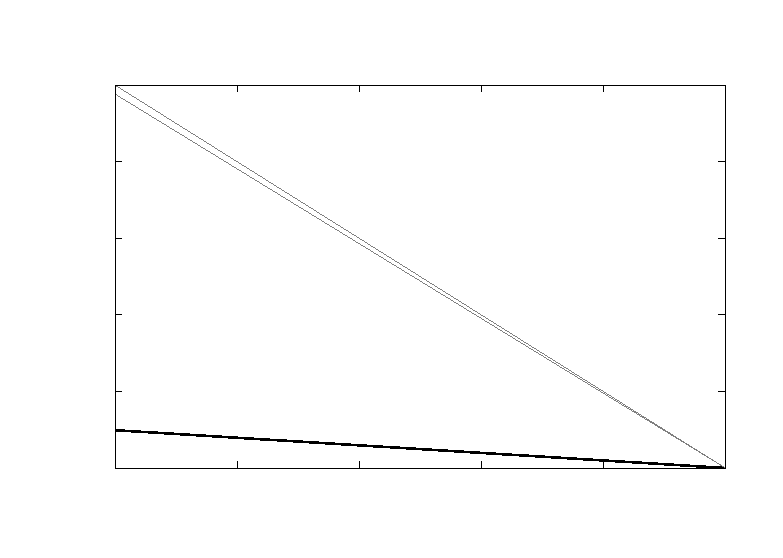
\includegraphics{gnuplot/SumConsts500Error}}%
    \gplfronttext
  \end{picture}%
\endgroup
} &
%    \scalebox{0.43}{
%      % GNUPLOT: LaTeX picture with Postscript
\begingroup
  \makeatletter
  \providecommand\color[2][]{%
    \GenericError{(gnuplot) \space\space\space\@spaces}{%
      Package color not loaded in conjunction with
      terminal option `colourtext'%
    }{See the gnuplot documentation for explanation.%
    }{Either use 'blacktext' in gnuplot or load the package
      color.sty in LaTeX.}%
    \renewcommand\color[2][]{}%
  }%
  \providecommand\includegraphics[2][]{%
    \GenericError{(gnuplot) \space\space\space\@spaces}{%
      Package graphicx or graphics not loaded%
    }{See the gnuplot documentation for explanation.%
    }{The gnuplot epslatex terminal needs graphicx.sty or graphics.sty.}%
    \renewcommand\includegraphics[2][]{}%
  }%
  \providecommand\rotatebox[2]{#2}%
  \@ifundefined{ifGPcolor}{%
    \newif\ifGPcolor
    \GPcolortrue
  }{}%
  \@ifundefined{ifGPblacktext}{%
    \newif\ifGPblacktext
    \GPblacktexttrue
  }{}%
  % define a \g@addto@macro without @ in the name:
  \let\gplgaddtomacro\g@addto@macro
  % define empty templates for all commands taking text:
  \gdef\gplbacktext{}%
  \gdef\gplfronttext{}%
  \makeatother
  \ifGPblacktext
    % no textcolor at all
    \def\colorrgb#1{}%
    \def\colorgray#1{}%
  \else
    % gray or color?
    \ifGPcolor
      \def\colorrgb#1{\color[rgb]{#1}}%
      \def\colorgray#1{\color[gray]{#1}}%
      \expandafter\def\csname LTw\endcsname{\color{white}}%
      \expandafter\def\csname LTb\endcsname{\color{black}}%
      \expandafter\def\csname LTa\endcsname{\color{black}}%
      \expandafter\def\csname LT0\endcsname{\color[rgb]{1,0,0}}%
      \expandafter\def\csname LT1\endcsname{\color[rgb]{0,1,0}}%
      \expandafter\def\csname LT2\endcsname{\color[rgb]{0,0,1}}%
      \expandafter\def\csname LT3\endcsname{\color[rgb]{1,0,1}}%
      \expandafter\def\csname LT4\endcsname{\color[rgb]{0,1,1}}%
      \expandafter\def\csname LT5\endcsname{\color[rgb]{1,1,0}}%
      \expandafter\def\csname LT6\endcsname{\color[rgb]{0,0,0}}%
      \expandafter\def\csname LT7\endcsname{\color[rgb]{1,0.3,0}}%
      \expandafter\def\csname LT8\endcsname{\color[rgb]{0.5,0.5,0.5}}%
    \else
      % gray
      \def\colorrgb#1{\color{black}}%
      \def\colorgray#1{\color[gray]{#1}}%
      \expandafter\def\csname LTw\endcsname{\color{white}}%
      \expandafter\def\csname LTb\endcsname{\color{black}}%
      \expandafter\def\csname LTa\endcsname{\color{black}}%
      \expandafter\def\csname LT0\endcsname{\color{black}}%
      \expandafter\def\csname LT1\endcsname{\color{black}}%
      \expandafter\def\csname LT2\endcsname{\color{black}}%
      \expandafter\def\csname LT3\endcsname{\color{black}}%
      \expandafter\def\csname LT4\endcsname{\color{black}}%
      \expandafter\def\csname LT5\endcsname{\color{black}}%
      \expandafter\def\csname LT6\endcsname{\color{black}}%
      \expandafter\def\csname LT7\endcsname{\color{black}}%
      \expandafter\def\csname LT8\endcsname{\color{black}}%
    \fi
  \fi
    \setlength{\unitlength}{0.0500bp}%
    \ifx\gptboxheight\undefined%
      \newlength{\gptboxheight}%
      \newlength{\gptboxwidth}%
      \newsavebox{\gptboxtext}%
    \fi%
    \setlength{\fboxrule}{0.5pt}%
    \setlength{\fboxsep}{1pt}%
\begin{picture}(7200.00,5040.00)%
    \gplgaddtomacro\gplbacktext{%
      \csname LTb\endcsname%
      \put(814,704){\makebox(0,0)[r]{\strut{}$0$}}%
      \put(814,1439){\makebox(0,0)[r]{\strut{}$0.2$}}%
      \put(814,2174){\makebox(0,0)[r]{\strut{}$0.4$}}%
      \put(814,2909){\makebox(0,0)[r]{\strut{}$0.6$}}%
      \put(814,3644){\makebox(0,0)[r]{\strut{}$0.8$}}%
      \put(814,4379){\makebox(0,0)[r]{\strut{}$1$}}%
      \put(946,484){\makebox(0,0){\strut{}$0$}}%
      \put(2117,484){\makebox(0,0){\strut{}$0.2$}}%
      \put(3289,484){\makebox(0,0){\strut{}$0.4$}}%
      \put(4460,484){\makebox(0,0){\strut{}$0.6$}}%
      \put(5632,484){\makebox(0,0){\strut{}$0.8$}}%
      \put(6803,484){\makebox(0,0){\strut{}$1$}}%
    }%
    \gplgaddtomacro\gplfronttext{%
      \csname LTb\endcsname%
      \put(176,2541){\rotatebox{-270}{\makebox(0,0){\strut{}Minimum error}}}%
      \put(3874,154){\makebox(0,0){\strut{}Generation}}%
      \put(3874,4709){\makebox(0,0){\strut{}(b) Best-of-generation error for Sum (destructive)}}%
    }%
    \gplbacktext
    \put(0,0){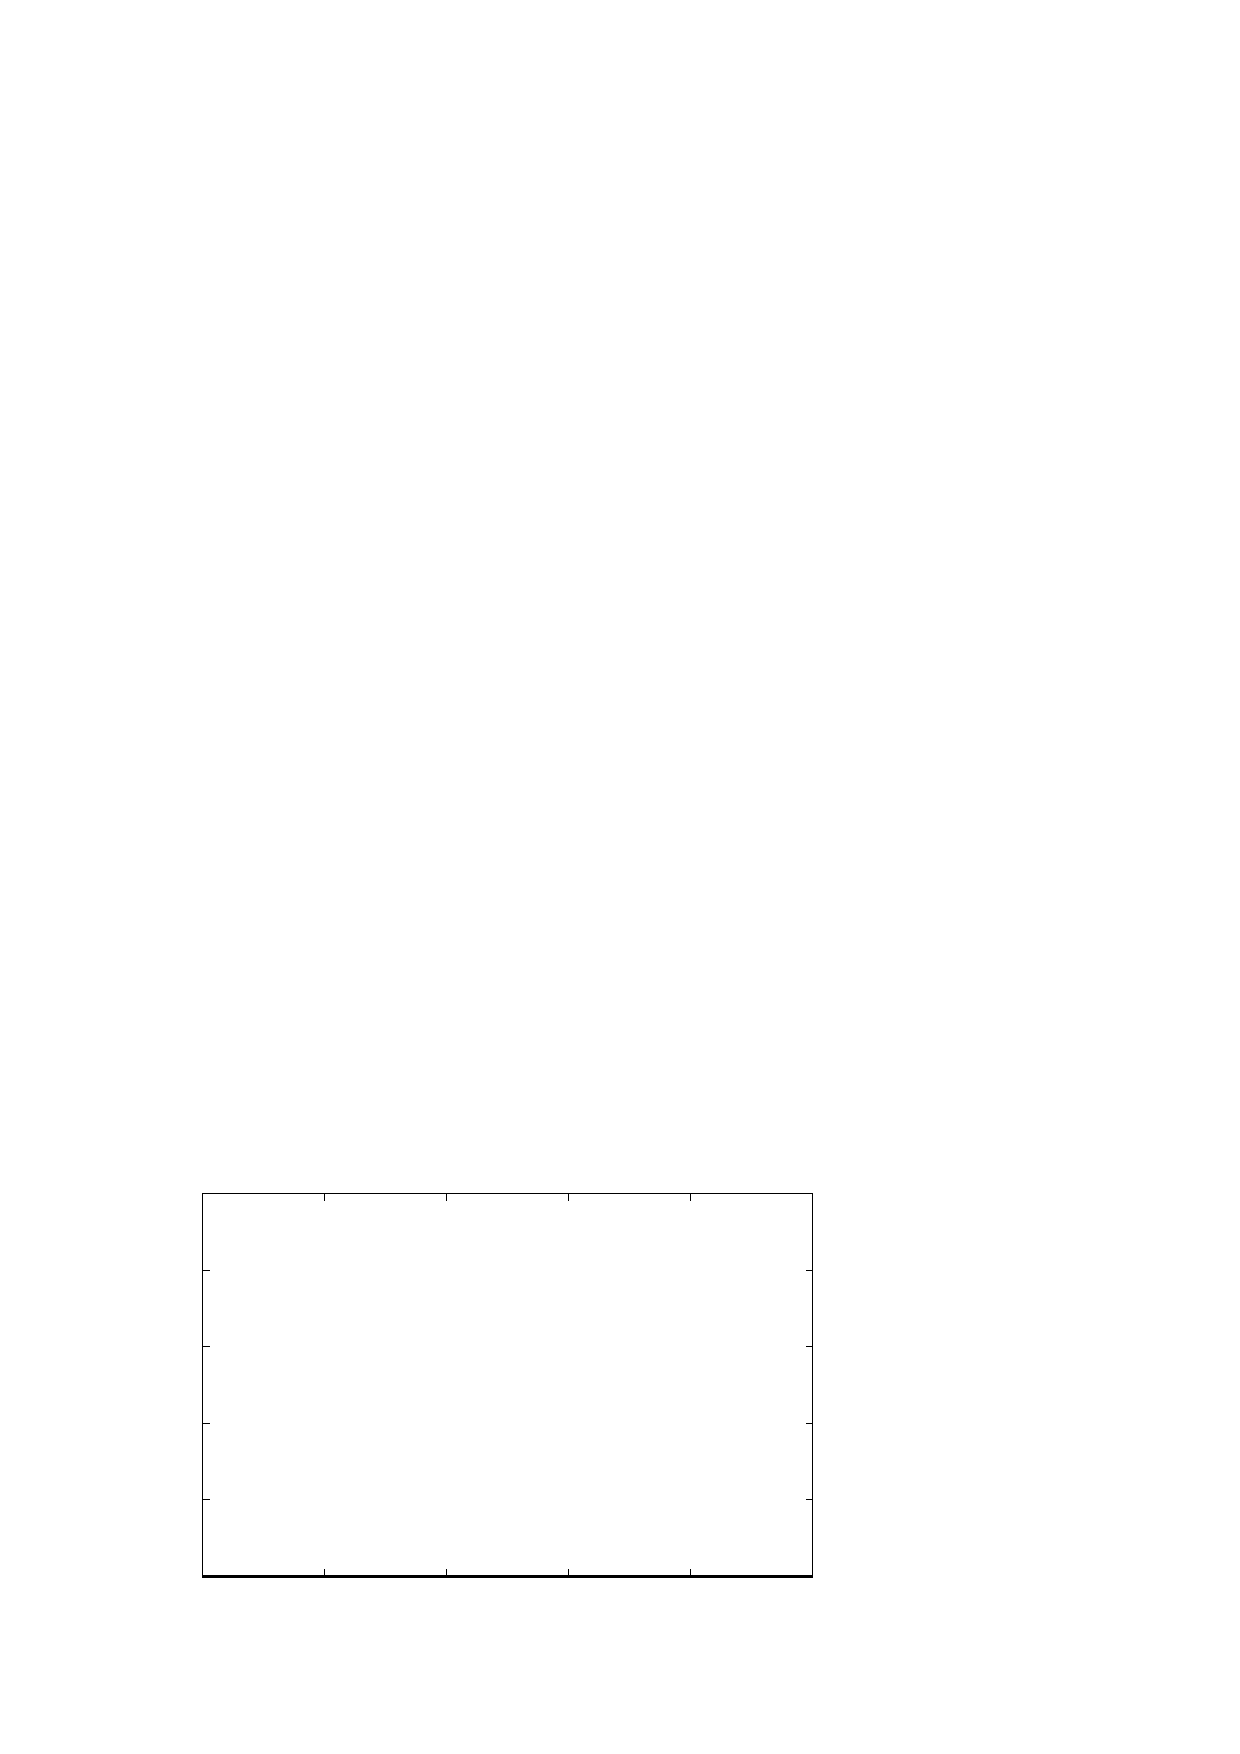
\includegraphics{gnuplot/SumDest500Error}}%
    \gplfronttext
  \end{picture}%
\endgroup
}\\
    \scalebox{0.43}{
      % GNUPLOT: LaTeX picture with Postscript
\begingroup
  \makeatletter
  \providecommand\color[2][]{%
    \GenericError{(gnuplot) \space\space\space\@spaces}{%
      Package color not loaded in conjunction with
      terminal option `colourtext'%
    }{See the gnuplot documentation for explanation.%
    }{Either use 'blacktext' in gnuplot or load the package
      color.sty in LaTeX.}%
    \renewcommand\color[2][]{}%
  }%
  \providecommand\includegraphics[2][]{%
    \GenericError{(gnuplot) \space\space\space\@spaces}{%
      Package graphicx or graphics not loaded%
    }{See the gnuplot documentation for explanation.%
    }{The gnuplot epslatex terminal needs graphicx.sty or graphics.sty.}%
    \renewcommand\includegraphics[2][]{}%
  }%
  \providecommand\rotatebox[2]{#2}%
  \@ifundefined{ifGPcolor}{%
    \newif\ifGPcolor
    \GPcolortrue
  }{}%
  \@ifundefined{ifGPblacktext}{%
    \newif\ifGPblacktext
    \GPblacktexttrue
  }{}%
  % define a \g@addto@macro without @ in the name:
  \let\gplgaddtomacro\g@addto@macro
  % define empty templates for all commands taking text:
  \gdef\gplbacktext{}%
  \gdef\gplfronttext{}%
  \makeatother
  \ifGPblacktext
    % no textcolor at all
    \def\colorrgb#1{}%
    \def\colorgray#1{}%
  \else
    % gray or color?
    \ifGPcolor
      \def\colorrgb#1{\color[rgb]{#1}}%
      \def\colorgray#1{\color[gray]{#1}}%
      \expandafter\def\csname LTw\endcsname{\color{white}}%
      \expandafter\def\csname LTb\endcsname{\color{black}}%
      \expandafter\def\csname LTa\endcsname{\color{black}}%
      \expandafter\def\csname LT0\endcsname{\color[rgb]{1,0,0}}%
      \expandafter\def\csname LT1\endcsname{\color[rgb]{0,1,0}}%
      \expandafter\def\csname LT2\endcsname{\color[rgb]{0,0,1}}%
      \expandafter\def\csname LT3\endcsname{\color[rgb]{1,0,1}}%
      \expandafter\def\csname LT4\endcsname{\color[rgb]{0,1,1}}%
      \expandafter\def\csname LT5\endcsname{\color[rgb]{1,1,0}}%
      \expandafter\def\csname LT6\endcsname{\color[rgb]{0,0,0}}%
      \expandafter\def\csname LT7\endcsname{\color[rgb]{1,0.3,0}}%
      \expandafter\def\csname LT8\endcsname{\color[rgb]{0.5,0.5,0.5}}%
    \else
      % gray
      \def\colorrgb#1{\color{black}}%
      \def\colorgray#1{\color[gray]{#1}}%
      \expandafter\def\csname LTw\endcsname{\color{white}}%
      \expandafter\def\csname LTb\endcsname{\color{black}}%
      \expandafter\def\csname LTa\endcsname{\color{black}}%
      \expandafter\def\csname LT0\endcsname{\color{black}}%
      \expandafter\def\csname LT1\endcsname{\color{black}}%
      \expandafter\def\csname LT2\endcsname{\color{black}}%
      \expandafter\def\csname LT3\endcsname{\color{black}}%
      \expandafter\def\csname LT4\endcsname{\color{black}}%
      \expandafter\def\csname LT5\endcsname{\color{black}}%
      \expandafter\def\csname LT6\endcsname{\color{black}}%
      \expandafter\def\csname LT7\endcsname{\color{black}}%
      \expandafter\def\csname LT8\endcsname{\color{black}}%
    \fi
  \fi
    \setlength{\unitlength}{0.0500bp}%
    \ifx\gptboxheight\undefined%
      \newlength{\gptboxheight}%
      \newlength{\gptboxwidth}%
      \newsavebox{\gptboxtext}%
    \fi%
    \setlength{\fboxrule}{0.5pt}%
    \setlength{\fboxsep}{1pt}%
\begin{picture}(7200.00,5040.00)%
    \gplgaddtomacro\gplbacktext{%
      \csname LTb\endcsname%
      \put(814,704){\makebox(0,0)[r]{\strut{}$0$}}%
      \put(814,1439){\makebox(0,0)[r]{\strut{}$0.2$}}%
      \put(814,2174){\makebox(0,0)[r]{\strut{}$0.4$}}%
      \put(814,2909){\makebox(0,0)[r]{\strut{}$0.6$}}%
      \put(814,3644){\makebox(0,0)[r]{\strut{}$0.8$}}%
      \put(814,4379){\makebox(0,0)[r]{\strut{}$1$}}%
      \put(946,484){\makebox(0,0){\strut{}$0$}}%
      \put(1847,484){\makebox(0,0){\strut{}$10$}}%
      \put(2748,484){\makebox(0,0){\strut{}$20$}}%
      \put(3649,484){\makebox(0,0){\strut{}$30$}}%
      \put(4550,484){\makebox(0,0){\strut{}$40$}}%
      \put(5451,484){\makebox(0,0){\strut{}$50$}}%
      \put(6352,484){\makebox(0,0){\strut{}$60$}}%
    }%
    \gplgaddtomacro\gplfronttext{%
      \csname LTb\endcsname%
      \put(176,2541){\rotatebox{-270}{\makebox(0,0){\strut{}Minimum error}}}%
      \put(3874,154){\makebox(0,0){\strut{}Generation}}%
      \put(3874,4709){\makebox(0,0){\strut{}(a) Best-of-generation error for Multiplication (constructive)}}%
    }%
    \gplbacktext
    \put(0,0){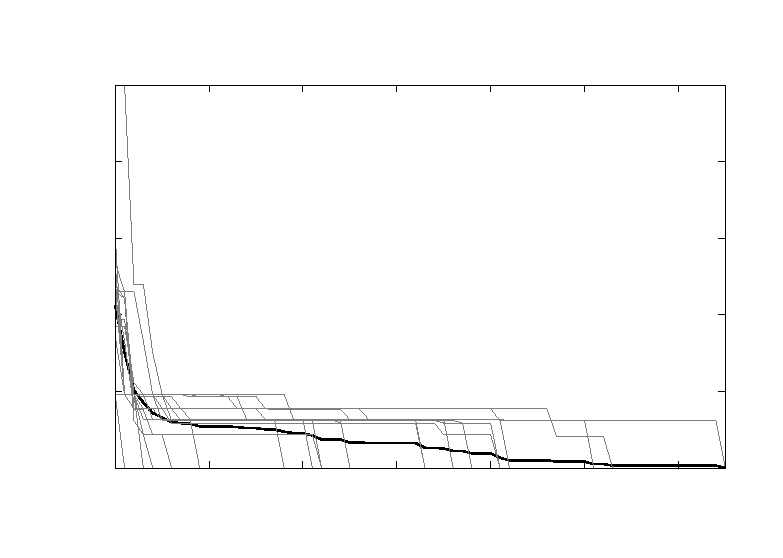
\includegraphics{gnuplot/MultiplicationConsts500Error}}%
    \gplfronttext
  \end{picture}%
\endgroup
} &
    \scalebox{0.43}{
      % GNUPLOT: LaTeX picture with Postscript
\begingroup
  \makeatletter
  \providecommand\color[2][]{%
    \GenericError{(gnuplot) \space\space\space\@spaces}{%
      Package color not loaded in conjunction with
      terminal option `colourtext'%
    }{See the gnuplot documentation for explanation.%
    }{Either use 'blacktext' in gnuplot or load the package
      color.sty in LaTeX.}%
    \renewcommand\color[2][]{}%
  }%
  \providecommand\includegraphics[2][]{%
    \GenericError{(gnuplot) \space\space\space\@spaces}{%
      Package graphicx or graphics not loaded%
    }{See the gnuplot documentation for explanation.%
    }{The gnuplot epslatex terminal needs graphicx.sty or graphics.sty.}%
    \renewcommand\includegraphics[2][]{}%
  }%
  \providecommand\rotatebox[2]{#2}%
  \@ifundefined{ifGPcolor}{%
    \newif\ifGPcolor
    \GPcolortrue
  }{}%
  \@ifundefined{ifGPblacktext}{%
    \newif\ifGPblacktext
    \GPblacktexttrue
  }{}%
  % define a \g@addto@macro without @ in the name:
  \let\gplgaddtomacro\g@addto@macro
  % define empty templates for all commands taking text:
  \gdef\gplbacktext{}%
  \gdef\gplfronttext{}%
  \makeatother
  \ifGPblacktext
    % no textcolor at all
    \def\colorrgb#1{}%
    \def\colorgray#1{}%
  \else
    % gray or color?
    \ifGPcolor
      \def\colorrgb#1{\color[rgb]{#1}}%
      \def\colorgray#1{\color[gray]{#1}}%
      \expandafter\def\csname LTw\endcsname{\color{white}}%
      \expandafter\def\csname LTb\endcsname{\color{black}}%
      \expandafter\def\csname LTa\endcsname{\color{black}}%
      \expandafter\def\csname LT0\endcsname{\color[rgb]{1,0,0}}%
      \expandafter\def\csname LT1\endcsname{\color[rgb]{0,1,0}}%
      \expandafter\def\csname LT2\endcsname{\color[rgb]{0,0,1}}%
      \expandafter\def\csname LT3\endcsname{\color[rgb]{1,0,1}}%
      \expandafter\def\csname LT4\endcsname{\color[rgb]{0,1,1}}%
      \expandafter\def\csname LT5\endcsname{\color[rgb]{1,1,0}}%
      \expandafter\def\csname LT6\endcsname{\color[rgb]{0,0,0}}%
      \expandafter\def\csname LT7\endcsname{\color[rgb]{1,0.3,0}}%
      \expandafter\def\csname LT8\endcsname{\color[rgb]{0.5,0.5,0.5}}%
    \else
      % gray
      \def\colorrgb#1{\color{black}}%
      \def\colorgray#1{\color[gray]{#1}}%
      \expandafter\def\csname LTw\endcsname{\color{white}}%
      \expandafter\def\csname LTb\endcsname{\color{black}}%
      \expandafter\def\csname LTa\endcsname{\color{black}}%
      \expandafter\def\csname LT0\endcsname{\color{black}}%
      \expandafter\def\csname LT1\endcsname{\color{black}}%
      \expandafter\def\csname LT2\endcsname{\color{black}}%
      \expandafter\def\csname LT3\endcsname{\color{black}}%
      \expandafter\def\csname LT4\endcsname{\color{black}}%
      \expandafter\def\csname LT5\endcsname{\color{black}}%
      \expandafter\def\csname LT6\endcsname{\color{black}}%
      \expandafter\def\csname LT7\endcsname{\color{black}}%
      \expandafter\def\csname LT8\endcsname{\color{black}}%
    \fi
  \fi
    \setlength{\unitlength}{0.0500bp}%
    \ifx\gptboxheight\undefined%
      \newlength{\gptboxheight}%
      \newlength{\gptboxwidth}%
      \newsavebox{\gptboxtext}%
    \fi%
    \setlength{\fboxrule}{0.5pt}%
    \setlength{\fboxsep}{1pt}%
\begin{picture}(7200.00,5040.00)%
    \gplgaddtomacro\gplbacktext{%
      \csname LTb\endcsname%
      \put(814,704){\makebox(0,0)[r]{\strut{}$0$}}%
      \put(814,1439){\makebox(0,0)[r]{\strut{}$0.2$}}%
      \put(814,2174){\makebox(0,0)[r]{\strut{}$0.4$}}%
      \put(814,2909){\makebox(0,0)[r]{\strut{}$0.6$}}%
      \put(814,3644){\makebox(0,0)[r]{\strut{}$0.8$}}%
      \put(814,4379){\makebox(0,0)[r]{\strut{}$1$}}%
      \put(946,484){\makebox(0,0){\strut{}$0$}}%
      \put(2115,484){\makebox(0,0){\strut{}$100$}}%
      \put(3284,484){\makebox(0,0){\strut{}$200$}}%
      \put(4453,484){\makebox(0,0){\strut{}$300$}}%
      \put(5622,484){\makebox(0,0){\strut{}$400$}}%
      \put(6791,484){\makebox(0,0){\strut{}$500$}}%
    }%
    \gplgaddtomacro\gplfronttext{%
      \csname LTb\endcsname%
      \put(176,2541){\rotatebox{-270}{\makebox(0,0){\strut{}Minimum error}}}%
      \put(3874,154){\makebox(0,0){\strut{}Generation}}%
      \put(3874,4709){\makebox(0,0){\strut{}(b) Best-of-generation error for Multiplication (destructive)}}%
    }%
    \gplbacktext
    \put(0,0){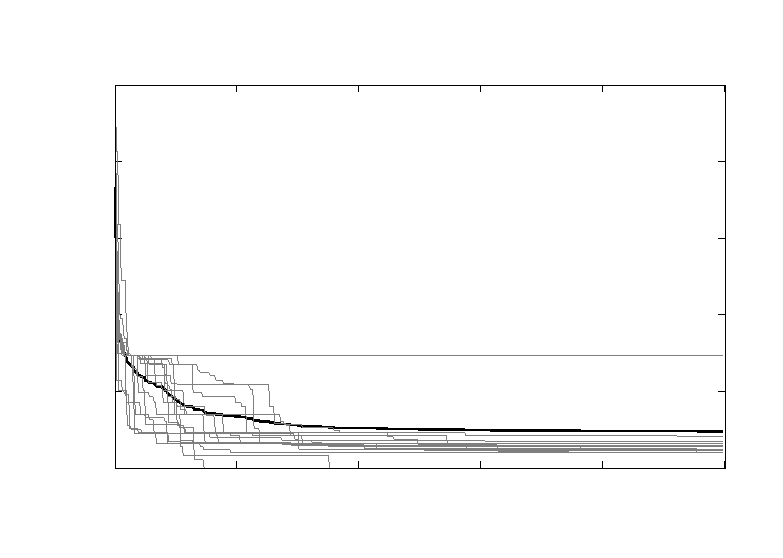
\includegraphics{gnuplot/MultiplicationDest500Error}}%
    \gplfronttext
  \end{picture}%
\endgroup
}\\
%    \scalebox{0.43}{
%      % GNUPLOT: LaTeX picture with Postscript
\begingroup
  \makeatletter
  \providecommand\color[2][]{%
    \GenericError{(gnuplot) \space\space\space\@spaces}{%
      Package color not loaded in conjunction with
      terminal option `colourtext'%
    }{See the gnuplot documentation for explanation.%
    }{Either use 'blacktext' in gnuplot or load the package
      color.sty in LaTeX.}%
    \renewcommand\color[2][]{}%
  }%
  \providecommand\includegraphics[2][]{%
    \GenericError{(gnuplot) \space\space\space\@spaces}{%
      Package graphicx or graphics not loaded%
    }{See the gnuplot documentation for explanation.%
    }{The gnuplot epslatex terminal needs graphicx.sty or graphics.sty.}%
    \renewcommand\includegraphics[2][]{}%
  }%
  \providecommand\rotatebox[2]{#2}%
  \@ifundefined{ifGPcolor}{%
    \newif\ifGPcolor
    \GPcolortrue
  }{}%
  \@ifundefined{ifGPblacktext}{%
    \newif\ifGPblacktext
    \GPblacktexttrue
  }{}%
  % define a \g@addto@macro without @ in the name:
  \let\gplgaddtomacro\g@addto@macro
  % define empty templates for all commands taking text:
  \gdef\gplbacktext{}%
  \gdef\gplfronttext{}%
  \makeatother
  \ifGPblacktext
    % no textcolor at all
    \def\colorrgb#1{}%
    \def\colorgray#1{}%
  \else
    % gray or color?
    \ifGPcolor
      \def\colorrgb#1{\color[rgb]{#1}}%
      \def\colorgray#1{\color[gray]{#1}}%
      \expandafter\def\csname LTw\endcsname{\color{white}}%
      \expandafter\def\csname LTb\endcsname{\color{black}}%
      \expandafter\def\csname LTa\endcsname{\color{black}}%
      \expandafter\def\csname LT0\endcsname{\color[rgb]{1,0,0}}%
      \expandafter\def\csname LT1\endcsname{\color[rgb]{0,1,0}}%
      \expandafter\def\csname LT2\endcsname{\color[rgb]{0,0,1}}%
      \expandafter\def\csname LT3\endcsname{\color[rgb]{1,0,1}}%
      \expandafter\def\csname LT4\endcsname{\color[rgb]{0,1,1}}%
      \expandafter\def\csname LT5\endcsname{\color[rgb]{1,1,0}}%
      \expandafter\def\csname LT6\endcsname{\color[rgb]{0,0,0}}%
      \expandafter\def\csname LT7\endcsname{\color[rgb]{1,0.3,0}}%
      \expandafter\def\csname LT8\endcsname{\color[rgb]{0.5,0.5,0.5}}%
    \else
      % gray
      \def\colorrgb#1{\color{black}}%
      \def\colorgray#1{\color[gray]{#1}}%
      \expandafter\def\csname LTw\endcsname{\color{white}}%
      \expandafter\def\csname LTb\endcsname{\color{black}}%
      \expandafter\def\csname LTa\endcsname{\color{black}}%
      \expandafter\def\csname LT0\endcsname{\color{black}}%
      \expandafter\def\csname LT1\endcsname{\color{black}}%
      \expandafter\def\csname LT2\endcsname{\color{black}}%
      \expandafter\def\csname LT3\endcsname{\color{black}}%
      \expandafter\def\csname LT4\endcsname{\color{black}}%
      \expandafter\def\csname LT5\endcsname{\color{black}}%
      \expandafter\def\csname LT6\endcsname{\color{black}}%
      \expandafter\def\csname LT7\endcsname{\color{black}}%
      \expandafter\def\csname LT8\endcsname{\color{black}}%
    \fi
  \fi
    \setlength{\unitlength}{0.0500bp}%
    \ifx\gptboxheight\undefined%
      \newlength{\gptboxheight}%
      \newlength{\gptboxwidth}%
      \newsavebox{\gptboxtext}%
    \fi%
    \setlength{\fboxrule}{0.5pt}%
    \setlength{\fboxsep}{1pt}%
\begin{picture}(7200.00,5040.00)%
    \gplgaddtomacro\gplbacktext{%
      \csname LTb\endcsname%
      \put(814,704){\makebox(0,0)[r]{\strut{}$0$}}%
      \put(814,1439){\makebox(0,0)[r]{\strut{}$0.2$}}%
      \put(814,2174){\makebox(0,0)[r]{\strut{}$0.4$}}%
      \put(814,2909){\makebox(0,0)[r]{\strut{}$0.6$}}%
      \put(814,3644){\makebox(0,0)[r]{\strut{}$0.8$}}%
      \put(814,4379){\makebox(0,0)[r]{\strut{}$1$}}%
      \put(946,484){\makebox(0,0){\strut{}$0$}}%
      \put(2117,484){\makebox(0,0){\strut{}$0.2$}}%
      \put(3289,484){\makebox(0,0){\strut{}$0.4$}}%
      \put(4460,484){\makebox(0,0){\strut{}$0.6$}}%
      \put(5632,484){\makebox(0,0){\strut{}$0.8$}}%
      \put(6803,484){\makebox(0,0){\strut{}$1$}}%
    }%
    \gplgaddtomacro\gplfronttext{%
      \csname LTb\endcsname%
      \put(176,2541){\rotatebox{-270}{\makebox(0,0){\strut{}Minimum error}}}%
      \put(3874,154){\makebox(0,0){\strut{}Generation}}%
      \put(3874,4709){\makebox(0,0){\strut{}(e) Best-of-generation error for Even/Odd (constructive)}}%
    }%
    \gplbacktext
    \put(0,0){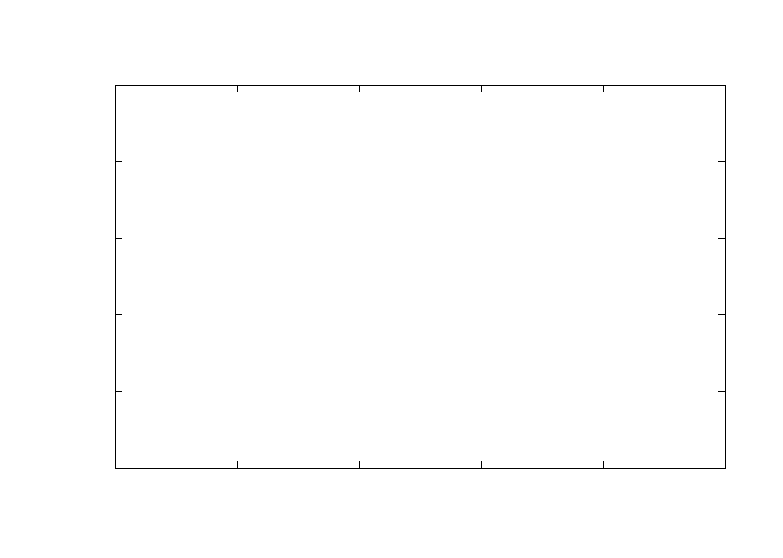
\includegraphics{gnuplot/EvenOddConsts500Error}}%
    \gplfronttext
  \end{picture}%
\endgroup
} &
%    \scalebox{0.43}{
%      % GNUPLOT: LaTeX picture with Postscript
\begingroup
  \makeatletter
  \providecommand\color[2][]{%
    \GenericError{(gnuplot) \space\space\space\@spaces}{%
      Package color not loaded in conjunction with
      terminal option `colourtext'%
    }{See the gnuplot documentation for explanation.%
    }{Either use 'blacktext' in gnuplot or load the package
      color.sty in LaTeX.}%
    \renewcommand\color[2][]{}%
  }%
  \providecommand\includegraphics[2][]{%
    \GenericError{(gnuplot) \space\space\space\@spaces}{%
      Package graphicx or graphics not loaded%
    }{See the gnuplot documentation for explanation.%
    }{The gnuplot epslatex terminal needs graphicx.sty or graphics.sty.}%
    \renewcommand\includegraphics[2][]{}%
  }%
  \providecommand\rotatebox[2]{#2}%
  \@ifundefined{ifGPcolor}{%
    \newif\ifGPcolor
    \GPcolortrue
  }{}%
  \@ifundefined{ifGPblacktext}{%
    \newif\ifGPblacktext
    \GPblacktexttrue
  }{}%
  % define a \g@addto@macro without @ in the name:
  \let\gplgaddtomacro\g@addto@macro
  % define empty templates for all commands taking text:
  \gdef\gplbacktext{}%
  \gdef\gplfronttext{}%
  \makeatother
  \ifGPblacktext
    % no textcolor at all
    \def\colorrgb#1{}%
    \def\colorgray#1{}%
  \else
    % gray or color?
    \ifGPcolor
      \def\colorrgb#1{\color[rgb]{#1}}%
      \def\colorgray#1{\color[gray]{#1}}%
      \expandafter\def\csname LTw\endcsname{\color{white}}%
      \expandafter\def\csname LTb\endcsname{\color{black}}%
      \expandafter\def\csname LTa\endcsname{\color{black}}%
      \expandafter\def\csname LT0\endcsname{\color[rgb]{1,0,0}}%
      \expandafter\def\csname LT1\endcsname{\color[rgb]{0,1,0}}%
      \expandafter\def\csname LT2\endcsname{\color[rgb]{0,0,1}}%
      \expandafter\def\csname LT3\endcsname{\color[rgb]{1,0,1}}%
      \expandafter\def\csname LT4\endcsname{\color[rgb]{0,1,1}}%
      \expandafter\def\csname LT5\endcsname{\color[rgb]{1,1,0}}%
      \expandafter\def\csname LT6\endcsname{\color[rgb]{0,0,0}}%
      \expandafter\def\csname LT7\endcsname{\color[rgb]{1,0.3,0}}%
      \expandafter\def\csname LT8\endcsname{\color[rgb]{0.5,0.5,0.5}}%
    \else
      % gray
      \def\colorrgb#1{\color{black}}%
      \def\colorgray#1{\color[gray]{#1}}%
      \expandafter\def\csname LTw\endcsname{\color{white}}%
      \expandafter\def\csname LTb\endcsname{\color{black}}%
      \expandafter\def\csname LTa\endcsname{\color{black}}%
      \expandafter\def\csname LT0\endcsname{\color{black}}%
      \expandafter\def\csname LT1\endcsname{\color{black}}%
      \expandafter\def\csname LT2\endcsname{\color{black}}%
      \expandafter\def\csname LT3\endcsname{\color{black}}%
      \expandafter\def\csname LT4\endcsname{\color{black}}%
      \expandafter\def\csname LT5\endcsname{\color{black}}%
      \expandafter\def\csname LT6\endcsname{\color{black}}%
      \expandafter\def\csname LT7\endcsname{\color{black}}%
      \expandafter\def\csname LT8\endcsname{\color{black}}%
    \fi
  \fi
    \setlength{\unitlength}{0.0500bp}%
    \ifx\gptboxheight\undefined%
      \newlength{\gptboxheight}%
      \newlength{\gptboxwidth}%
      \newsavebox{\gptboxtext}%
    \fi%
    \setlength{\fboxrule}{0.5pt}%
    \setlength{\fboxsep}{1pt}%
\begin{picture}(7200.00,5040.00)%
    \gplgaddtomacro\gplbacktext{%
      \csname LTb\endcsname%
      \put(814,704){\makebox(0,0)[r]{\strut{}$0$}}%
      \put(814,1439){\makebox(0,0)[r]{\strut{}$0.2$}}%
      \put(814,2174){\makebox(0,0)[r]{\strut{}$0.4$}}%
      \put(814,2909){\makebox(0,0)[r]{\strut{}$0.6$}}%
      \put(814,3644){\makebox(0,0)[r]{\strut{}$0.8$}}%
      \put(814,4379){\makebox(0,0)[r]{\strut{}$1$}}%
      \put(946,484){\makebox(0,0){\strut{}$0$}}%
      \put(1727,484){\makebox(0,0){\strut{}$2$}}%
      \put(2508,484){\makebox(0,0){\strut{}$4$}}%
      \put(3289,484){\makebox(0,0){\strut{}$6$}}%
      \put(4070,484){\makebox(0,0){\strut{}$8$}}%
      \put(4851,484){\makebox(0,0){\strut{}$10$}}%
      \put(5632,484){\makebox(0,0){\strut{}$12$}}%
      \put(6413,484){\makebox(0,0){\strut{}$14$}}%
    }%
    \gplgaddtomacro\gplfronttext{%
      \csname LTb\endcsname%
      \put(176,2541){\rotatebox{-270}{\makebox(0,0){\strut{}Minimum error}}}%
      \put(3874,154){\makebox(0,0){\strut{}Generation}}%
      \put(3874,4709){\makebox(0,0){\strut{}(f) Best-of-generation error for Even/Odd (destructive)}}%
    }%
    \gplbacktext
    \put(0,0){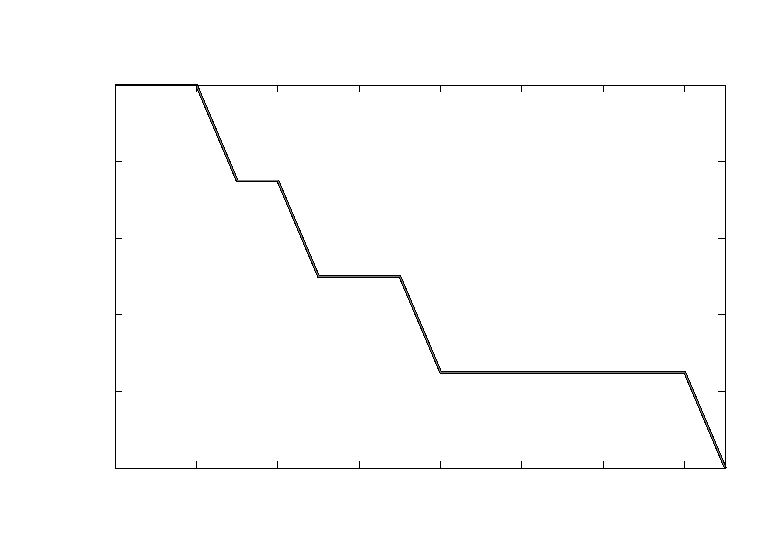
\includegraphics{gnuplot/EvenOddDest500Error}}%
    \gplfronttext
  \end{picture}%
\endgroup
}\\
    \scalebox{0.43}{
      % GNUPLOT: LaTeX picture with Postscript
\begingroup
  \makeatletter
  \providecommand\color[2][]{%
    \GenericError{(gnuplot) \space\space\space\@spaces}{%
      Package color not loaded in conjunction with
      terminal option `colourtext'%
    }{See the gnuplot documentation for explanation.%
    }{Either use 'blacktext' in gnuplot or load the package
      color.sty in LaTeX.}%
    \renewcommand\color[2][]{}%
  }%
  \providecommand\includegraphics[2][]{%
    \GenericError{(gnuplot) \space\space\space\@spaces}{%
      Package graphicx or graphics not loaded%
    }{See the gnuplot documentation for explanation.%
    }{The gnuplot epslatex terminal needs graphicx.sty or graphics.sty.}%
    \renewcommand\includegraphics[2][]{}%
  }%
  \providecommand\rotatebox[2]{#2}%
  \@ifundefined{ifGPcolor}{%
    \newif\ifGPcolor
    \GPcolortrue
  }{}%
  \@ifundefined{ifGPblacktext}{%
    \newif\ifGPblacktext
    \GPblacktexttrue
  }{}%
  % define a \g@addto@macro without @ in the name:
  \let\gplgaddtomacro\g@addto@macro
  % define empty templates for all commands taking text:
  \gdef\gplbacktext{}%
  \gdef\gplfronttext{}%
  \makeatother
  \ifGPblacktext
    % no textcolor at all
    \def\colorrgb#1{}%
    \def\colorgray#1{}%
  \else
    % gray or color?
    \ifGPcolor
      \def\colorrgb#1{\color[rgb]{#1}}%
      \def\colorgray#1{\color[gray]{#1}}%
      \expandafter\def\csname LTw\endcsname{\color{white}}%
      \expandafter\def\csname LTb\endcsname{\color{black}}%
      \expandafter\def\csname LTa\endcsname{\color{black}}%
      \expandafter\def\csname LT0\endcsname{\color[rgb]{1,0,0}}%
      \expandafter\def\csname LT1\endcsname{\color[rgb]{0,1,0}}%
      \expandafter\def\csname LT2\endcsname{\color[rgb]{0,0,1}}%
      \expandafter\def\csname LT3\endcsname{\color[rgb]{1,0,1}}%
      \expandafter\def\csname LT4\endcsname{\color[rgb]{0,1,1}}%
      \expandafter\def\csname LT5\endcsname{\color[rgb]{1,1,0}}%
      \expandafter\def\csname LT6\endcsname{\color[rgb]{0,0,0}}%
      \expandafter\def\csname LT7\endcsname{\color[rgb]{1,0.3,0}}%
      \expandafter\def\csname LT8\endcsname{\color[rgb]{0.5,0.5,0.5}}%
    \else
      % gray
      \def\colorrgb#1{\color{black}}%
      \def\colorgray#1{\color[gray]{#1}}%
      \expandafter\def\csname LTw\endcsname{\color{white}}%
      \expandafter\def\csname LTb\endcsname{\color{black}}%
      \expandafter\def\csname LTa\endcsname{\color{black}}%
      \expandafter\def\csname LT0\endcsname{\color{black}}%
      \expandafter\def\csname LT1\endcsname{\color{black}}%
      \expandafter\def\csname LT2\endcsname{\color{black}}%
      \expandafter\def\csname LT3\endcsname{\color{black}}%
      \expandafter\def\csname LT4\endcsname{\color{black}}%
      \expandafter\def\csname LT5\endcsname{\color{black}}%
      \expandafter\def\csname LT6\endcsname{\color{black}}%
      \expandafter\def\csname LT7\endcsname{\color{black}}%
      \expandafter\def\csname LT8\endcsname{\color{black}}%
    \fi
  \fi
    \setlength{\unitlength}{0.0500bp}%
    \ifx\gptboxheight\undefined%
      \newlength{\gptboxheight}%
      \newlength{\gptboxwidth}%
      \newsavebox{\gptboxtext}%
    \fi%
    \setlength{\fboxrule}{0.5pt}%
    \setlength{\fboxsep}{1pt}%
\begin{picture}(7200.00,5040.00)%
    \gplgaddtomacro\gplbacktext{%
      \csname LTb\endcsname%
      \put(814,704){\makebox(0,0)[r]{\strut{}$0$}}%
      \put(814,1439){\makebox(0,0)[r]{\strut{}$0.2$}}%
      \put(814,2174){\makebox(0,0)[r]{\strut{}$0.4$}}%
      \put(814,2909){\makebox(0,0)[r]{\strut{}$0.6$}}%
      \put(814,3644){\makebox(0,0)[r]{\strut{}$0.8$}}%
      \put(814,4379){\makebox(0,0)[r]{\strut{}$1$}}%
      \put(946,484){\makebox(0,0){\strut{}$0$}}%
      \put(1697,484){\makebox(0,0){\strut{}$5$}}%
      \put(2448,484){\makebox(0,0){\strut{}$10$}}%
      \put(3199,484){\makebox(0,0){\strut{}$15$}}%
      \put(3950,484){\makebox(0,0){\strut{}$20$}}%
      \put(4700,484){\makebox(0,0){\strut{}$25$}}%
      \put(5451,484){\makebox(0,0){\strut{}$30$}}%
      \put(6202,484){\makebox(0,0){\strut{}$35$}}%
    }%
    \gplgaddtomacro\gplfronttext{%
      \csname LTb\endcsname%
      \put(176,2541){\rotatebox{-270}{\makebox(0,0){\strut{}Minimum error}}}%
      \put(3874,154){\makebox(0,0){\strut{}Generation}}%
      \put(3874,4709){\makebox(0,0){\strut{}(c) Best-of-generation error for Ackermann (constructive)}}%
    }%
    \gplbacktext
    \put(0,0){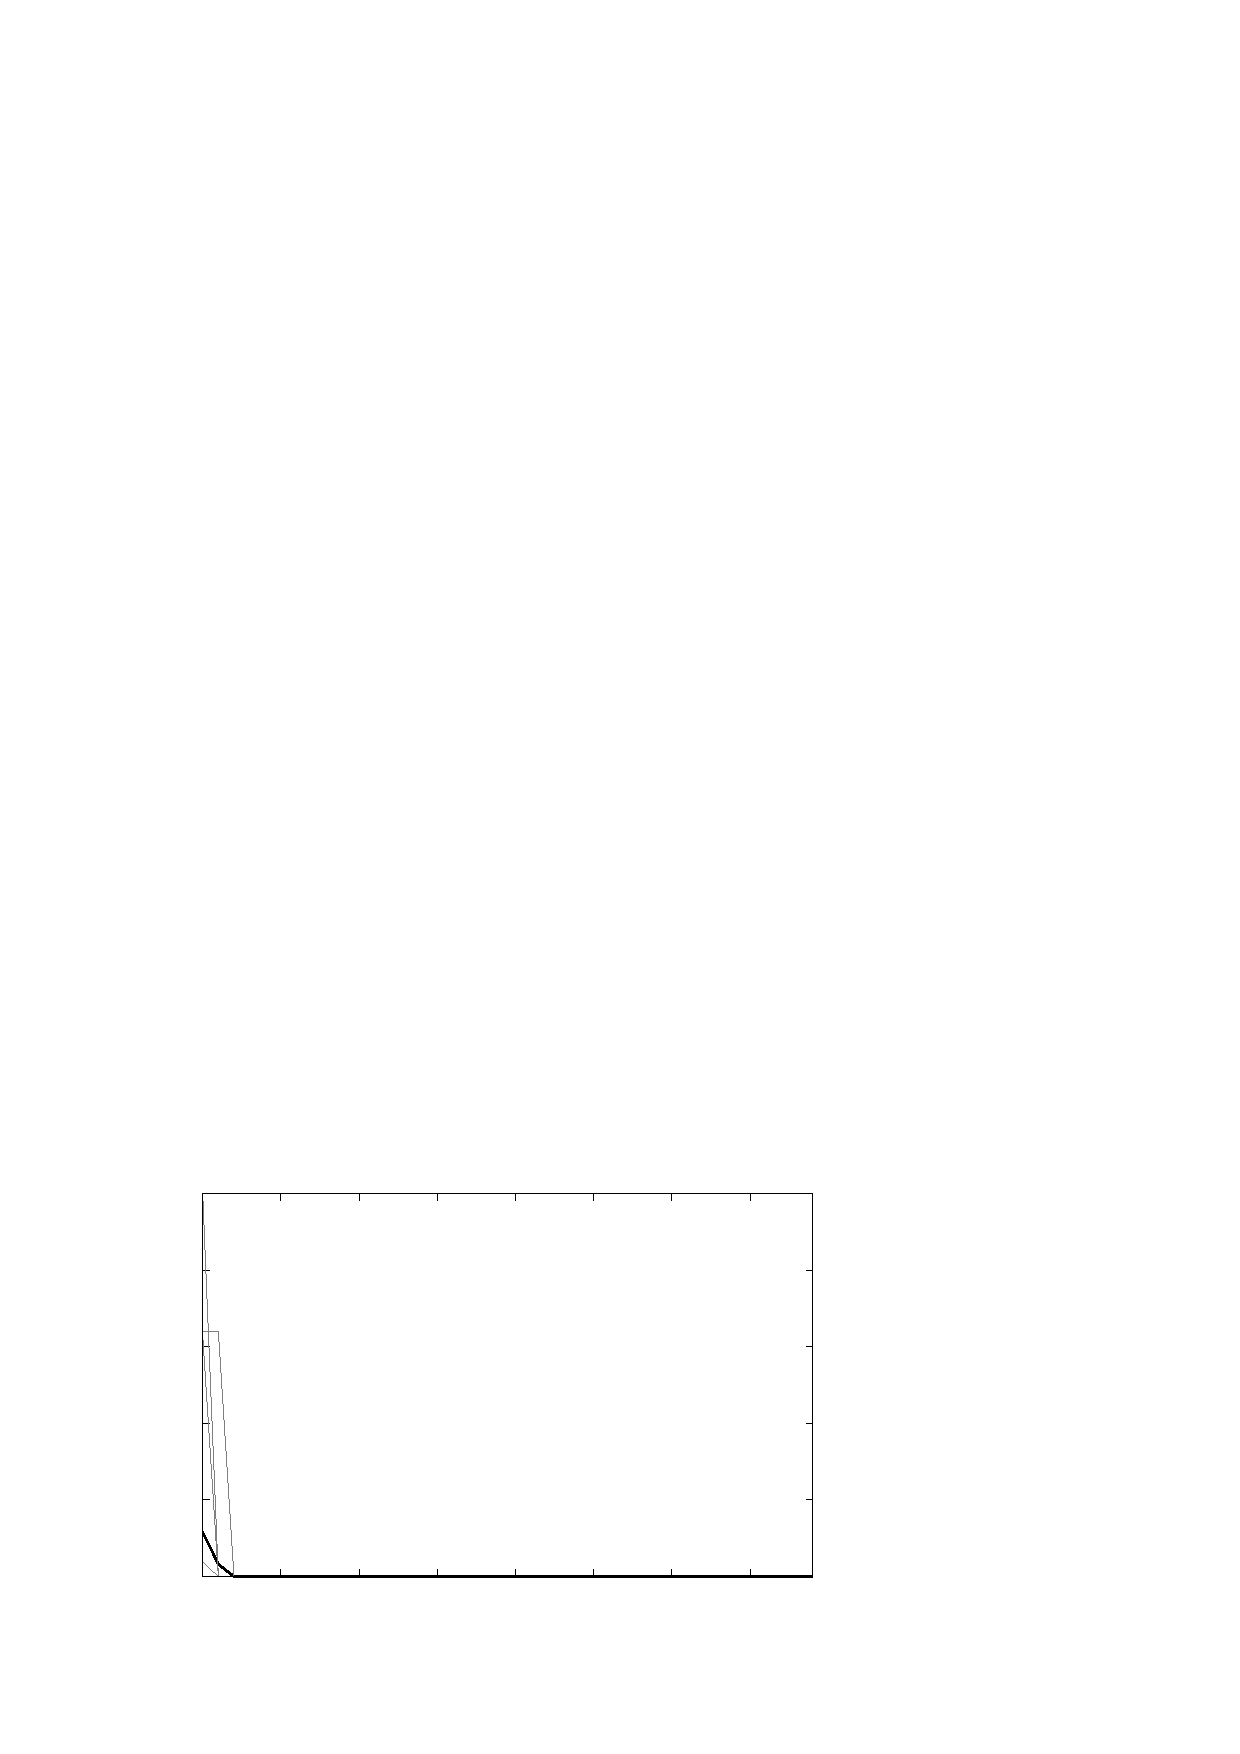
\includegraphics{gnuplot/AckermannConsts500Error}}%
    \gplfronttext
  \end{picture}%
\endgroup
} &
    \scalebox{0.43}{
      % GNUPLOT: LaTeX picture with Postscript
\begingroup
  \makeatletter
  \providecommand\color[2][]{%
    \GenericError{(gnuplot) \space\space\space\@spaces}{%
      Package color not loaded in conjunction with
      terminal option `colourtext'%
    }{See the gnuplot documentation for explanation.%
    }{Either use 'blacktext' in gnuplot or load the package
      color.sty in LaTeX.}%
    \renewcommand\color[2][]{}%
  }%
  \providecommand\includegraphics[2][]{%
    \GenericError{(gnuplot) \space\space\space\@spaces}{%
      Package graphicx or graphics not loaded%
    }{See the gnuplot documentation for explanation.%
    }{The gnuplot epslatex terminal needs graphicx.sty or graphics.sty.}%
    \renewcommand\includegraphics[2][]{}%
  }%
  \providecommand\rotatebox[2]{#2}%
  \@ifundefined{ifGPcolor}{%
    \newif\ifGPcolor
    \GPcolortrue
  }{}%
  \@ifundefined{ifGPblacktext}{%
    \newif\ifGPblacktext
    \GPblacktexttrue
  }{}%
  % define a \g@addto@macro without @ in the name:
  \let\gplgaddtomacro\g@addto@macro
  % define empty templates for all commands taking text:
  \gdef\gplbacktext{}%
  \gdef\gplfronttext{}%
  \makeatother
  \ifGPblacktext
    % no textcolor at all
    \def\colorrgb#1{}%
    \def\colorgray#1{}%
  \else
    % gray or color?
    \ifGPcolor
      \def\colorrgb#1{\color[rgb]{#1}}%
      \def\colorgray#1{\color[gray]{#1}}%
      \expandafter\def\csname LTw\endcsname{\color{white}}%
      \expandafter\def\csname LTb\endcsname{\color{black}}%
      \expandafter\def\csname LTa\endcsname{\color{black}}%
      \expandafter\def\csname LT0\endcsname{\color[rgb]{1,0,0}}%
      \expandafter\def\csname LT1\endcsname{\color[rgb]{0,1,0}}%
      \expandafter\def\csname LT2\endcsname{\color[rgb]{0,0,1}}%
      \expandafter\def\csname LT3\endcsname{\color[rgb]{1,0,1}}%
      \expandafter\def\csname LT4\endcsname{\color[rgb]{0,1,1}}%
      \expandafter\def\csname LT5\endcsname{\color[rgb]{1,1,0}}%
      \expandafter\def\csname LT6\endcsname{\color[rgb]{0,0,0}}%
      \expandafter\def\csname LT7\endcsname{\color[rgb]{1,0.3,0}}%
      \expandafter\def\csname LT8\endcsname{\color[rgb]{0.5,0.5,0.5}}%
    \else
      % gray
      \def\colorrgb#1{\color{black}}%
      \def\colorgray#1{\color[gray]{#1}}%
      \expandafter\def\csname LTw\endcsname{\color{white}}%
      \expandafter\def\csname LTb\endcsname{\color{black}}%
      \expandafter\def\csname LTa\endcsname{\color{black}}%
      \expandafter\def\csname LT0\endcsname{\color{black}}%
      \expandafter\def\csname LT1\endcsname{\color{black}}%
      \expandafter\def\csname LT2\endcsname{\color{black}}%
      \expandafter\def\csname LT3\endcsname{\color{black}}%
      \expandafter\def\csname LT4\endcsname{\color{black}}%
      \expandafter\def\csname LT5\endcsname{\color{black}}%
      \expandafter\def\csname LT6\endcsname{\color{black}}%
      \expandafter\def\csname LT7\endcsname{\color{black}}%
      \expandafter\def\csname LT8\endcsname{\color{black}}%
    \fi
  \fi
    \setlength{\unitlength}{0.0500bp}%
    \ifx\gptboxheight\undefined%
      \newlength{\gptboxheight}%
      \newlength{\gptboxwidth}%
      \newsavebox{\gptboxtext}%
    \fi%
    \setlength{\fboxrule}{0.5pt}%
    \setlength{\fboxsep}{1pt}%
\begin{picture}(7200.00,5040.00)%
    \gplgaddtomacro\gplbacktext{%
      \csname LTb\endcsname%
      \put(814,704){\makebox(0,0)[r]{\strut{}$0$}}%
      \put(814,1439){\makebox(0,0)[r]{\strut{}$0.2$}}%
      \put(814,2174){\makebox(0,0)[r]{\strut{}$0.4$}}%
      \put(814,2909){\makebox(0,0)[r]{\strut{}$0.6$}}%
      \put(814,3644){\makebox(0,0)[r]{\strut{}$0.8$}}%
      \put(814,4379){\makebox(0,0)[r]{\strut{}$1$}}%
      \put(946,484){\makebox(0,0){\strut{}$0$}}%
      \put(2115,484){\makebox(0,0){\strut{}$100$}}%
      \put(3284,484){\makebox(0,0){\strut{}$200$}}%
      \put(4453,484){\makebox(0,0){\strut{}$300$}}%
      \put(5622,484){\makebox(0,0){\strut{}$400$}}%
      \put(6791,484){\makebox(0,0){\strut{}$500$}}%
    }%
    \gplgaddtomacro\gplfronttext{%
      \csname LTb\endcsname%
      \put(176,2541){\rotatebox{-270}{\makebox(0,0){\strut{}Minimum error}}}%
      \put(3874,154){\makebox(0,0){\strut{}Generation}}%
      \put(3874,4709){\makebox(0,0){\strut{}(d) Best-of-generation error for Ackermann (destructive)}}%
    }%
    \gplbacktext
    \put(0,0){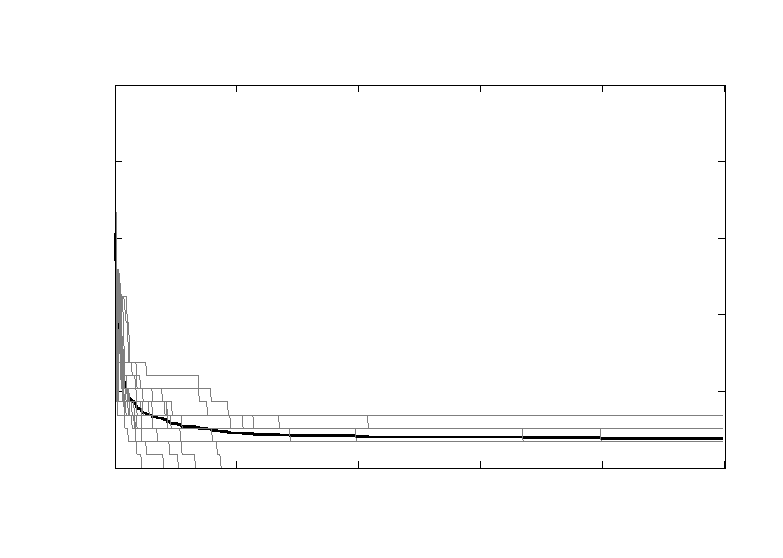
\includegraphics{gnuplot/AckermannDest500Error}}%
    \gplfronttext
  \end{picture}%
\endgroup
}
  \end{tabular}
  \caption{Best-of-generation error graphs for the two search regimes of case studies.}
  \label{fig:error}
\end{figure}

\begin{figure}[!ht]
  \begin{tabular}{cc}
%    \scalebox{0.43}{
%      % GNUPLOT: LaTeX picture with Postscript
\begingroup
  \makeatletter
  \providecommand\color[2][]{%
    \GenericError{(gnuplot) \space\space\space\@spaces}{%
      Package color not loaded in conjunction with
      terminal option `colourtext'%
    }{See the gnuplot documentation for explanation.%
    }{Either use 'blacktext' in gnuplot or load the package
      color.sty in LaTeX.}%
    \renewcommand\color[2][]{}%
  }%
  \providecommand\includegraphics[2][]{%
    \GenericError{(gnuplot) \space\space\space\@spaces}{%
      Package graphicx or graphics not loaded%
    }{See the gnuplot documentation for explanation.%
    }{The gnuplot epslatex terminal needs graphicx.sty or graphics.sty.}%
    \renewcommand\includegraphics[2][]{}%
  }%
  \providecommand\rotatebox[2]{#2}%
  \@ifundefined{ifGPcolor}{%
    \newif\ifGPcolor
    \GPcolortrue
  }{}%
  \@ifundefined{ifGPblacktext}{%
    \newif\ifGPblacktext
    \GPblacktexttrue
  }{}%
  % define a \g@addto@macro without @ in the name:
  \let\gplgaddtomacro\g@addto@macro
  % define empty templates for all commands taking text:
  \gdef\gplbacktext{}%
  \gdef\gplfronttext{}%
  \makeatother
  \ifGPblacktext
    % no textcolor at all
    \def\colorrgb#1{}%
    \def\colorgray#1{}%
  \else
    % gray or color?
    \ifGPcolor
      \def\colorrgb#1{\color[rgb]{#1}}%
      \def\colorgray#1{\color[gray]{#1}}%
      \expandafter\def\csname LTw\endcsname{\color{white}}%
      \expandafter\def\csname LTb\endcsname{\color{black}}%
      \expandafter\def\csname LTa\endcsname{\color{black}}%
      \expandafter\def\csname LT0\endcsname{\color[rgb]{1,0,0}}%
      \expandafter\def\csname LT1\endcsname{\color[rgb]{0,1,0}}%
      \expandafter\def\csname LT2\endcsname{\color[rgb]{0,0,1}}%
      \expandafter\def\csname LT3\endcsname{\color[rgb]{1,0,1}}%
      \expandafter\def\csname LT4\endcsname{\color[rgb]{0,1,1}}%
      \expandafter\def\csname LT5\endcsname{\color[rgb]{1,1,0}}%
      \expandafter\def\csname LT6\endcsname{\color[rgb]{0,0,0}}%
      \expandafter\def\csname LT7\endcsname{\color[rgb]{1,0.3,0}}%
      \expandafter\def\csname LT8\endcsname{\color[rgb]{0.5,0.5,0.5}}%
    \else
      % gray
      \def\colorrgb#1{\color{black}}%
      \def\colorgray#1{\color[gray]{#1}}%
      \expandafter\def\csname LTw\endcsname{\color{white}}%
      \expandafter\def\csname LTb\endcsname{\color{black}}%
      \expandafter\def\csname LTa\endcsname{\color{black}}%
      \expandafter\def\csname LT0\endcsname{\color{black}}%
      \expandafter\def\csname LT1\endcsname{\color{black}}%
      \expandafter\def\csname LT2\endcsname{\color{black}}%
      \expandafter\def\csname LT3\endcsname{\color{black}}%
      \expandafter\def\csname LT4\endcsname{\color{black}}%
      \expandafter\def\csname LT5\endcsname{\color{black}}%
      \expandafter\def\csname LT6\endcsname{\color{black}}%
      \expandafter\def\csname LT7\endcsname{\color{black}}%
      \expandafter\def\csname LT8\endcsname{\color{black}}%
    \fi
  \fi
    \setlength{\unitlength}{0.0500bp}%
    \ifx\gptboxheight\undefined%
      \newlength{\gptboxheight}%
      \newlength{\gptboxwidth}%
      \newsavebox{\gptboxtext}%
    \fi%
    \setlength{\fboxrule}{0.5pt}%
    \setlength{\fboxsep}{1pt}%
\begin{picture}(7200.00,5040.00)%
    \gplgaddtomacro\gplbacktext{%
      \csname LTb\endcsname%
      \put(814,704){\makebox(0,0)[r]{\strut{}$0$}}%
      \put(814,1439){\makebox(0,0)[r]{\strut{}$0.2$}}%
      \put(814,2174){\makebox(0,0)[r]{\strut{}$0.4$}}%
      \put(814,2909){\makebox(0,0)[r]{\strut{}$0.6$}}%
      \put(814,3644){\makebox(0,0)[r]{\strut{}$0.8$}}%
      \put(814,4379){\makebox(0,0)[r]{\strut{}$1$}}%
      \put(946,484){\makebox(0,0){\strut{}$0$}}%
      \put(2117,484){\makebox(0,0){\strut{}$100$}}%
      \put(3289,484){\makebox(0,0){\strut{}$200$}}%
      \put(4460,484){\makebox(0,0){\strut{}$300$}}%
      \put(5632,484){\makebox(0,0){\strut{}$400$}}%
      \put(6803,484){\makebox(0,0){\strut{}$500$}}%
    }%
    \gplgaddtomacro\gplfronttext{%
      \csname LTb\endcsname%
      \put(176,2541){\rotatebox{-270}{\makebox(0,0){\strut{}CPS}}}%
      \put(3874,154){\makebox(0,0){\strut{}Generation}}%
      \put(3874,4709){\makebox(0,0){\strut{}(a) Cumulative Probability of Success for Sum}}%
      \csname LTb\endcsname%
      \put(5816,4206){\makebox(0,0)[r]{\strut{}Constructive}}%
      \csname LTb\endcsname%
      \put(5816,3986){\makebox(0,0)[r]{\strut{}Destructive}}%
    }%
    \gplbacktext
    \put(0,0){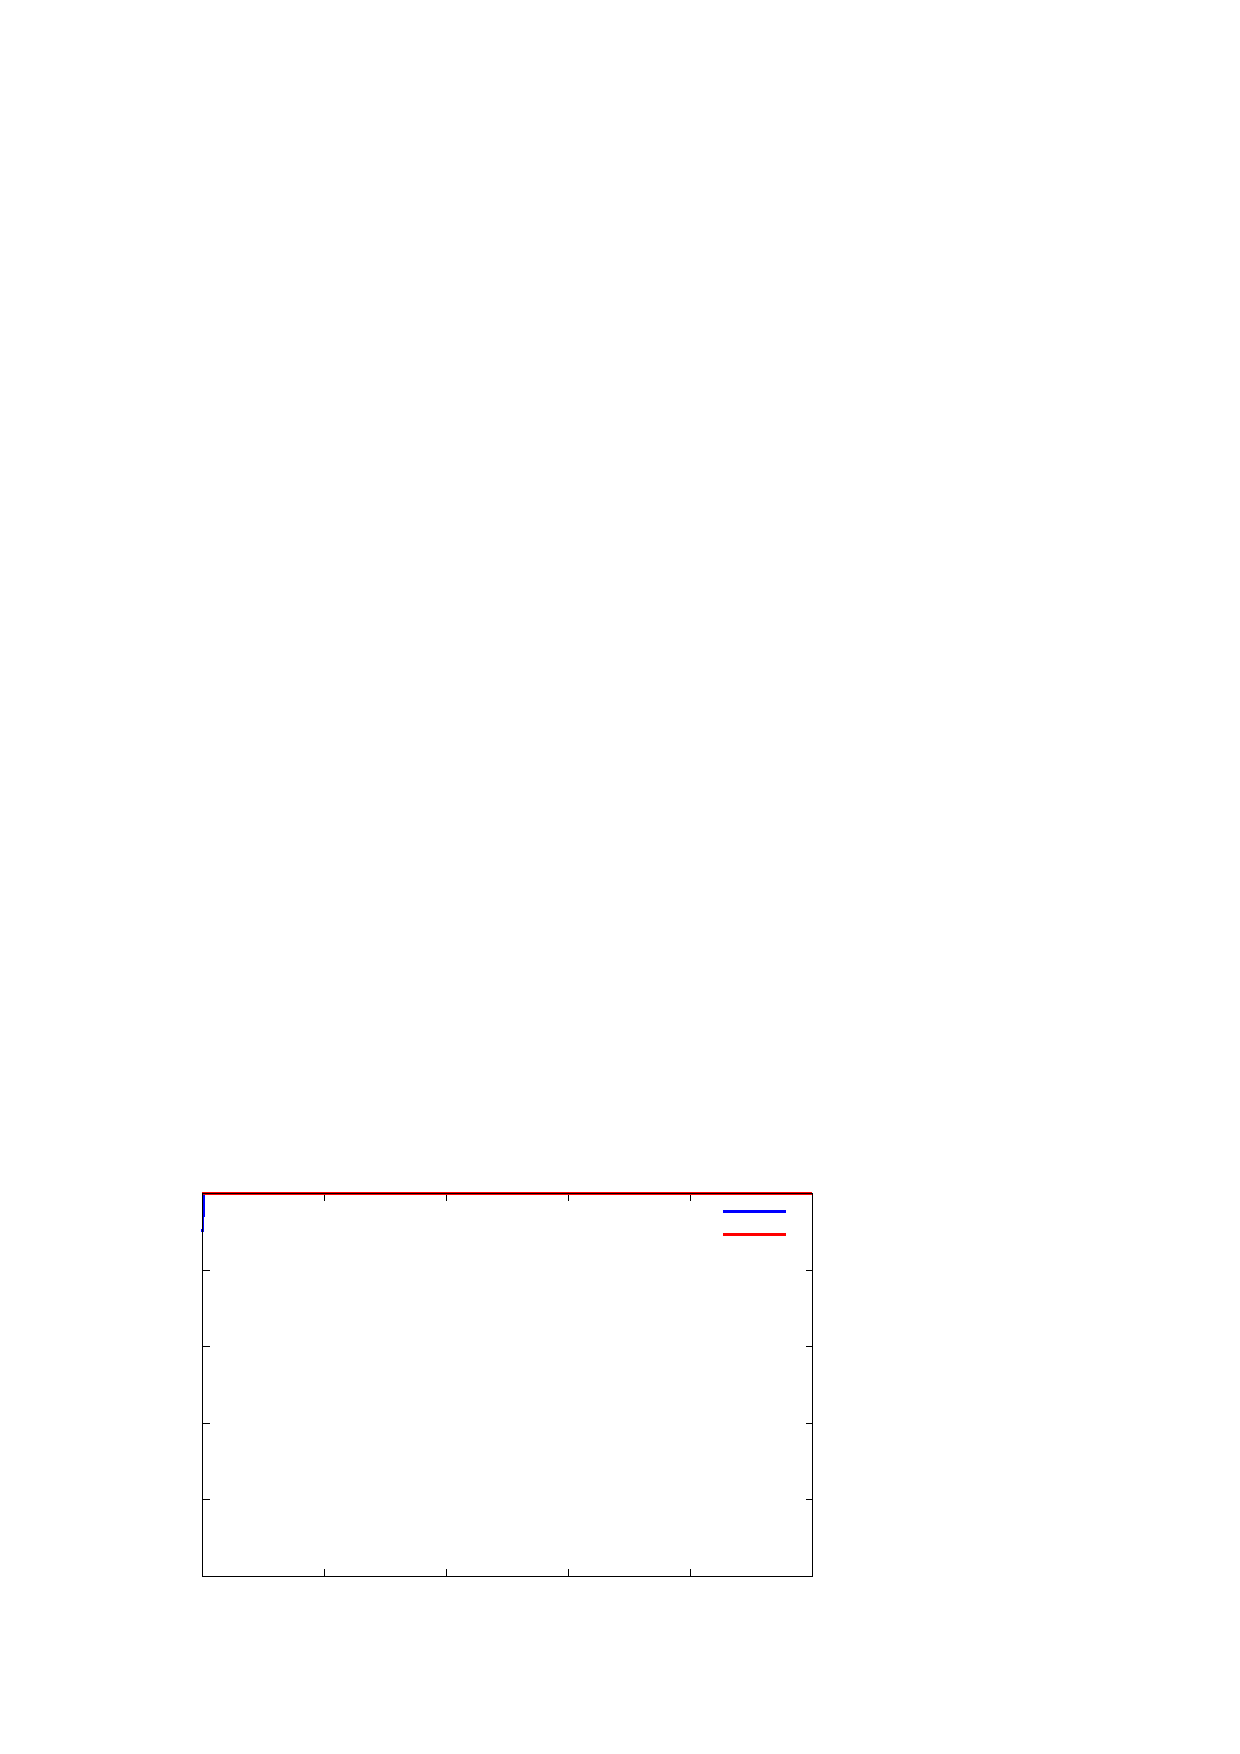
\includegraphics{gnuplot/Sum500Cumulative}}%
    \gplfronttext
  \end{picture}%
\endgroup
} &
    \scalebox{0.43}{
      % GNUPLOT: LaTeX picture with Postscript
\begingroup
  \makeatletter
  \providecommand\color[2][]{%
    \GenericError{(gnuplot) \space\space\space\@spaces}{%
      Package color not loaded in conjunction with
      terminal option `colourtext'%
    }{See the gnuplot documentation for explanation.%
    }{Either use 'blacktext' in gnuplot or load the package
      color.sty in LaTeX.}%
    \renewcommand\color[2][]{}%
  }%
  \providecommand\includegraphics[2][]{%
    \GenericError{(gnuplot) \space\space\space\@spaces}{%
      Package graphicx or graphics not loaded%
    }{See the gnuplot documentation for explanation.%
    }{The gnuplot epslatex terminal needs graphicx.sty or graphics.sty.}%
    \renewcommand\includegraphics[2][]{}%
  }%
  \providecommand\rotatebox[2]{#2}%
  \@ifundefined{ifGPcolor}{%
    \newif\ifGPcolor
    \GPcolortrue
  }{}%
  \@ifundefined{ifGPblacktext}{%
    \newif\ifGPblacktext
    \GPblacktexttrue
  }{}%
  % define a \g@addto@macro without @ in the name:
  \let\gplgaddtomacro\g@addto@macro
  % define empty templates for all commands taking text:
  \gdef\gplbacktext{}%
  \gdef\gplfronttext{}%
  \makeatother
  \ifGPblacktext
    % no textcolor at all
    \def\colorrgb#1{}%
    \def\colorgray#1{}%
  \else
    % gray or color?
    \ifGPcolor
      \def\colorrgb#1{\color[rgb]{#1}}%
      \def\colorgray#1{\color[gray]{#1}}%
      \expandafter\def\csname LTw\endcsname{\color{white}}%
      \expandafter\def\csname LTb\endcsname{\color{black}}%
      \expandafter\def\csname LTa\endcsname{\color{black}}%
      \expandafter\def\csname LT0\endcsname{\color[rgb]{1,0,0}}%
      \expandafter\def\csname LT1\endcsname{\color[rgb]{0,1,0}}%
      \expandafter\def\csname LT2\endcsname{\color[rgb]{0,0,1}}%
      \expandafter\def\csname LT3\endcsname{\color[rgb]{1,0,1}}%
      \expandafter\def\csname LT4\endcsname{\color[rgb]{0,1,1}}%
      \expandafter\def\csname LT5\endcsname{\color[rgb]{1,1,0}}%
      \expandafter\def\csname LT6\endcsname{\color[rgb]{0,0,0}}%
      \expandafter\def\csname LT7\endcsname{\color[rgb]{1,0.3,0}}%
      \expandafter\def\csname LT8\endcsname{\color[rgb]{0.5,0.5,0.5}}%
    \else
      % gray
      \def\colorrgb#1{\color{black}}%
      \def\colorgray#1{\color[gray]{#1}}%
      \expandafter\def\csname LTw\endcsname{\color{white}}%
      \expandafter\def\csname LTb\endcsname{\color{black}}%
      \expandafter\def\csname LTa\endcsname{\color{black}}%
      \expandafter\def\csname LT0\endcsname{\color{black}}%
      \expandafter\def\csname LT1\endcsname{\color{black}}%
      \expandafter\def\csname LT2\endcsname{\color{black}}%
      \expandafter\def\csname LT3\endcsname{\color{black}}%
      \expandafter\def\csname LT4\endcsname{\color{black}}%
      \expandafter\def\csname LT5\endcsname{\color{black}}%
      \expandafter\def\csname LT6\endcsname{\color{black}}%
      \expandafter\def\csname LT7\endcsname{\color{black}}%
      \expandafter\def\csname LT8\endcsname{\color{black}}%
    \fi
  \fi
    \setlength{\unitlength}{0.0500bp}%
    \ifx\gptboxheight\undefined%
      \newlength{\gptboxheight}%
      \newlength{\gptboxwidth}%
      \newsavebox{\gptboxtext}%
    \fi%
    \setlength{\fboxrule}{0.5pt}%
    \setlength{\fboxsep}{1pt}%
\begin{picture}(7200.00,5040.00)%
    \gplgaddtomacro\gplbacktext{%
      \csname LTb\endcsname%
      \put(814,704){\makebox(0,0)[r]{\strut{}$0$}}%
      \put(814,1439){\makebox(0,0)[r]{\strut{}$0.2$}}%
      \put(814,2174){\makebox(0,0)[r]{\strut{}$0.4$}}%
      \put(814,2909){\makebox(0,0)[r]{\strut{}$0.6$}}%
      \put(814,3644){\makebox(0,0)[r]{\strut{}$0.8$}}%
      \put(814,4379){\makebox(0,0)[r]{\strut{}$1$}}%
      \put(946,484){\makebox(0,0){\strut{}$0$}}%
      \put(2117,484){\makebox(0,0){\strut{}$100$}}%
      \put(3289,484){\makebox(0,0){\strut{}$200$}}%
      \put(4460,484){\makebox(0,0){\strut{}$300$}}%
      \put(5632,484){\makebox(0,0){\strut{}$400$}}%
      \put(6803,484){\makebox(0,0){\strut{}$500$}}%
    }%
    \gplgaddtomacro\gplfronttext{%
      \csname LTb\endcsname%
      \put(176,2541){\rotatebox{-270}{\makebox(0,0){\strut{}CPS}}}%
      \put(3874,154){\makebox(0,0){\strut{}Generation}}%
      \put(3874,4709){\makebox(0,0){\strut{}(a) Cumulative Probability of Success for Multiplication}}%
      \csname LTb\endcsname%
      \put(5816,4206){\makebox(0,0)[r]{\strut{}Constructive}}%
      \csname LTb\endcsname%
      \put(5816,3986){\makebox(0,0)[r]{\strut{}Destructive}}%
    }%
    \gplbacktext
    \put(0,0){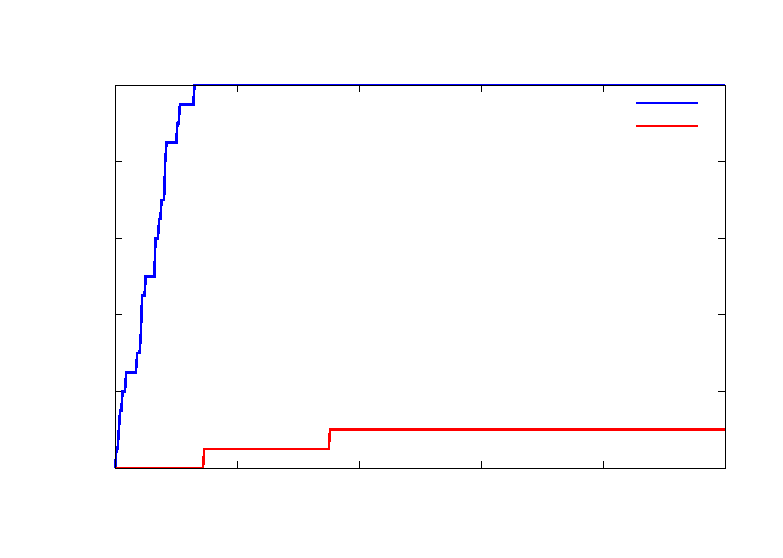
\includegraphics{gnuplot/Multiplication500Cumulative}}%
    \gplfronttext
  \end{picture}%
\endgroup
} &
%    \scalebox{0.43}{
%      % GNUPLOT: LaTeX picture with Postscript
\begingroup
  \makeatletter
  \providecommand\color[2][]{%
    \GenericError{(gnuplot) \space\space\space\@spaces}{%
      Package color not loaded in conjunction with
      terminal option `colourtext'%
    }{See the gnuplot documentation for explanation.%
    }{Either use 'blacktext' in gnuplot or load the package
      color.sty in LaTeX.}%
    \renewcommand\color[2][]{}%
  }%
  \providecommand\includegraphics[2][]{%
    \GenericError{(gnuplot) \space\space\space\@spaces}{%
      Package graphicx or graphics not loaded%
    }{See the gnuplot documentation for explanation.%
    }{The gnuplot epslatex terminal needs graphicx.sty or graphics.sty.}%
    \renewcommand\includegraphics[2][]{}%
  }%
  \providecommand\rotatebox[2]{#2}%
  \@ifundefined{ifGPcolor}{%
    \newif\ifGPcolor
    \GPcolortrue
  }{}%
  \@ifundefined{ifGPblacktext}{%
    \newif\ifGPblacktext
    \GPblacktexttrue
  }{}%
  % define a \g@addto@macro without @ in the name:
  \let\gplgaddtomacro\g@addto@macro
  % define empty templates for all commands taking text:
  \gdef\gplbacktext{}%
  \gdef\gplfronttext{}%
  \makeatother
  \ifGPblacktext
    % no textcolor at all
    \def\colorrgb#1{}%
    \def\colorgray#1{}%
  \else
    % gray or color?
    \ifGPcolor
      \def\colorrgb#1{\color[rgb]{#1}}%
      \def\colorgray#1{\color[gray]{#1}}%
      \expandafter\def\csname LTw\endcsname{\color{white}}%
      \expandafter\def\csname LTb\endcsname{\color{black}}%
      \expandafter\def\csname LTa\endcsname{\color{black}}%
      \expandafter\def\csname LT0\endcsname{\color[rgb]{1,0,0}}%
      \expandafter\def\csname LT1\endcsname{\color[rgb]{0,1,0}}%
      \expandafter\def\csname LT2\endcsname{\color[rgb]{0,0,1}}%
      \expandafter\def\csname LT3\endcsname{\color[rgb]{1,0,1}}%
      \expandafter\def\csname LT4\endcsname{\color[rgb]{0,1,1}}%
      \expandafter\def\csname LT5\endcsname{\color[rgb]{1,1,0}}%
      \expandafter\def\csname LT6\endcsname{\color[rgb]{0,0,0}}%
      \expandafter\def\csname LT7\endcsname{\color[rgb]{1,0.3,0}}%
      \expandafter\def\csname LT8\endcsname{\color[rgb]{0.5,0.5,0.5}}%
    \else
      % gray
      \def\colorrgb#1{\color{black}}%
      \def\colorgray#1{\color[gray]{#1}}%
      \expandafter\def\csname LTw\endcsname{\color{white}}%
      \expandafter\def\csname LTb\endcsname{\color{black}}%
      \expandafter\def\csname LTa\endcsname{\color{black}}%
      \expandafter\def\csname LT0\endcsname{\color{black}}%
      \expandafter\def\csname LT1\endcsname{\color{black}}%
      \expandafter\def\csname LT2\endcsname{\color{black}}%
      \expandafter\def\csname LT3\endcsname{\color{black}}%
      \expandafter\def\csname LT4\endcsname{\color{black}}%
      \expandafter\def\csname LT5\endcsname{\color{black}}%
      \expandafter\def\csname LT6\endcsname{\color{black}}%
      \expandafter\def\csname LT7\endcsname{\color{black}}%
      \expandafter\def\csname LT8\endcsname{\color{black}}%
    \fi
  \fi
    \setlength{\unitlength}{0.0500bp}%
    \ifx\gptboxheight\undefined%
      \newlength{\gptboxheight}%
      \newlength{\gptboxwidth}%
      \newsavebox{\gptboxtext}%
    \fi%
    \setlength{\fboxrule}{0.5pt}%
    \setlength{\fboxsep}{1pt}%
\begin{picture}(7200.00,5040.00)%
    \gplgaddtomacro\gplbacktext{%
      \csname LTb\endcsname%
      \put(814,704){\makebox(0,0)[r]{\strut{}$0$}}%
      \put(814,1439){\makebox(0,0)[r]{\strut{}$0.2$}}%
      \put(814,2174){\makebox(0,0)[r]{\strut{}$0.4$}}%
      \put(814,2909){\makebox(0,0)[r]{\strut{}$0.6$}}%
      \put(814,3644){\makebox(0,0)[r]{\strut{}$0.8$}}%
      \put(814,4379){\makebox(0,0)[r]{\strut{}$1$}}%
      \put(946,484){\makebox(0,0){\strut{}$0$}}%
      \put(2117,484){\makebox(0,0){\strut{}$100$}}%
      \put(3289,484){\makebox(0,0){\strut{}$200$}}%
      \put(4460,484){\makebox(0,0){\strut{}$300$}}%
      \put(5632,484){\makebox(0,0){\strut{}$400$}}%
      \put(6803,484){\makebox(0,0){\strut{}$500$}}%
    }%
    \gplgaddtomacro\gplfronttext{%
      \csname LTb\endcsname%
      \put(176,2541){\rotatebox{-270}{\makebox(0,0){\strut{}CPS}}}%
      \put(3874,154){\makebox(0,0){\strut{}Generation}}%
      \put(3874,4709){\makebox(0,0){\strut{}(c) Cumulative Probability of Success for Even/Odd}}%
      \csname LTb\endcsname%
      \put(5816,4206){\makebox(0,0)[r]{\strut{}Constructive}}%
      \csname LTb\endcsname%
      \put(5816,3986){\makebox(0,0)[r]{\strut{}Destructive}}%
    }%
    \gplbacktext
    \put(0,0){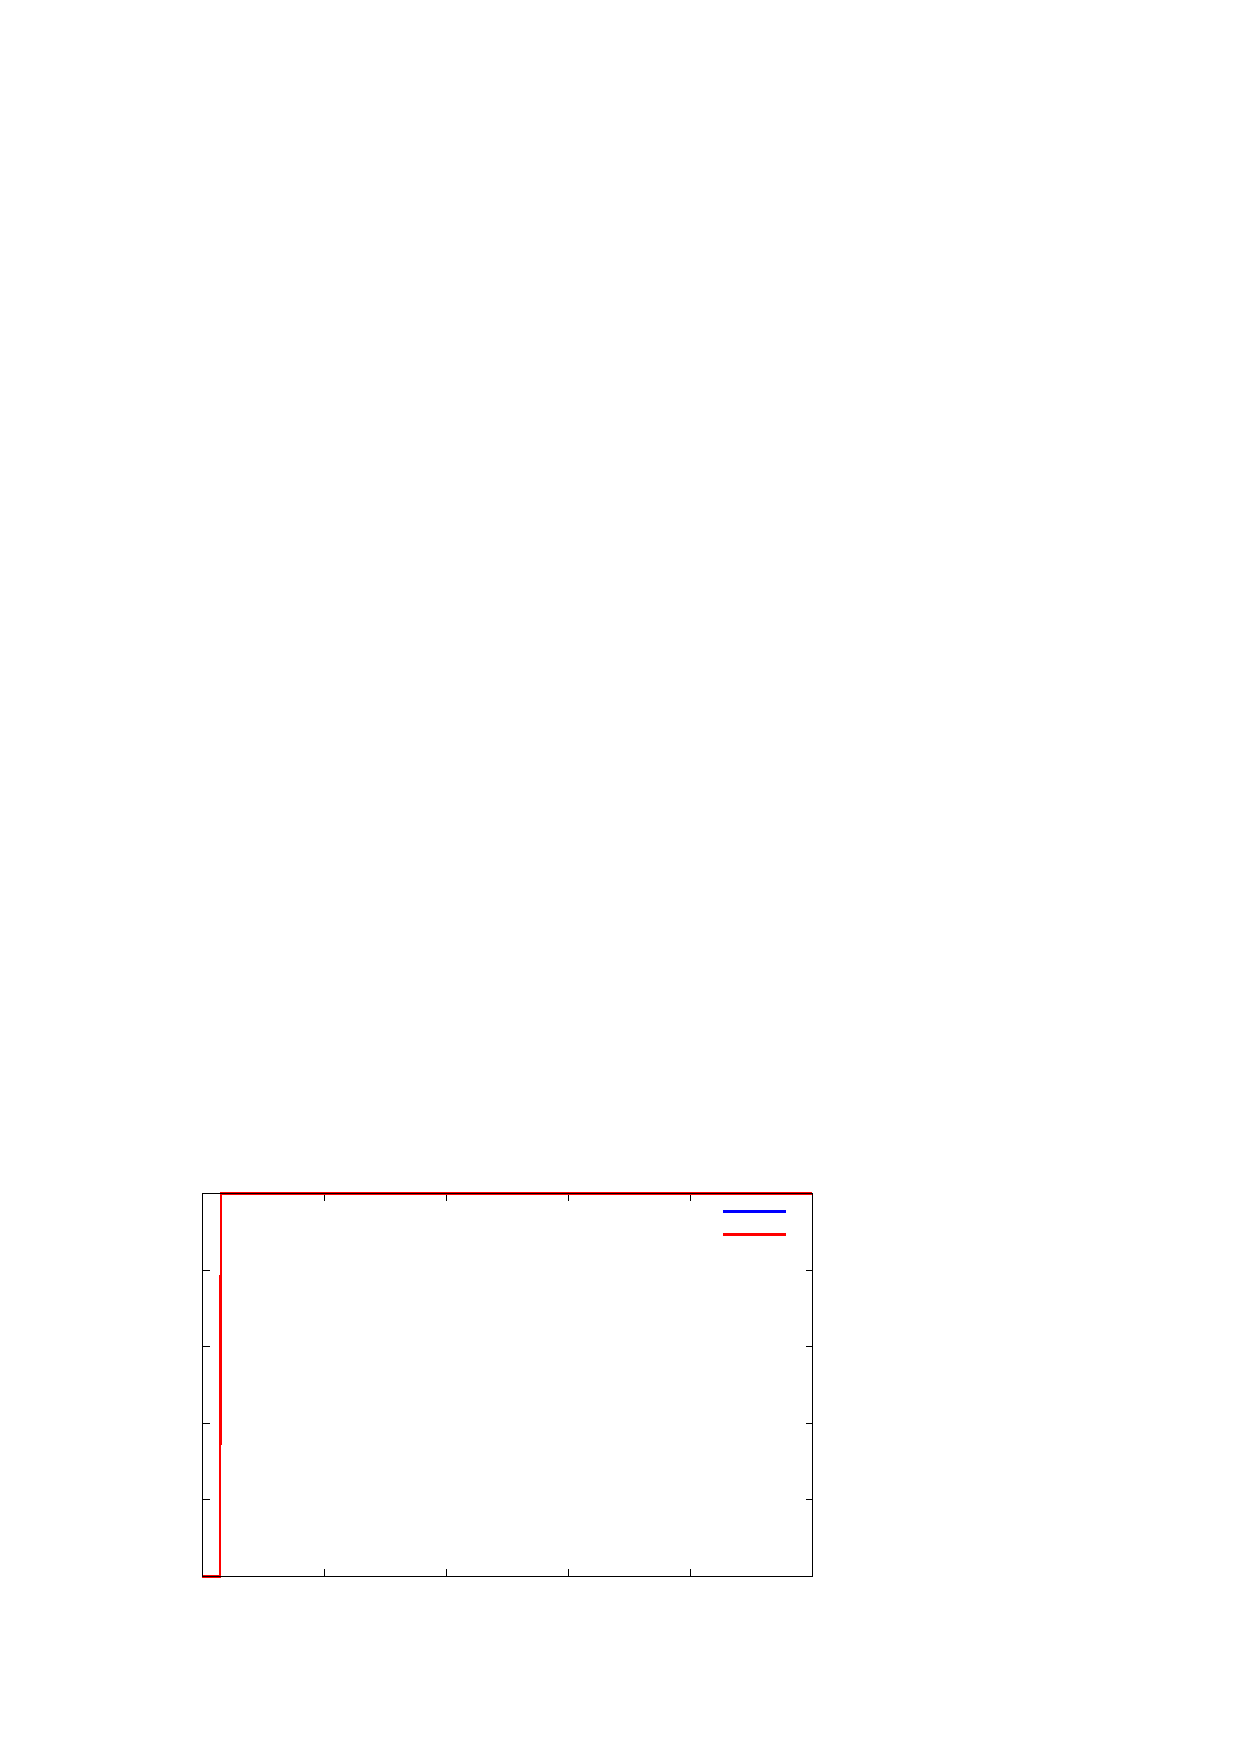
\includegraphics{gnuplot/EvenOdd500Cumulative}}%
    \gplfronttext
  \end{picture}%
\endgroup
} &
    \scalebox{0.43}{
      % GNUPLOT: LaTeX picture with Postscript
\begingroup
  \makeatletter
  \providecommand\color[2][]{%
    \GenericError{(gnuplot) \space\space\space\@spaces}{%
      Package color not loaded in conjunction with
      terminal option `colourtext'%
    }{See the gnuplot documentation for explanation.%
    }{Either use 'blacktext' in gnuplot or load the package
      color.sty in LaTeX.}%
    \renewcommand\color[2][]{}%
  }%
  \providecommand\includegraphics[2][]{%
    \GenericError{(gnuplot) \space\space\space\@spaces}{%
      Package graphicx or graphics not loaded%
    }{See the gnuplot documentation for explanation.%
    }{The gnuplot epslatex terminal needs graphicx.sty or graphics.sty.}%
    \renewcommand\includegraphics[2][]{}%
  }%
  \providecommand\rotatebox[2]{#2}%
  \@ifundefined{ifGPcolor}{%
    \newif\ifGPcolor
    \GPcolortrue
  }{}%
  \@ifundefined{ifGPblacktext}{%
    \newif\ifGPblacktext
    \GPblacktexttrue
  }{}%
  % define a \g@addto@macro without @ in the name:
  \let\gplgaddtomacro\g@addto@macro
  % define empty templates for all commands taking text:
  \gdef\gplbacktext{}%
  \gdef\gplfronttext{}%
  \makeatother
  \ifGPblacktext
    % no textcolor at all
    \def\colorrgb#1{}%
    \def\colorgray#1{}%
  \else
    % gray or color?
    \ifGPcolor
      \def\colorrgb#1{\color[rgb]{#1}}%
      \def\colorgray#1{\color[gray]{#1}}%
      \expandafter\def\csname LTw\endcsname{\color{white}}%
      \expandafter\def\csname LTb\endcsname{\color{black}}%
      \expandafter\def\csname LTa\endcsname{\color{black}}%
      \expandafter\def\csname LT0\endcsname{\color[rgb]{1,0,0}}%
      \expandafter\def\csname LT1\endcsname{\color[rgb]{0,1,0}}%
      \expandafter\def\csname LT2\endcsname{\color[rgb]{0,0,1}}%
      \expandafter\def\csname LT3\endcsname{\color[rgb]{1,0,1}}%
      \expandafter\def\csname LT4\endcsname{\color[rgb]{0,1,1}}%
      \expandafter\def\csname LT5\endcsname{\color[rgb]{1,1,0}}%
      \expandafter\def\csname LT6\endcsname{\color[rgb]{0,0,0}}%
      \expandafter\def\csname LT7\endcsname{\color[rgb]{1,0.3,0}}%
      \expandafter\def\csname LT8\endcsname{\color[rgb]{0.5,0.5,0.5}}%
    \else
      % gray
      \def\colorrgb#1{\color{black}}%
      \def\colorgray#1{\color[gray]{#1}}%
      \expandafter\def\csname LTw\endcsname{\color{white}}%
      \expandafter\def\csname LTb\endcsname{\color{black}}%
      \expandafter\def\csname LTa\endcsname{\color{black}}%
      \expandafter\def\csname LT0\endcsname{\color{black}}%
      \expandafter\def\csname LT1\endcsname{\color{black}}%
      \expandafter\def\csname LT2\endcsname{\color{black}}%
      \expandafter\def\csname LT3\endcsname{\color{black}}%
      \expandafter\def\csname LT4\endcsname{\color{black}}%
      \expandafter\def\csname LT5\endcsname{\color{black}}%
      \expandafter\def\csname LT6\endcsname{\color{black}}%
      \expandafter\def\csname LT7\endcsname{\color{black}}%
      \expandafter\def\csname LT8\endcsname{\color{black}}%
    \fi
  \fi
    \setlength{\unitlength}{0.0500bp}%
    \ifx\gptboxheight\undefined%
      \newlength{\gptboxheight}%
      \newlength{\gptboxwidth}%
      \newsavebox{\gptboxtext}%
    \fi%
    \setlength{\fboxrule}{0.5pt}%
    \setlength{\fboxsep}{1pt}%
\begin{picture}(7200.00,5040.00)%
    \gplgaddtomacro\gplbacktext{%
      \csname LTb\endcsname%
      \put(814,704){\makebox(0,0)[r]{\strut{}$0$}}%
      \put(814,1439){\makebox(0,0)[r]{\strut{}$0.2$}}%
      \put(814,2174){\makebox(0,0)[r]{\strut{}$0.4$}}%
      \put(814,2909){\makebox(0,0)[r]{\strut{}$0.6$}}%
      \put(814,3644){\makebox(0,0)[r]{\strut{}$0.8$}}%
      \put(814,4379){\makebox(0,0)[r]{\strut{}$1$}}%
      \put(946,484){\makebox(0,0){\strut{}$0$}}%
      \put(2117,484){\makebox(0,0){\strut{}$100$}}%
      \put(3289,484){\makebox(0,0){\strut{}$200$}}%
      \put(4460,484){\makebox(0,0){\strut{}$300$}}%
      \put(5632,484){\makebox(0,0){\strut{}$400$}}%
      \put(6803,484){\makebox(0,0){\strut{}$500$}}%
    }%
    \gplgaddtomacro\gplfronttext{%
      \csname LTb\endcsname%
      \put(176,2541){\rotatebox{-270}{\makebox(0,0){\strut{}CPS}}}%
      \put(3874,154){\makebox(0,0){\strut{}Generation}}%
      \put(3874,4709){\makebox(0,0){\strut{}(b) Cumulative Probability of Success for Ackermann}}%
      \csname LTb\endcsname%
      \put(5816,4206){\makebox(0,0)[r]{\strut{}Constructive}}%
      \csname LTb\endcsname%
      \put(5816,3986){\makebox(0,0)[r]{\strut{}Destructive}}%
    }%
    \gplbacktext
    \put(0,0){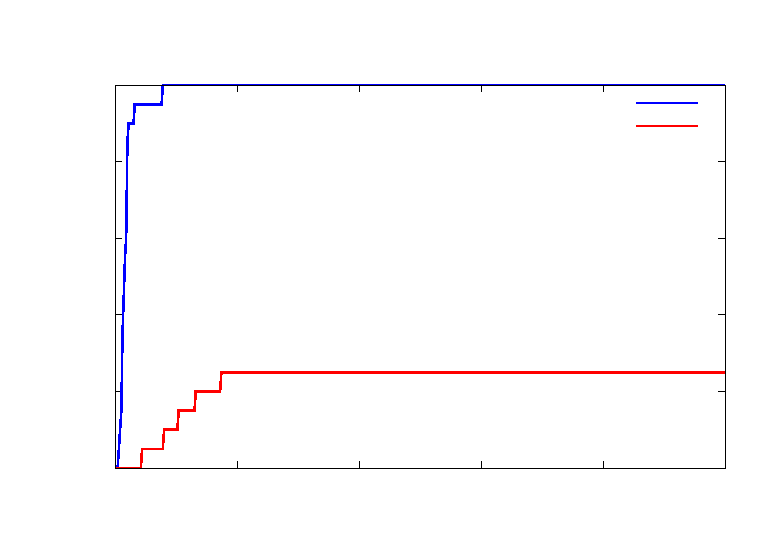
\includegraphics{gnuplot/Ackermann500Cumulative}}%
    \gplfronttext
  \end{picture}%
\endgroup
}
  \end{tabular}
  \caption{Comparison of cumulative probability of success between individuals generated for the two search regimes of case studies.}
  \label{fig:cummulative}
\end{figure}

\subsection{Auxiliary functions - multiplication}
The evaluation of the {\tt Evolve} algorithm was performed with a theory consisting of one datatype for the naturals ($0$ and $s$). We use the constructor style functional scheme (\ref{constructive-style-mul-scheme}) and the destructor style functional scheme (\ref{destructive-style-mul-scheme}) to synthesize the multiplication of natural numbers.

The syntactic equivalence of individuals technique detected that $9.98\%$ of the individuals synthesized were equivalent module $\mathcal{R}$ using functional scheme (\ref{constructive-style-mul-scheme}) and $25.4\%$ using scheme (\ref{destructive-style-mul-scheme}). \cbstart We found two equivalent solutions using scheme (\ref{constructive-style-mul-scheme}) and two solutions using scheme (\ref{destructive-style-mul-scheme}). Figure \ref{fig:error}(a) and \ref{fig:error}(b) shows the best-of-generation individuals of 20 independent runs using schemes (\ref{constructive-style-mul-scheme}) and (\ref{destructive-style-mul-scheme}) respectively. Figure \ref{fig:cummulative}(a) provides a comparison of the cumulative probabilities of success between the schemes (\ref{constructive-style-mul-scheme}) and (\ref{destructive-style-mul-scheme})\cbend. %The theory document in Isabelle/Isar notation is presented in \url{http://goo.gl/eECgLz}.

%We found that the {\tt Evolve} algorithm synthesized the target function in 100\% of the experiments and the solution was synthesized in 2 or less generations.

%Functional schemes can be used to invent more than one function at the time. Functional scheme x was used to synthesize multiplication of natural numbers.

\begin{equation}
  \left(\begin{array}{l}
    constructor\textrm{-}style\textrm{-}mul\textrm{-}scheme\ M\ N \equiv \\
    \quad \quad \begin{array}{c}
      \exists f.\,\, \forall x\, y. \phantom{,}
    \end{array}
    \bigwedge \left\{
    \begin{array}{l}
      f\ 0\ y = y\\
      f\ (s\ x)\ y = M\ x\ y\ 0\ s\ (f\ x)\\
      g\ 0\ y = 0\\
      g\ (s\ x)\ y = N\ x\ y\ 0\ s\ f\ (g\ x)
    \end{array}
    \right.
  \end{array}\right)
  \label{constructive-style-mul-scheme}
\end{equation}

\begin{equation}
  \left(\begin{array}{l}
    destructor\textrm{-}style\textrm{-}mul\textrm{-}scheme\ M\ N \equiv \\
    \exists f.\,\, \forall x\, y.\ \bigwedge \left\{
    \begin{array}{l}
      f\ x\ y  =  M\ x\ y\ 0\ s\ IF\ (=)\ (f\ x)\\
      g\ x\ y  =  N\ x\ y\ 0\ s\ IF\ (=)\ f\ (g\ x)
    \end{array}\right.
  \end{array}\right)
  \label{destructive-style-mul-scheme}
\end{equation}

\subsection{Mutually recursive functions - even/odd}
Mutually recursive functions are naturally expressed using our technique. We use the constructor style functional scheme (\ref{constructive-style-evenodd-scheme}) and the destructor style functional scheme (\ref{destructive-style-evenodd-scheme}) to synthesize the even/odd predicates. We found that the {\tt Evolve} algorithm synthesized the target function in 100\% of the cases using both schemes (\ref{constructive-style-evenodd-scheme}) and (\ref{destructive-style-evenodd-scheme}) in 15 or less generations. The syntactic equivalence of individuals technique detected that 0\% of the individuals synthesized were equivalent module $\mathcal{R}$ using scheme (\ref{constructive-style-evenodd-scheme}) and 2.4\% using scheme (\ref{destructive-style-evenodd-scheme}). \cbstart We only found one solution using scheme (\ref{constructive-style-evenodd-scheme}) and one solution using scheme (\ref{destructive-style-evenodd-scheme}). Since the target funciton was trivially synthesized in the firsts generations, we do not include the best-of-generation individuals graph on Figure \ref{fig:error}. We are also not depicting the cummulative probability of success for the same reason.\cbend

%Figure \ref{fig:error}(e) and \ref{fig:error}(f) shows the best-of-generation individuals of 20 independent runs using schemes (\ref{constructive-style-evenodd-scheme}) and (\ref{destructive-style-evenodd-scheme}) respectively. Figure \ref{fig:cummulative}(c) provides a comparison of the cumulative probabilities of success between the schemes (\ref{constructive-style-evenodd-scheme}) and (\ref{destructive-style-evenodd-scheme}). The theory document in Isabelle/Isar notation is presented in \url{http://goo.gl/ybXr0E}.

\begin{equation}
  \left(\begin{array}{l}
    constructor\textrm{-}style\textrm{-}evenodd\textrm{-}scheme\ M\ N \equiv \\
    \quad \quad \begin{array}{c}
      \exists f.\,\, \forall x\, y. \phantom{,}
    \end{array}
    \bigwedge \left\{
    \begin{array}{l}
      f\ 0 = True\\
      f\ (s\ x)\ = M\ x\ 0\ s\ g\\
      g\ 0 = False\\
      g\ (s\ x)\ = N\ x\ 0\ s\ f
    \end{array}
    \right.
  \end{array}\right)
  \label{constructive-style-evenodd-scheme}
\end{equation}

\begin{equation}
  \left(\begin{array}{l}
    destructor\textrm{-}style\textrm{-}evenodd\textrm{-}scheme\ M\ N \equiv \\
    \exists f.\,\, \forall x\, y.\ \bigwedge \left\{
    \begin{array}{l}
      f\ x  =  M\ x\ 0\ True\ False\ (\lambda x.\ x-1)\ IF\ (=)\ g\\
      g\ x  =  N\ x\ 0\ True\ False\ (\lambda x.\ x-1)\ IF\ (=)\ f
    \end{array}\right.
  \end{array}\right)
  \label{destructive-style-evenodd-scheme}
\end{equation}

\subsection{Total computable functions - Ackermann}
Total computable functions, such as the Ackerman function, are naturally expressed using our technique. We use the constructor style functional scheme (\ref{constructive-style-ackermann-scheme}) and the destructor style functional scheme (\ref{destructive-style-ackermann-scheme}) to synthesize the Ackerman function. We found that the {\tt Evolve} algorithm synthesized the target function in 100\% of the cases using the scheme (\ref{constructive-style-ackermann-scheme}) and 50\% of the cases using the scheme (\ref{destructive-style-ackermann-scheme}). The syntactic equivalence of individuals technique detected that 24.85\% of the individuals synthesized were equivalent module $\mathcal{R}$ using scheme (\ref{constructive-style-ackermann-scheme}) and 6.62\% using scheme (\ref{destructive-style-ackermann-scheme}).

\begin{equation}
  \left(\begin{array}{l}
    constructor\textrm{-}style\textrm{-}ackermann\textrm{-}scheme\ M\ N \equiv \\
    \quad \quad \begin{array}{c}
      \exists f.\,\, \forall x\, y. \phantom{,}
    \end{array}
    \bigwedge \left\{
    \begin{array}{l}
      f\ 0\ y = s\ y\\
      f\ (s\ x)\ 0 = M\ x\ 0\ s\ (f\ x)\\
      f\ (s\ x)\ (s\ y) = N\ x\ y\ 0\ s\ (f\ x)\ (f\ (s\ x))
    \end{array}
    \right.
  \end{array}\right)
  \label{constructive-style-ackermann-scheme}
\end{equation}

\begin{equation}
  \left(\begin{array}{l}
    destructor\textrm{-}style\textrm{-}ackermann\textrm{-}scheme\ M \equiv \\
    \exists f.\,\, \forall x\, y.\ \bigwedge \left\{
    \begin{array}{l}
      f\ x\ y  =  M\ x\ y\ 0\ s\ (\lambda x.\ x-1)\ IF\ (=)\\
      \quad\quad\quad\quad\quad(f\ (x-1))\ (f\ x)
    \end{array}\right.
  \end{array}\right)
  \label{destructive-style-ackermann-scheme}
\end{equation}

\cbstart We found three solutions using scheme (\ref{constructive-style-ackermann-scheme}) and five solutions using scheme (\ref{destructive-style-ackermann-scheme}).
Figure \ref{fig:error}(c) and \ref{fig:error}(d) shows the best-of-generation individuals of 20 independent runs using schemes (\ref{constructive-style-ackermann-scheme}) and (\ref{destructive-style-ackermann-scheme}) respectively. Figure \ref{fig:cummulative}(b) provides a comparison of the cumulative probabilities of success between the schemes (\ref{constructive-style-ackermann-scheme}) and (\ref{destructive-style-ackermann-scheme})\cbend. %The theory document in Isabelle/Isar notation is presented in \url{http://goo.gl/ayO8Cl}.

\subsection{Limitations and further work}
One limitation of our technique is depicted in the following example. Suppose we want to find a $\lambda$-term with the type $\alpha \to \beta$ where $\beta$ is a specialization or an instantiation of $\alpha$. It is easy to see that no such term exists unless we allow the construction of closed terms, instead of pure $\lambda$-terms, with infinitely many type-instantiation functions $\sigma_{\gamma\to\tau} : \mathcal{T}(\mathcal{F},\mathcal{V}) \to \mathcal{T}(\mathcal{F},\mathcal{V})$ where $\sigma_{\gamma\to\tau}$ instantiate type variables from type $\gamma$ to type $\tau$. In this case, the term $(\lambda x.\, \sigma_{\alpha\to\beta}\ x)$ can be used to embody the term sought. Our technique can be easily extended to avoid this limitation, however we left it as interesting future work.

This work has focused more on genetic programming as an algorithm synthesis technique. However, an interesting further work would be to compare our approach with other other competing techniques to synthesize algorithms not based on genetic programming such as deductive synthesis~\cite{manna1980deductive} or inductive synthesis~\cite{kitzelmann2006inductive,kitzelmann2009inductive}, e.g. comparing the techniques w.r.t. the dimensions described in \cite{gulwani2010dimensions}.

%Isabelle/HOL uses code generator facilities to empower the user to turn higher-order logic specifications into corresponding executable programs in different languages such as SML, Haskell or Scala. In this work we used these facilities to evaluate the fitness function on synthesized functions.

%We can perform this transformation on the functional scheme very easily and fully automatically

%Polymorphic. Non-terminating if-splits (cite).

\subsection{Conclusions}
We have defined a specification mechanism based on higher-order formulas to restrict the solution space of synthesized functions in a GP system. Our technique allows to prove termination of synthesized functions using standard facilities in the interactive proof assistant Isabelle. Our approach to genetic programming was successfully applied to the task of evolving different target functions with different recursion schemes. We found that the specification mechanism proposed is suitable for the tasks to represent different recursion schemes, including general recursion.

\section*{Acknowledgments}
This work has been supported by Universidad Polit\'ecnica de San Luis Potos\'i, Universidad Polit\'ecnica de Victoria and Chalmers University of Technology.

\bibliography{myrefs}
%\bibliography{mybibfile}

\end{document}
